\documentclass[PhD]{uclathes}
\pdfpagewidth 8.27in
\pdfpageheight 11.69in

%\includeonly{
%discussion,summary }
%\includeonly{
%abs_ch,abs_en,introduction,facilities,analysis,results,discussion}
%discussion}

%define some new commands used quite often
\newcommand{\pt}{\mbox{$p_T$ }}
\newcommand{\kt}{\mbox{$k_T$ }}
\newcommand{ \ptsq }{ $p_{T}^{2}$ }
\newcommand{ \qsq }{ $Q^{2}$ }
\newcommand{ \gevsq }{\mbox{GeV$^{2}$}}
\newcommand{\ep}{\mbox{$e+p$}}
\newcommand{\eA}{\mbox{$e+$A}}
\newcommand{\eAu}{\mbox{$e+$Au}}
\newcommand{\dA}{\mbox{$d+$Au}}
\newcommand{\pA}{\mbox{$p+$A}}
\newcommand{ \pion }{ $\pi^{0}$ }

%use only in math mode
\newcommand{ \kp }{ k^{\prime} }
\newcommand{ \gammap }{ \gamma^{*}+N\rightarrow h_{1}+h_{2}+X }
\newcommand{ \gammaA }{ \gamma^{*}+A\rightarrow h_{1}+h_{2}+X }
\newcommand{ \phase }{ dz_{h1}dz_{h2}d^{2}p_{h1\perp}d^{2}p_{h2\perp}  }
\newcommand{\pionp}{\pi^{+}}
\newcommand{\pionn}{\pi^{-}}
%\newcommand{ \vtwos}{$v_{2}$}
%\newcommand{ \pts}{$p_T$}
%\newcommand{ \rar }{\rightarrow}
%\newcommand{ \lar }{\leftarrow}
%\newcommand{ \as }{$\alpha_{s}$}
%\newcommand{ \dAu }{$d$+Au}
%\newcommand{ \pp }{$p$+$p$ }
%\newcommand{ \AuAu }{Au+Au}
\newcommand{ \auau }{Au + Au }
\newcommand{\pp}{$p + p$}
%\newcommand{ \CuCu }{Cu+Cu}
%\newcommand{ \cucu }{Cu+Cu }
\newcommand{ \sNN }{ \sqrt{s_{NN}} }
%\newcommand{ \sqrtsNN}{$\sqrt{s_{NN}}$ }
%\newcommand{ \chg }{$h^{\pm}$ }
%\newcommand{ \chgs }{$h^{\pm}$}
%\newcommand{ \ks }{$K_{S}^{0}$}
%\newcommand{ \lam }{$\Lambda$}
%\newcommand{ \lbar }{$\bar{\Lambda}$}
%\newcommand{ \llbar }{$\Lambda + \bar{\Lambda}$}
%\newcommand{ \cas }{$\Xi$}
%\newcommand{ \xxi }{$\Xi^- + \overline{\Xi}^+$}
%\newcommand{ \oom }{$\Omega + \bar{\Omega}$}
%\newcommand{ \omeg }{$\Omega$}
%\newcommand{ \vtwotwo }{{v_2\{2\}}}
%\newcommand{ \vtwofour }{{v_2\{4\}}}
%\newcommand{ \vtwozdc }{v_2\{\mathrm{ZDC-SMD}\}}
%\newcommand{ \vtwoEcc} {v_2/\varepsilon}
%\newcommand{ \density} {1/S\ dN/dy}
%\newcommand{ \fracHydro} {[\frac{v_{2}}{\varepsilon}]/[\frac{v_{2}}{\varepsilon}]_{\mathrm {hydro}}}
%\newcommand{ \sigmacs} {\sigma c_s}
\newcommand{\rmd}{\mathrm{d}}
\newcommand{\bs}{\boldsymbol}
\newcommand{\dedx}{\mathrm{d}E/\mathrm{d}x}

%\def \epart {$\varepsilon_{\mathrm{part}}$ }
%\def \eparts {$\varepsilon_{\mathrm{part}}$}
%\def \eparttwo {$\varepsilon_{\mathrm{part}}\{2\}$ }
%\def \eparttwos {$\varepsilon_{\mathrm{part}}\{2\}$}
%\def \lt {\mbox{$<$} }
%\def \gt {\mbox{$>$} }
%\def \npart {$N_{\mathrm{part}}$}
%\newcommand{\ket}{$m_{T} - m$ }
%\newcommand{\kets}{$m_{T} - m$}
%\def \sims   {$\sim$~}
%\def \GeVc {\mbox{$\mathrm{GeV}/c$}}
%\def \MeVc {\mbox{$\mathrm{MeV}/c$}}
\def\newblock{\hskip .11em plus .33em minus .07em}
\newcommand{\mev}{\mega\electronvolt}
\newcommand{\gev}{\giga\electronvolt}
\newcommand{\fm}{\femto\meter}
\newcommand{\ach}{A_{ch}}

\usepackage{CJK} %use chinese character

%\usepackage{pinyin}
%for tables
\usepackage{longtable}
\usepackage{multirow} %multirows in the table
\usepackage{array} %extends the options for column formats in tables
%\usepackage{caption}
\usepackage{amssymb}
%\usepackage{amsthm}
%\usepackage{revsymb}
%\usepackage{rotate}
\usepackage{epsfig}
\usepackage{epstopdf}
%\usepackage{eepic}
%\usepackage{epic}
\usepackage{graphics}
\usepackage{graphicx}
\usepackage{grffile} %deal with fig name with ".,_ " .etc...
%\usepackage[center]{caption2}
%\usepackage{wrapfig}
%\usepackage{doublespace}
%\usepackage{multicols}
%\usepackage{supertabular}
\usepackage{amsmath}
\usepackage{mathrsfs}
\usepackage{MnSymbol}
%\usepackage{indentfirst}
\usepackage{fancyhdr}
\usepackage{comment}
\usepackage[squaren]{SIunits}
\usepackage{color}
%\definecolor{ColorName}{rgb}{r,g,b}
\usepackage{subfigure}
\usepackage{url} %add url to references
\usepackage[colorlinks=true,linkcolor=blue,citecolor=blue]{hyperref}

%===========================================================================
\pagestyle{fancy} \rhead{} \chead{}
\lhead{
\includegraphics[height=16mm]{plots/title.pdf}} \rfoot{}
%\lhead{\includegraphics[height=16mm]{plots/CCNULogo.pdf}} \rfoot{}
\cfoot{\thepage} \lfoot{}
\begin{document}

\ifx\href\undefined\else\hypersetup{linktocpage=true}\fi

\begin{CJK*}{UTF8}{gbsn}

% preliminary page info
%\graphicspath{{plots/}} %not used too slow
%\makeintropages
\pagenumbering{gobble}
%\thispagestyle{fancy}
%\fancyfoot[C]{}

\mbox{}\vskip 1.2cm
\begin{center}
{\Large\ 博\hskip 0.4cm士\hskip 0.4cm学\hskip 0.4cm位\hskip
0.4cm论\hskip 0.4cm文}
\end{center}
\vspace{0.2in}
\begin{center}
{\LARGE \bfseries 电子-重离子对撞机上双强子关联的 \\ 胶子饱和效应研究}
\end{center}
\vspace{1.1in}

\mbox{}\hskip 1cm{\Large { \bfseries 论文作者: }  郑亮
}

\mbox{}\hskip 1cm{\Large { \bfseries 指导教师: } 蔡勖,J.H. Lee,殷中宝
}

\mbox{}\hskip 1cm{\Large { \bfseries 申请学位: } 理学博士}

\mbox{}\hskip 1cm{\Large { \bfseries 专业名称: } 理论物理}

\mbox{}\hskip 1cm{\Large { \bfseries 研究方向: } 强作用物质(夸克物质与核物质)物理}

\vskip 1.4in

\begin{center}

{\Large 华中师范大学物理科学与技术学院 \\ \vskip 0.5cm
二零一四年九月}

\end{center}
%\end{titlepage}
%\clearpage

%\ched
%\thispagestyle{empty}

%%% Local Variables: 
%%% mode: latex
%%% TeX-master: "PhDthesis"
%%% End: 

\mbox{}\vskip 0.8cm
\begin{center}
{\Large A Dissertation for Doctor of Philosophy in Physics}
\end{center}
\vspace{0.22in}
\begin{center} {\LARGE \textbf{The study of gluon saturation \\ via dihadron correlations at a future electron-ion collider}}
\end{center}
\vspace{0.22in}

\begin{center}
\bfseries{
{\Large  by \\   \vskip 0.22in  \vskip 0.4in }
}
\end{center}




\mbox{}\hskip 0.7cm{\Large { \bfseries Supervisor:  %Xu Cai, J.H. Lee, Zhongbao Yin
} }

\mbox{}\hskip 0.7cm{\Large { \bfseries Specialty:  Theoretical Physics} }

\mbox{}\hskip 0.7cm{\Large { \bfseries Research Area: Strongly Interacting Matter Physics} }

\vskip 1.55in


\begin{center}
{\Large
%College \hskip 0.2cm of \hskip 0.2cm Physical \hskip 0.2cm Science \hskip 0.2cm and \hskip 0.2cm Technology \\
College of Physical Science and Technology \\
Central \hskip 0.2cm China \hskip 0.2cm Normal \hskip 0.2cm University \\ 
\vskip 0.22cm September \hskip 0.2cm 2014 }
\end{center}
%\thispagestyle{empty}

\clearpage


%\pagenumbering{}
\pagenumbering{roman}

%\cleardoublepage\phantomsection
%\addcontentsline{toc}{chapter}{Chinese Abstract}
\pagenumbering{roman}

\chapter*{\LARGE  \bfseries {摘\ \ 要} }


\qquad 研究原子核及其核子的结构和它们之间的相互作用是核物理研究的主要内容。这一类研究揭示了构成我们可见物质世界中的绝大部分质量组分的基本微观性质。
过去半个多世纪的研究工作表明,原子核内的核子是由叫做夸克的基本粒子通过交换胶子的相互作用被束缚在一起而形成的。
为了理解和描述这一类基本相互作用,量子色动力学(quantum chromodynamics,
QCD)在历经半个多世纪的理论与实验工作的交替发展中被逐步建立了起来。通过
QCD框架下的夸克胶子动力学来认识核物质的基本组成被认为是现代核物理研究中的一个重要目标。

QCD中的相互作用基于夸克和胶子所带的色荷。胶子作为相互作用传播子,它本身也带有色荷,这一性质决定了
胶子的自相互作用在核结构的形成中会起到重要的作用。在QCD理论中,与核子发生的碰撞过程通常可以理解为和核子中的
夸克和胶子的一系列基本碰撞过程的非相干叠加,并从中拟合出可普适性地应用于不同碰撞过程的部分子分布函数(parton distribution function,
PDF)以描述夸克和胶子在核子中的密度分布。 过去的实验较好地测定了在核子和轻核中的夸克分布函数,但是对于胶子
的动力学行为还没有能够获得很精确的认识。尤其是对于动量分数比较小(small $x$)的区域,胶子的动力学效应将会
在核子的PDF中占据主导地位。在这一胶子占有数密度比较大、动量分数比较小的动力学区域,胶子的自相互将有可能在核子 的波函数中引起一个被称为胶子饱和的效应。

胶子饱和效应来源于胶子动力学演化中的非线性作用。这一现象在目前的实验中得到了部分的验证,但是由于实验的
精度和模型依赖性的问题,还无法对这一现象的存在以及产生机制得出确定性的结论。未来的电子-重离子对撞机(electron-ion collider, EIC)
将会为解答这一问题提供更多精确的线索。EIC能够提供宽能量范围内的多种核粒子束流。这将为精确 确定胶子行为提供良好的实验条件。

在本文中,我们通过蒙特卡罗模拟的方法,研究了通过在EIC上的双强子关联这一观测量来限制胶子的动力学行为以及找寻
胶子饱和效应的可行性。此外,我们还探讨了一种确定电子重离子对撞过程中的碰撞几何特性的方法。我们的研究表明,通过
EIC上的双强子关联测量我们能够精确地判断胶子饱和效应是否存在,并给出在胶子饱和区的胶子动力学特性。

\vspace{4mm}

\noindent
\textbf{关键词:} 电子-重离子对撞机(EIC), 电子-重离子对撞(\eA ), 量子色动力学 (QCD),胶子饱和, 双强子关联


\chapter*{\LARGE \bfseries {Abstract}}

\normalsize { 

Nuclear physics is very concerned about the emergence of the atom, the nucleus
and the nucleons within it, accounting essentially for the visible mass of our
most immediate universe. Studies over the past half a century have revealed that
the nucleons are consisted of quarks in a bounded state through an interaction
based on the exchange of gluons. The quantum chromodynamics (QCD) is founded to
describe and improve our understanding to this interaction based on the
leapfrogging development in related experimental and theoretical fields. It is
the ultimate goal of nuclear physics to understand the nuclear structure from
the dynamics of quarks and gluons within QCD framework.

The interaction in QCD is attributed to the color charge taken by the quarks
and gluons. While gluons are force carrier, they can take color charge themselves.
Due to this unique feature, gluon contribution is expected to be strong in the
formation of nucleon structure. The inner structure of a nucleon can be explored
by smashing it into smaller pieces. The scattering over a nucleon can be interpreted
as the incoherent superposition of scatterings on the fundamental constituent
quarks and gluons, leading us to a universal parton distribution function (PDF)
describing the densities for quarks and gluons in a nucleon. Although past
experiments were successful in determining the quark behavior in the nucleon and
light nuclei, the gluons that determine the essential features of the strong
interactions, remain largely unexplored. Of great interest is especially the
high parton density (small $x$) regime where gluon self-interaction is expected to
dominate and lead to parton saturation. 

The current theoretical impulses suggest that this saturation effect may come
from the nonlinear evolution for gluons. We have got some tantalizing hints
for the existence of such a feature in the current experimental searches, while
no conclusive evidence is obtained. The proposed electron-ion collider (EIC) with
the possibility to collide multiple nuclear beams in a wide energy range is
believed to be an ideal experimental facility to provide us answers in a very high
precision to the search of saturation physics.

Two-particle azimuthal angle correlations have been reckoned to be one of the
most direct and sensitive probes to access the underlying gluon dynamics on the
future EIC. In this thesis, we will report our Monte Carlo studies targeted to
understand the feasibility of performing this dihadron correlation measurement
on an EIC. Additionally, a possible way to constrain the underlying
electron-nucleus collision geometry has been discussed. This method if achieved
can be very beneficial to precisely study of dihadron correlation measurement.
We have shown that it is very promising to carry out this study at the future
EIC experimental facility.


\vspace{4mm}


\textbf{Keywords:} electron-ion collider(EIC), electron-nucleus collision, QCD, gluon saturation, dihadron correlation


}



\tableofcontents
\listoffigures
\listoftables
\newpage %otherwise list of table page starts as the first page with arabic page number

\allowdisplaybreaks %allow objects in align break in pages

\pagenumbering{arabic}
\chapter{Introduction}
\label{chp:introduction}
You may still remember the times when you were looking into the dark blue sky at
a summer night as a young kid. Your little brain could be stormed by numerous
interesting questions. For example, why are the stars shining in the sky? Why
don't they fall down to the earth? Is there anybody living on the stars? If yes,
do they look the same as us? And so on. Curiosity demands that we ask questions.
As we grow up, it's the same human nature of curiosity that drives us to ask
more deeper questions and come up with reasonable answers to those questions.
Particle physicists are a group of people who are driven by the purest human
curiosity to answer the most ambitious questions with the most organized effort.
The task of particle physics is to understand the question what the world is
made of. Mendeleev's periodic table~\cite{Mende:1869} is one answer to this
question but in a very complicated form. The proliferation and periodic
organization of elements in this table strongly suggests a substructure.
Following the same spirit to explore the unknown world as Columbus who
discovered the new lands, standing on the shoulder of Mendeleev, particle
physicists found their way to the terra incognita rooted deeply in the
fundamental structure of our most immediate world.

Starting from the experimental effort of Rutherford~\cite{Rutherford:1911},
people realized that the element in Mendeleev's table is consisting of a single
type of atom built up of electrons and nuclei in a core like formation. The
atomic nucleus sitting at the core of an atom is composed of more fundamental
particles labeled as protons and neutrons. Later discoveries indicate that these
particles are not alone. They are just two particles in a group called hadrons,
in which all the particles undergo strong interactions. Again, the same argument
repeats that the proliferation of these hadrons is an indication for the
existence of more elementary constituents.

Deep inelastic scattering (DIS) is a process that enables us to directly ``see"
the underlying constituents of a particle in a very clean way. To explain the
overwhelming results from DIS and other experiments, the quark parton model is
proposed to understand the microscopic details about the scattering process. It
is developed in this framework that the scattering on the hadronic objects can
be written as an incoherent sum of cross sections from the scatterings on
individual partons following the hadron's parton distribution function (PDF).
More specifically, the partons are referring to the quarks and gluons. Our
current understanding to the basic structure of all the visible matter can be
interpreted within this model. Gluons carry the strong force and
``glues" quarks together into protons, neutrons and, further, all the hard
cores of the atoms making up the matter in our visible universe. The theoretical
and experimental impulse to describe the properties and dynamics of quarks and
gluons has led to the development of quantum chromodynamics (QCD), which is a
cornerstone to understand the emergence of nucleons and nuclei.


Although past experiments were successful in determining the quark behavior in
the nucleon and light nuclei, the gluons that dictate the essential features
of the strong interactions, remain largely unexplored. Of great interest is
especially, when the gluon density grows to a point where the self-interaction
of gluons have become so important that non-linear QCD effects supersede, a
phenomena named saturation. It is a universal behavior of gluons existing in any
hadronic systems ranging from pions, protons to nuclei. To date, it is still not
yet conclusive that such a saturated regime has been discovered at presently
running high energy experimental facilities. This pursuit will be facilitated by
the advent of a proposed high luminosity, high energy electron-ion collider (EIC).


The present thesis is devoted to the phenomenological studies of the dihadron
correlation measurement to be performed at an EIC. In the remainder of this
thesis, we will walk through the general framework of QCD formulated to
understand the successive experimental results paving us the way to the
understanding of the fundamental constituents for our universe in
Chpt.~\ref{chp:theory}. The conceptual formalism of saturation and its
experimental search is briefed in Chpt.~\ref{chp:saturation}. An
introduction of the EIC project at its realization will be described in
Chpt.~\ref{chp:EIC}. In Chpt.~\ref{chp:MC}, we explain our Monte Carlo
simulation tools used in this study. Based on the current EIC conceptual design,
we will discuss our simulation studies of the dihadron correlation in Chpt.~\ref{chp:dihadron}. In the end, we propose a possible geometry
handle in the electron-nucleus collision and explore its prospective
application in the measurements like dihadron correlation in
Chpt.~\ref{chp:geometry}. A summary is given in Chpt.~\ref{chp:summary}.


\chapter{Theoretical framework}
\label{chp:theory}

\section{Quark parton model and DIS}
\label{sec:basicDIS}
By the time of 1960s, people have discovered a large range of hadrons 
in various experiments. And reactions following certain conservation laws
may convert one type of hadron to another type. Analysis performed on these 
conservation laws and the properties of these hadrons indicates that
there exists some common substructure that forms all the hadronic objects ranging
from pions to protons or neutrons.


Suggested by Gell-Mann and Zweig in 1964, a group of point-like particles named
by quarks can be used to describe this fundamental substructures that build up
the hadron hierarchy. For instance, in the naive picture, a proton is made up of
two ``up" quarks and one ``down" quark. These quarks are supposed to be fermions
with fractional charge following SU(3) symmetry. Due to the color confinement
feature of strong force, there is no isolated fractional electric charge ever
seen in a detector. However, although it is impossible to directly detect these
elementary constituents, one can still obtain the their information with the
structureless lepton probes bombarding hadrons similar to the strategies of
``Rutherford-prime" experiment.

This type of study was firstly performed at the Standford Linear Accelerator
Center (SLAC) experiment with 20 GeV electron beams bouncing off proton
target~\cite{Panofsky:1966gq}. The electron proton scattering process performed
at this experiment can be illustrated by Fig.~\ref{fig:DIS_kinematics} with the
notation of \( e(k)+p(P) \rightarrow e(\kp) + X, \) where $X$ represents any
hadronic final systems allowed by conservation laws. The process is mediated by
a virtual vector boson, with 4-momentum given by $q=k-\kp$.

\begin{figure}
\centering
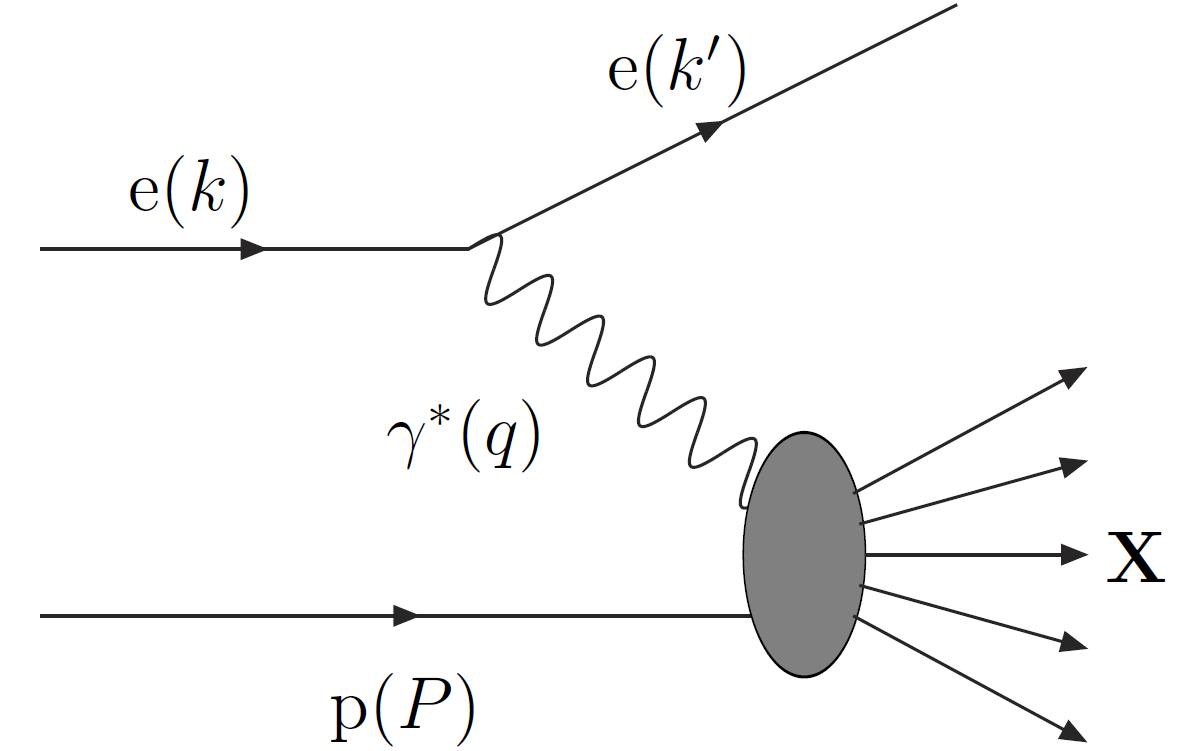
\includegraphics[width=0.5\textwidth]{plots/chpt2/DIS_kinematics.png} 
\caption[DIS scattering diagram] {
Schematic diagram of DIS scattering via virtual photon exchange.}
\label{fig:DIS_kinematics}
\end{figure}

The selection of Lorentz invariant variables describing
Fig.~\ref{fig:DIS_kinematics} is only a matter of convention, but the following
set of the kinematics variables is commonly used:
\begin{enumerate}
\item The squared center-of-mass (CM) energy
\begin{equation}
	s = (k+P)^{2}.
\end{equation}

\item The magnitude of momentum transfer mediated by the virtual boson
\begin{equation}
Q^{2} = -q^{2} = -(k-\kp)^{2},
\end{equation}
at intermediate $Q^{2}$ only photon exchange needs to be considered.

\item Bjorken scaling variable
\begin{equation}
x_{Bj} = \frac{Q^{2}}{2P\cdot q},
\end{equation}
which can be interpreted as momentum fraction of
struck quark taken from the incoming nucleon in the quark parton model.

\item The inelasticity
\begin{equation}
y = \frac{P\cdot q}{ P\cdot k},
\end{equation}
giving fraction of the electron energy transfered to
the hadronic system.

\item The energy current transfered from lepton in the target rest frame
\begin{equation}
\nu = \frac{P\cdot q}{ M_{p} }.
\end{equation}

\item The invariant mass of the final state hadronic system
\begin{equation}
W^{2} = (P+q)^{2}.
\end{equation}

\end{enumerate}

If we define the proton mass by $M_{p}$, the introduced variables are related by
$Q^{2}=(s-M^{2}_{p})x_{Bj}y$, $\nu = ys/(2M_{p})$ and
$W^{2}=M^{2}_{p}+Q^{2}\frac{1-x_{Bj}}{x_{Bj}}$. It can be found in these
equations that only two variables are independent at fixed center-of-mass
energy. If not specified, all the plots in this thesis follow the beam direction
convention: the hadron beam goes to $+z$ and such to positive rapidities are
often referred to as ``forward'' direction, while the electron beam goes to $-z$
and the electron beam going direction is often termed as ``backward'' direction
towards to negative rapidities.



With large momentum transfer \qsq, we are allowed to resolve smaller objects
having transverse momenta less than $Q$ and localized within a transverse
area $\sim 1/Q^{2}$.
The regime of $Q^{2}\gg M^{2}_{p}$ and $W^{2}\gg M^{2}_{p}$ is often referred
to as the DIS regime. Therefore, the proton mass term can be ignored in the relations
for $Q^{2}$ and $W^{2}$ in DIS collisions.

If $Q^{2}$ is much smaller than the mass of $Z^{0}$ boson (neglecting electroweak effects), the DIS process
can be approximately described with the assumption of a one-photon exchange. Then,
the double differential DIS cross section can be expressed as:
\begin{equation}
\frac{d^{2}\sigma}{dx_{Bj}dQ^{2}}=\frac{4\pi\alpha^{2}}{Q^{4}}[y^{2}F_{1}(x_{Bj},Q^{2})+(1-y)\frac{F_{2}(x_{Bj},Q^{2})}{x_{Bj}}].
\end{equation}
In this formula, $\alpha$ represents the fine structure constant. $F_{1}$ and
$F_{2}$ are commonly parameterized frame invariant structure functions for
protons. $F_{1}$ describes the pure magnetic part of the interaction while $F_{2}$
corresponds to the sum over the electromagnetic contribution. A longitudinal structure function can
be defined through $F_{L}(x_{Bj},Q^{2})=F_{2}(x_{Bj},Q^{2})-2x_{Bj}F_{1}(x_{Bj},Q^{2})$,
which reforms the double differential cross section to:
\begin{equation}
\frac{d^{2}\sigma}{dxdQ^{2}}=\frac{2\pi\alpha^{2}}{x_{Bj}Q^{4}}[YF_{2}(x_{Bj},Q^{2})-y^{2}F_{L}(x_{Bj},Q^{2})],
\end{equation}
where $Y=1+(1-y)^{2}$. $F_{2}$ and $F_{L}$ can be practically measured in
inclusive scattering. The \ep\ scattering experiment at SLAC showed that the
structure functions had no dependence on $Q^{2}$, a phenomena called Bjorken scaling 
(for example, see Fig.~\ref{fig:F2_pdg} at $x_{Bj}\sim0.25$).

\begin{figure}
\centering
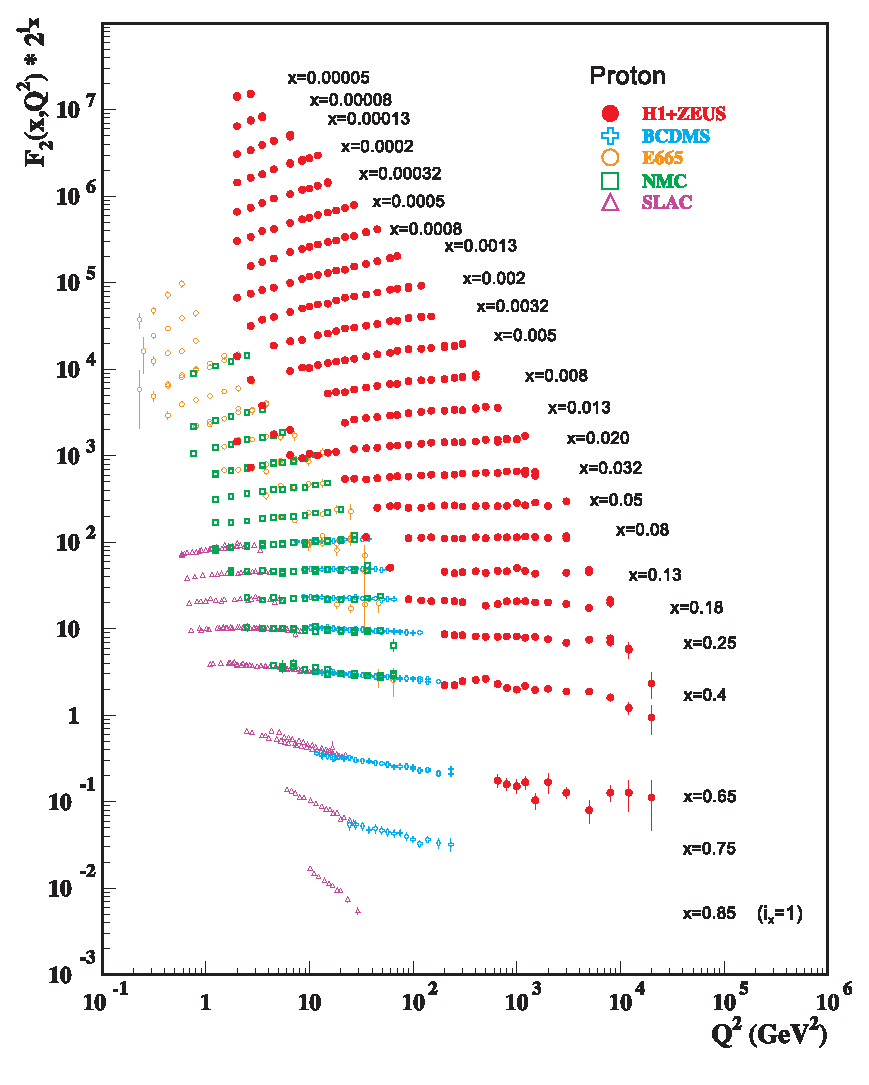
\includegraphics[width=0.85\textwidth]{plots/chpt2/f2collider_logf2.eps}
\caption[proton structure function F2] {
The combined proton structure function $F_{2}$ data from HERA and fixed target experiments at different $x_{Bj}$ (denoted by $x$ in this plot) as a function of $Q^{2}$. The plot is from the PDG tables ~\cite{Beringer:1900zz}.}
\label{fig:F2_pdg}
\end{figure}

The quark parton model was firstly introduced by Feynman to interpret the
scaling behavior observed in the SLAC data. The basic assumption of this model
is to represent the electron proton scattering as an incoherent sum of
scatterings on some individual point-like constituents within the proton called
partons. It is postulated that the partons binded in the proton are effectively
free. To satisfy this requirement, the quark parton model must be defined in the
infinite momentum frame with $P\rightarrow\infty$. In this model, without the
dependence on $Q^{2}$, the structure function $F_{2}$ can be interpreted as
follows
\begin{equation}
F_{2}(x_{Bj})=\sum_{i=q,\bar{q}}e^{2}_{i}x_{Bj}f_{i}(x_{Bj}),
\label{eqn:F2_QPM}
\end{equation}
which sums over partons with charge $e_{i}$. $f_{i}(x_{Bj})$ is the probability
of finding a parton $i$ carrying a fraction $x_{Bj}$ of the proton's momentum.
The $f_{i}(x_{Bj})$ is known as the parton distribution function (PDF). The PDF
is assumed to be universal and can be used for different target particles with
various combinations in a wide range of physics processes. Although the parton
model is shown to be successful in describing a lot experimental data especially
in DIS collisions, a number of paradoxes remain. For instance, there is a clear
breaking to the Bjorken scaling in the $F_{2}$ data at large and small x which
cannot be incorporated in the quark parton model. The study in momentum sum rule
suggests that the momentum carried by quarks and antiquarks do not add up to the
total momentum of protons. This fact implies that there are other important
components in the proton except for quarks and antiquarks. Besides, no
individual quarks ever observed in a free state. These paradoxes shed some light
on the development of QCD as the theory of strong force. We will see how the
puzzles in the simple quark parton model are solved with the elements of QCD
theory derived in the next section.




\section{Quantum chromodynamics} \label{sec:QCD}
QCD is the theory of strong interaction~\cite{Politzer:1974fr}. A gauge
boson, called gluon, is introduced to this framework as the mediator of strong
force. The theory postulates the color degree of freedom with three possible
values, red, green and blue, and correspondingly the anti-colors. The gluons
couple to all particles carrying color charges. While the gluons themselves
carry color charges, it is possible to have gluon self-interactions. The crucial
outcome is that QCD provides the feature of color confinement at large distances
keeping color charges binded in the hadrons and asymptotic freedom allowing to
have essentially free quark interactions at short distances. The strength of
strong interaction is described by the QCD coupling $\alpha_{s}$. This coupling
is predicted to be small in high-energy collisions, which makes it possible to
use perturbation theory in these occasions~\cite{Lipatov:1974qm}.


\subsection{Asymptotic freedom and confinement}
Asymptotic freedom is a feature of QCD that causes forces between partons weaker
as energy increases or distance decreases. This feature arises in a similar way
to the consideration of screening for the electric charge in the quantum
electrodynamics (QED)~\cite{Feynman:1950ir, Gockeler:1997dn}. The vacuum in QED
is assumed to be consisted of virtual electron-positron pair fluctuations in
field theory. In the vicinity of an electric charge, the polarization of these
virtual fluctuations in the vacuum becomes important and partially cancels out
the net charge sitting at the center. The same thing happens in QCD, with the
vacuum being quark-antiquark pairs plus the virtual gluons. Since gluons carry
charge themselves, the vacuum state of gluons in the medium has paramagnetism.
The effect of virtual gluons in the vacuum is to augment the center color charge
instead of screen it, sometimes called antiscreening. So the antiscreening
effect of surrounding virtual gluons at small separations diminishes, the color
interaction becomes feeble under these circumstances (small distance or high
energy). This feature can be mathematically expressed in the running of QCD
coupling $\alpha_{s}$.

\begin{figure}
\centering
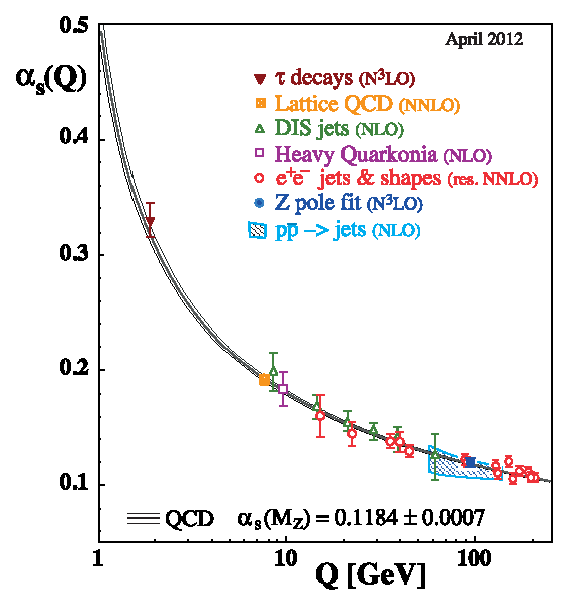
\includegraphics[width=0.5\textwidth]{plots/chpt2/asq.eps}
\caption[Measurement of $\alpha_{s}$] {
Measurements of $\alpha_s$ versus $Q$. The plot is from the PDG tables ~\cite{Beringer:1900zz}.}
\label{fig:alpha_s}
\end{figure}

The derivation of asymptotic freedom in QCD needs to calculate the beta-function
describing $\alpha_{s}$ with the renormalization group equation (RGE). In the
one-loop approximation, the running of QCD coupling $\alpha_{s}(Q^{2})$ is
generally expressed by~\cite{Collins:1987pm}
\begin{equation}
\alpha_{s}(Q^{2})=\frac{4\pi N_{c}}{(11N_{c}-2N_{f})ln(Q^{2}/\Lambda^{2}_{QCD})},
\label{eqn:alphas}
\end{equation}
where $N_{c}$ is the number of color degrees of freedom. $N_{f}$ shows the
number of active quark flavors. $\Lambda_{QCD}$ specifies the energy scale at
which the perturbative coupling becomes infinite. As is shown in
Fig.~\ref{fig:alpha_s}, the coupling $\alpha_{s}(Q^{2})$ becomes essentially
small at large $Q^{2}$.

Formally, Eq.~\ref{eqn:alphas} predicts the divergence of coupling
$\alpha_{s}(Q^{2})$ and the breakdown perturbative QCD theory when $Q^{2}$
approaches $\Lambda^{2}_{QCD}$. But this equation can not be trusted for
$Q\lesssim 1$ GeV, since it is derived from the perturbation theory. Although it
is still debatable about fate of $\alpha_{s}$ for $Q\sim\Lambda_{QCD}$, various
non-perturbative approaches suggest that QCD coupling should be relatively large
(roughly at a value around one). As a consequence, the quarks and gluons should
be confined in the colorless hadrons due to the growth of coupling at low scales
and may not escape as free particles.


\subsection{Factorization}
The microscopic picture of high-energy scattering process involves fluctuated
parton configuration of hadrons in the initial state (see
Fig.~\ref{fig:hadron_config} for an example). We have to deal with the
constantly emitted and absorbed virtual fluctuations in the QCD vacuum. 

\begin{figure}
\centering
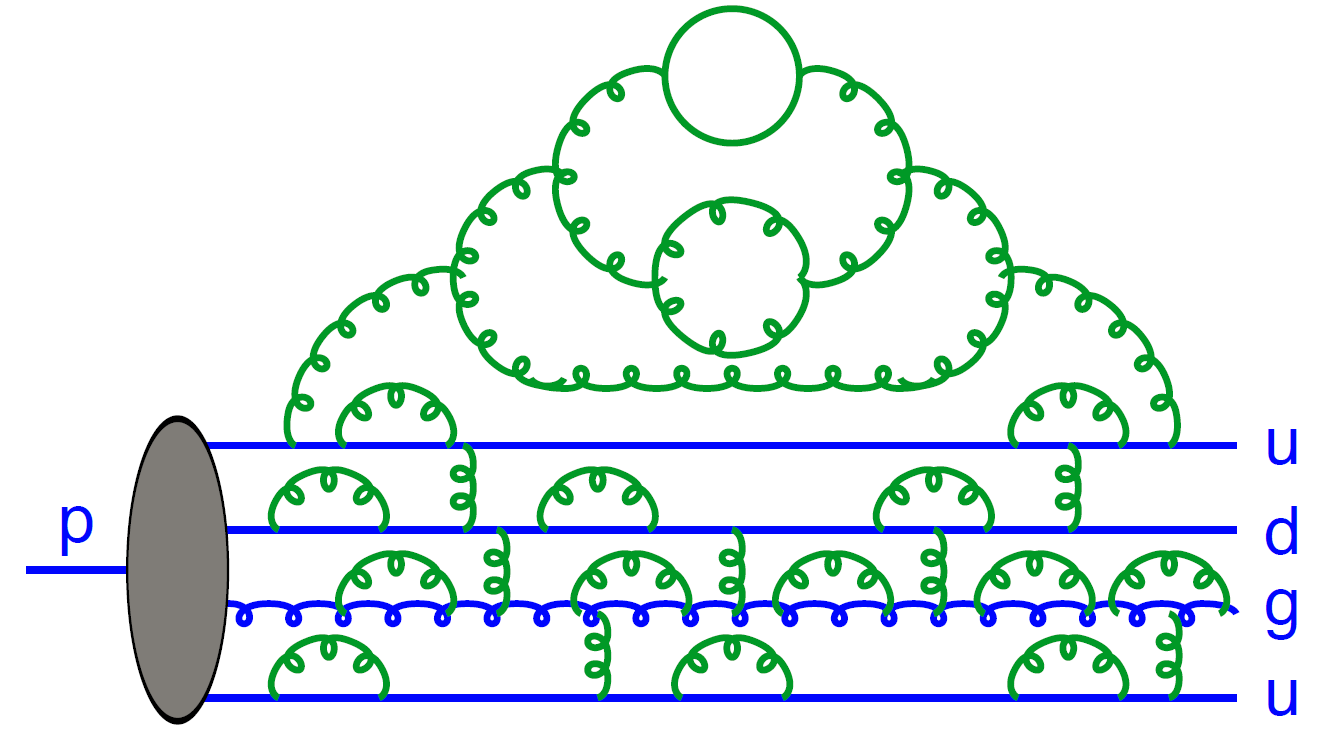
\includegraphics[width=0.5\textwidth]{plots/chpt2/hadron_initial_state.png}
\caption[proton initial state parton configurations] {
Schematic view of proton initial partonic fluctuations. The plot is from Ref.~\cite{Skands:2012ts}. }
\label{fig:hadron_config}
\end{figure}

If we revisit the DIS process illustrated in Fig.~\ref{fig:DIS_kinematics}, we
will find that the virtual fluctuations are confined in the proton with a life
time $\sim 1/\Lambda_{QCD}$. On the other hand, the electromagnetic probe
interacts with the proton at a much shorter time scale $1/Q \ll
1/\Lambda_{QCD}$. During the interaction, the microscopic configuration inside
the proton is almost frozen and can be viewed as a superposition of free,
independent partons (as assumed in Feynman's quark parton model). A snapshot of
the proton inner structure is taken by the virtual photon probe. The scattering
involving a hard probe allowing us to apply the purterbation method like this is
usually referred to as the hard scattering process. Practically, the hard probe
must have a scale $Q^{2}>1 \mathrm{GeV}^{2}$. It is then possible to factorize
the DIS cross section into the product of a process-independent non-perturbative
PDF and a perturbatively calculable hard partonic cross
section~\cite{Sterman:1995fz}.

It is very common to separate the perturbative and non-perturbative parts of the
cross section by applying the collinear factorization scheme, in which the
struck parton is approximately collinear with the proton beam momentum. The DIS
cross section can be expressed in collinear factorization as follows
\begin{equation}
\sigma(ep\rightarrow eX')=\sum_{i} \int^{1}_{0}\frac{dx}{x}f_{i}(x,\mu^{2})\hat{\sigma_{i}}.
\label{eqn:coll_factor}
\end{equation}
$f_{i}$ is the same PDF as explained in Eq.~\ref{eqn:F2_QPM} with $\mu^{2}$
being the factorization scale and $\hat{\sigma_{i}}$ is the hard partonic cross
section. It is convenient to choose the factorization scale to be the exchanged
photon virtuality $\mu=Q$ in DIS collisions. $x$ is the momentum fraction of the
parton involved in the hard interaction. It is equal to $x_{Bj}$ if we focus on
the LO DIS process. For higher oder DIS process, $x$ is larger than $x_{Bj}$ as
shown in the forthcoming discussions. The PDF $f_{i}$ is not priori calculable
and must be constrained by fits to experimental data~\cite{Aaron:2009aa}, while
the partonic cross section $\hat{\sigma_{i}}$ is calculable within the
perturbation theory.


\section{DIS in QCD framework}\label{sec:DISinQCD}
In perturbative QCD (pQCD) framework, for a given physical quantity, the cross
section is calculated by expanding amplitudes in perturbation series of
$\alpha_{s}$. The leading order (LO) DIS diagram is of zeroth order of
$\alpha_{s}$ corresponding to Fig.~\ref{fig:LODIS}, while the next to leading
order (NLO) tree level DIS processes at $\mathcal{O}(\alpha_{s}^{1})$ are shown
in Fig.~\ref{fig:PGF} and Fig.~\ref{fig:QCDC} usually named as Photon-Gluon
Fusion (PGF) process and QCD Compton (QCDC) process, respectively. For the DIS process at LO,
the PGF and QCDC processes are considered as the real corrections, while the
virtual corrections displayed in Fig.~\ref{fig:VirtCorr} also need to be
included. After renormalization, both real and virtual processes will contribute to collinear and soft singularities. It is proven~\cite{Kinoshita:1962ur,Lee:1964is} that for suitable observables, these singularities from real and virtual correction will cancel leaving finite higher order remainders when added together. In the
collinear factorization scheme, these uncanceled collinear singularities with a
scale up to $Q^{2}$ will be absorbed into the scale dependent PDF $f_{i}(x,Q^{2})$. The
scale dependence contributing to the DIS cross section
can be described within the parton evolution scheme. It is expected that the
parton evolution leads to the violation of Bjorken scaling in $F_{2}(x,Q^{2})$.

\begin{figure*}
	\begin{center}
	\subfigure[]{
		\centering
		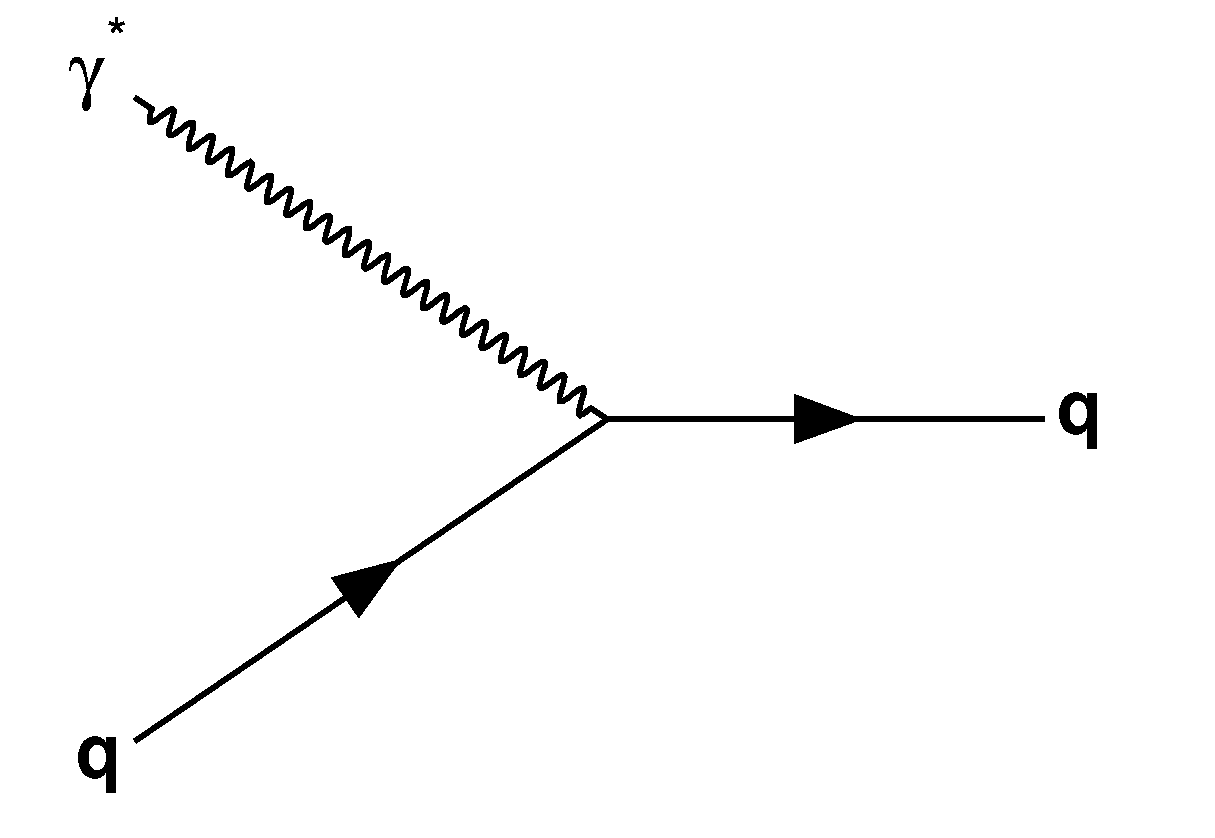
\includegraphics[width=0.25\textwidth]{plots/chpt6/feynman/LODIS.eps}
		\label{fig:LODIS}
	}
	\quad
	\subfigure[]{
		\centering
		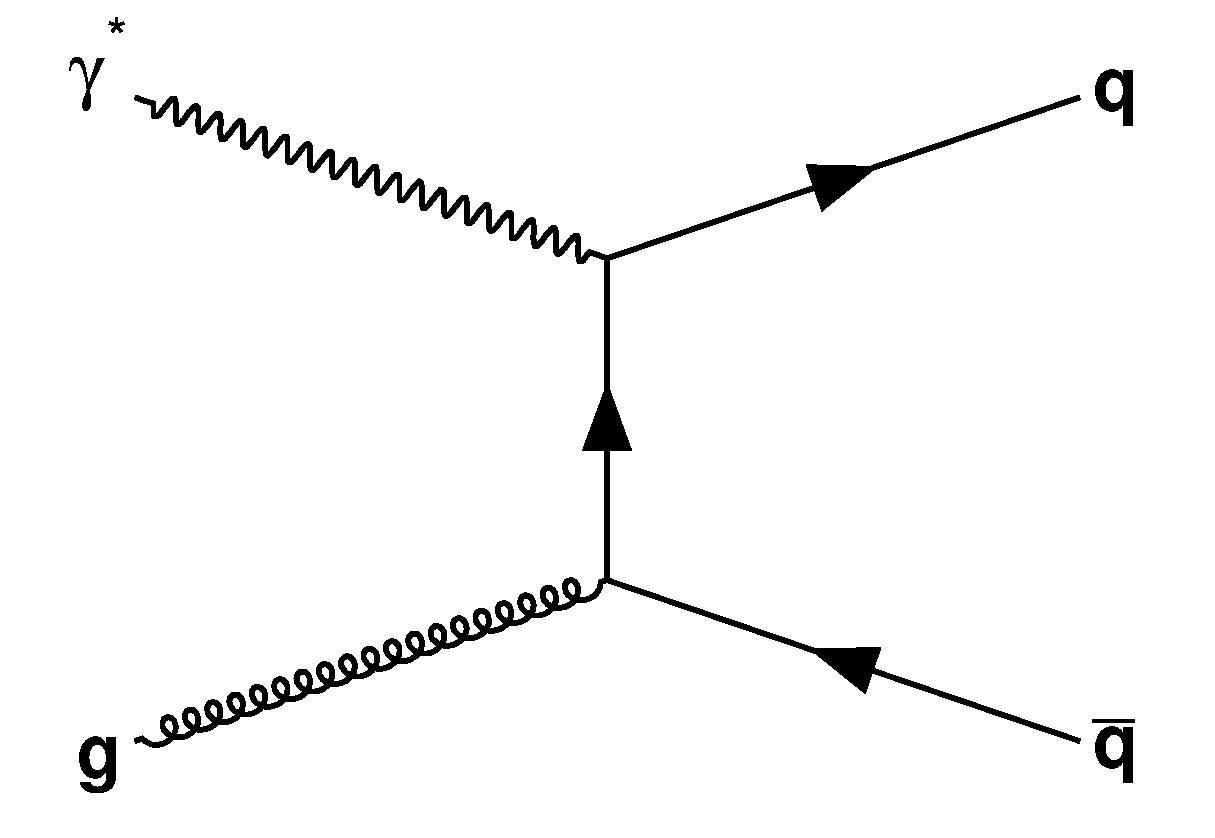
\includegraphics[width=0.25\textwidth]{plots/chpt6/feynman/PGF.eps}
		\label{fig:PGF}
	}
	\quad
	\subfigure[]{
		\centering
		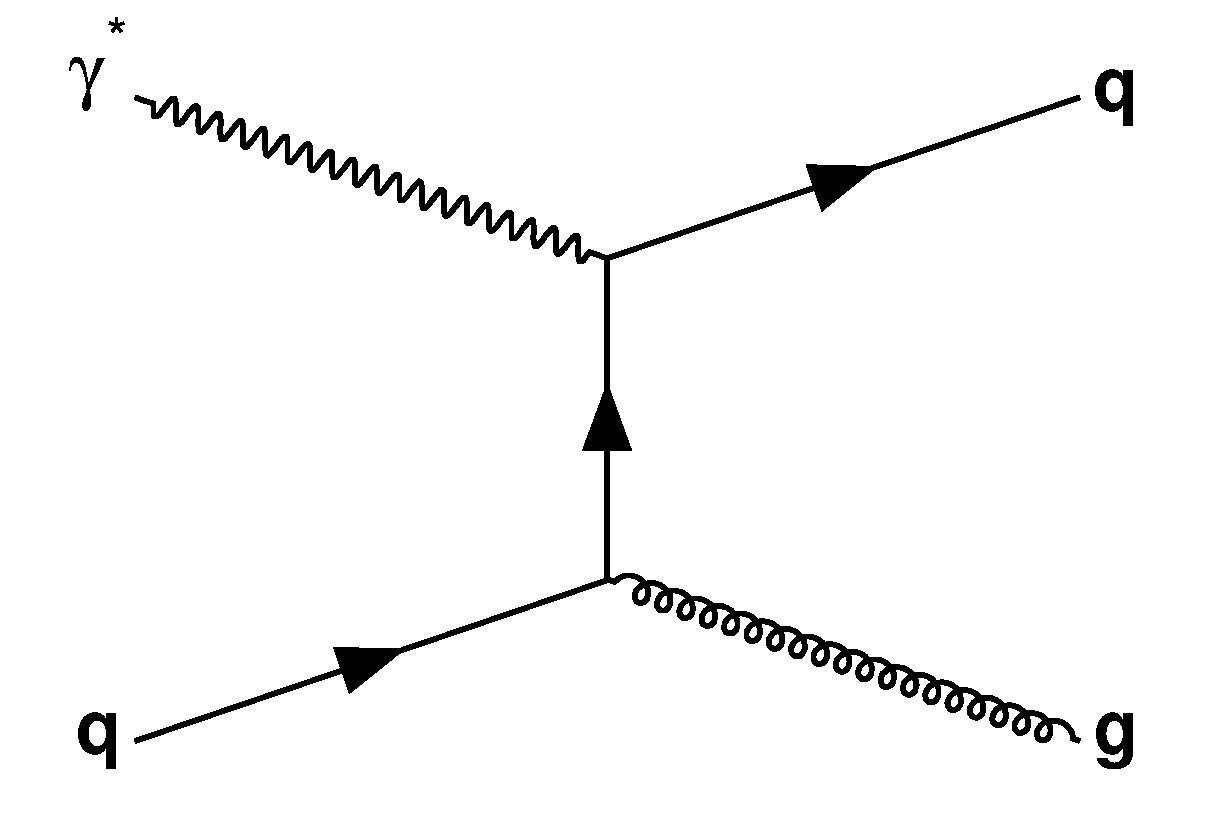
\includegraphics[width=0.25\textwidth]{plots/chpt6/feynman/QCDC.eps}
		\label{fig:QCDC}
	}
	\caption[LO and NLO DIS feynman diagrams]{Feynman diagrams for the hard processes 
	based on point-like photons: (a) $\mathcal{O}(\alpha^{0}_{s}) $ LO DIS, (b) 
	Photon-Gluon Fusion (PGF) and (c) QCD Compton scattering (QCDC).}
	\label{fig:DISgraph}
	\end{center}
\end{figure*}


\begin{figure}
\centering
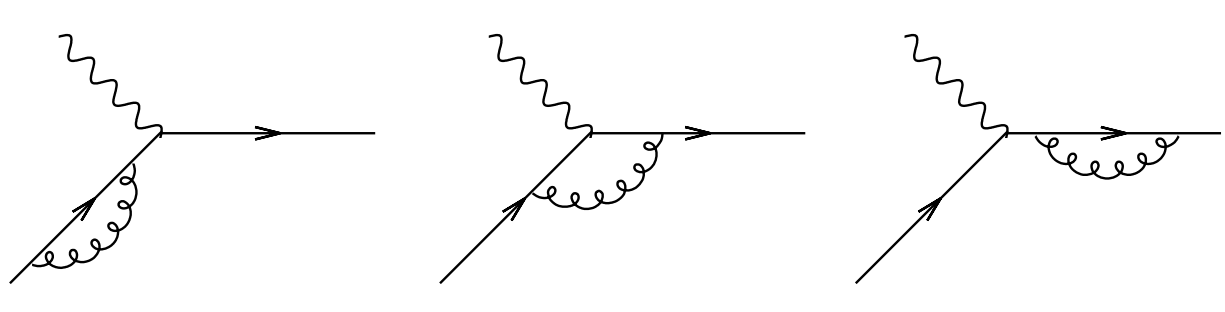
\includegraphics[width=0.8\textwidth]{plots/chpt2/virtual_correction.png}
\caption[virtual corrections] {
Illustration of higher oder virtual corrections to LO DIS. }
\label{fig:VirtCorr}
\end{figure}


\subsection{DGLAP evolution equations}
As is mentioned above, the size and shape of PDF $f_{i}(x,Q^{2})$ is not
calculable in pQCD framework but the scale dependence in $Q^{2}$ for PDF can be
derived from the evolution equations. The $Q^{2}$ evolution of PDF is described
through the Dokshitzer-Gribov-Lipatov-Altarelli-Parisi (DGLAP)
formalism~\cite{Dokshitzer:1977sg,Gribov:1972ri,Altarelli:1977zs}. The essence
of the DGLAP approach is the perturbation treatment of splitting functions. The
splitting functions $P_{ij}(z)$ describe the probability of a
mother parton $i$ splitting into a daughter partons $j$ with momentum fraction
$z$ by emitting a parton $k$ with fraction $1-z$ of the mother parton's
momentum, as demonstrated in Fig.~\ref{fig:split_fun}.

\begin{figure}
\centering
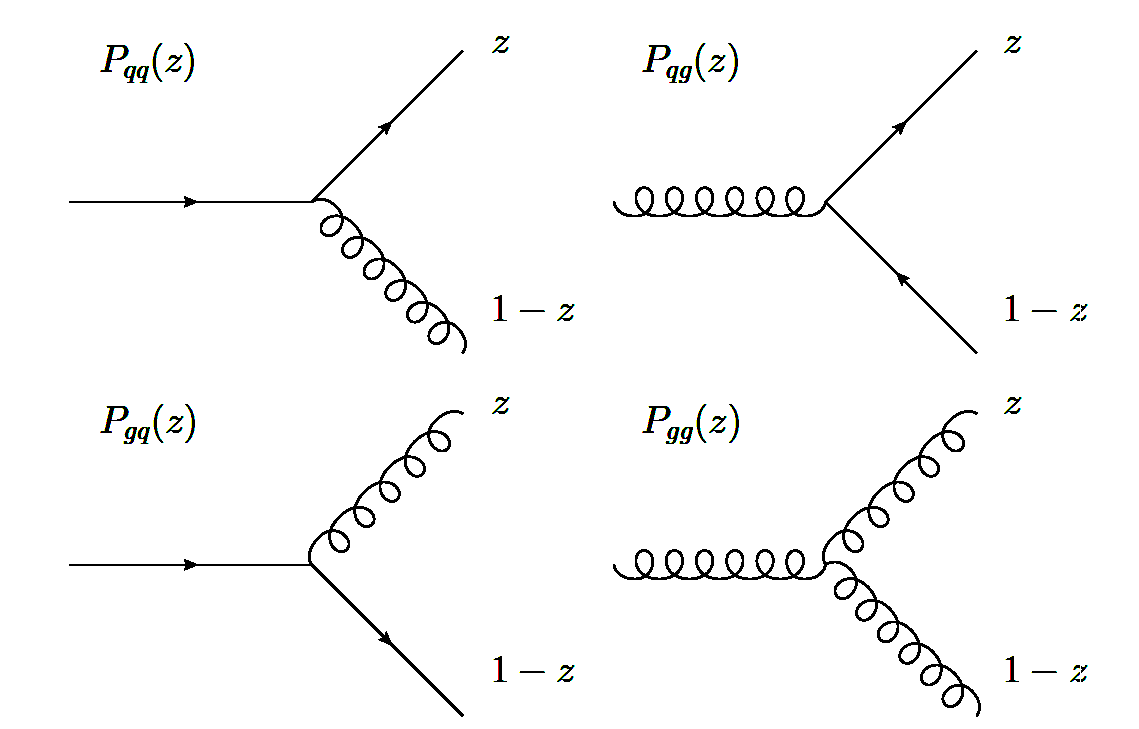
\includegraphics[width=0.5\textwidth]{plots/chpt2/split_fun.png}
\caption[Splitting functions] {
Illustration of diagrams corresponding to the splitting functions. The plot is from Ref.~\cite{Belov:2013oda}. }
\label{fig:split_fun}
\end{figure}

The LO expression for splitting function is given by


\begin{align}
& P_{qq}(z)=\frac{4}{3}[\frac{1+z^{2}}{(1-z)_{+}}+\frac{3}{2}\delta(1-z)], \\
& P_{qg}(z)=\frac{1}{2}[z^{2}+(1-z)^{2}], \\
& P_{gq}(z)=\frac{4}{3}[\frac{1+(1-z)^{2}}{z}], \\
& P_{gg}(z)=6[\frac{1-z}{z}+\frac{z}{(1-z)_{+}}+z(1-z)]+[\frac{33-2N_{f}}{6}\delta(1-z)],
\end{align}


in which $[f(z)]_{+}=f(z)-\delta(1-z)\int^{1}_{0}f(t)dt$.
The DGLAP equations give a rigorous formalism for calculating the changes of PDF
as $Q^{2}$ varies, the PDF shape and size at an initial scale $Q^{2}_{0}$ has to
come either from non-perturbative methods of parameterization in $x$ with
parameters determined by QCD fits to data.

With the DGLAP evolution scheme, the scaling violation effect of $F_{2}$ can be
explained in the QCD framework. As shown in Fig.~\ref{fig:F2_pdg}, the violation
to Bjorken scaling is observed for large $x$ ($x>0.4$) and small $x$ ($x<0.02$)
region. For the large $x$ part, valence quarks dominate the distribution. Since
the struck quark is taking a large fraction of the proton momentum, it is likely
to radiate a gluon as $q\rightarrow qg$. With increasing $Q^{2}$, more gluon
radiations like this will be resolved and the contribution to $F_{2}$ will be
shifted to smaller $x$ value, which is why we see a drop in $F_{2}$ versus
$Q^{2}$. On the other hand, gluons or sea quarks dominate at small $x$. Higher
$Q^{2}$ identifies the process of a gluon splitting into a pair of sea quarks
$g\rightarrow q\bar{q}$, which explains the rise of $F_{2}$ as $Q^{2}$
increases.

\subsection{Evolution at small $x$}
The DGLAP equation in the lowest order resums the leading terms of
$\alpha_{s}\ln(Q^{2})$, while the sub-leading terms involve powers of
$\alpha_{s}\ln(1/x)$. In regions where $x$ is small, the DGLAP approximation is
not valid ($\alpha_{s}\ln(1/x)$ becomes more important than
$\alpha_{s}\ln(Q^{2})$) and a different approach, the so-called
Balitsky-Fadin-Kuraev-Lipatov (BFKL) evolution equation~\cite{Balitsky:1978ic}
has been developed. The BFKL equation is a linear evolution equation and it
governs the evolution of the gluon distribution with respect to $x$ at fixed
$Q^{2}$. The corresponding factorization formula is known as
$k_{T}$-factorization, involving the unintegrated parton distribution function
(uPDF). Then, the \ep\ cross section can be written as
\begin{equation}
\sigma(ep\rightarrow eX')=\sum_{i} \int\frac{dx}{x}dk_{T}^{2}\mathcal{F}_{i}(x,k_{T})\hat{\sigma_{i}}.
\end{equation}
Compared to Eq.~\ref{eqn:coll_factor}, the uPDF can be related to integrated PDF
as \[f_{i}(x,Q^{2})\simeq \int^{Q^{2}}_{0}dk_{T}^{2}\mathcal{F}_{i}(x,k_{T}).\]
At the small $x$, the gluon density grows much faster than the quark density and
is the major component for the proton wave function. Therefore, for the small
$x$ considerations, we shall focus on the gluons alone. The solution of BFKL
equation exhibits a rapid increase of gluon density as $x$ gets smaller.
However, the gluon density cannot grow arbitrarily large, since this would
violate the unitarity limit for forward scattering amplitudes or the Froissart
bound for total cross sections at very high energies. Recent experimental data
at rather small $x$ have provided us some intriguing evidence for the existence
of a novel QCD regime, namely the saturation regime, which cannot be fully
described by linear QCD evolution
approaches~\cite{Stasto:2000er,Armesto:2004ud,Gelis:2010nm}. In the next
chapter, we will have more comprehensive discussions about the physics in
saturation regime.






\chapter{Saturation physics}
\label{chp:saturation}

The idea of saturation physics can be briefly described as follows: when the
gluon density at low $x$ becomes so large that different gluon clouds with fixed
transverse size $\sim 1/Q^{2}$ start to overlap with each other, the QCD
evolution dynamics essentially becomes nonlinear~\cite{Gribov:1984tu,Mueller:1985wy}. 
It is conceivable that gluons which occupy the same area $\sim 1/Q^{2}$ can recombine with a cross section $\sigma_{gg\rightarrow g}\simeq \alpha_{s}/Q^{2}$, thereby taming further
rapid growth of the gluon density (as shown in Fig.~\ref{fig:recombine}). This nonlinear evolution can be encoded by the extension of the BFKL
equation as the Balitsky-Kovchegov (BK) equation~\cite{Balitsky:1995ub}.
\begin{figure}
\centering
\includegraphics[width=0.8\textwidth]{plots/chpt3/recomb.pdf}
\caption[A schematic view of parton recombination process]{
A schematic view of the parton recombination process. This plot is from Ref.~\cite{Accardi:2012qut}.}
\label{fig:recombine}
\end{figure}

This non-linear dynamical effect can be enhanced with a nuclear target, where the
interaction develops over a longitudinal distance of the order of the nuclear size
or larger. 
In this case the nucleons located at the same impact factor
cannot be distinguished from each other. Gluons from different nucleons can
amplify the total transverse gluon density by a factor of $A^{1/3}$ for a
nucleus with mass number $A$. 

\section{Saturation scale}

\begin{figure}
\centering
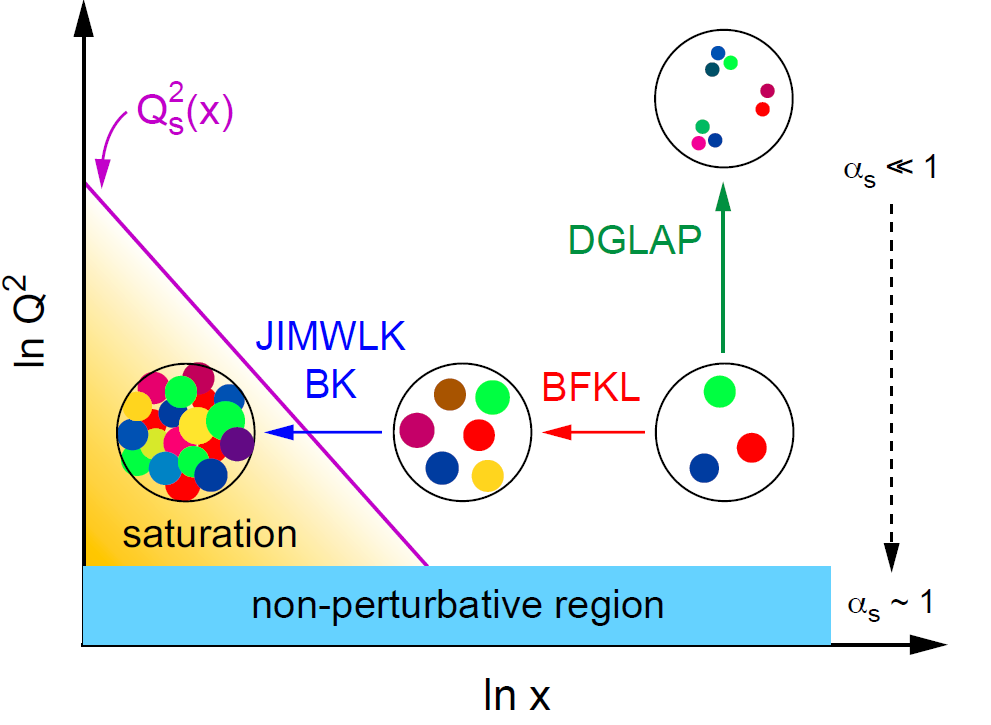
\includegraphics[width=0.65\textwidth]{plots/chpt3/Q2Vx_map.png}
\caption[Evolution approaches in $Q^{2}$ vs $x$ plane]{
Map of high energy QCD in the $Q^{2}$ and $x$ plane. This plot is from Ref.~\cite{Accardi:2012qut}.}
\label{fig:Q2vX_map}
\end{figure}

Typically, a characteristic scale $Q_{s}(x,A)$ can
be introduced to describe the transition to the saturation region. 
\begin{equation}
Q^{2}_{s}(x,A)\simeq A^{1/3} Q^{2}_{0}(\frac{x}{x_{0}})^{-\lambda},
\label{eqn:sat_scale}
\end{equation}
with $\lambda$ known as the saturation exponent. $Q^{2}_{0}$ is the proton
saturation scale at the original value $x_{0}$. These parameters are
non-perturbative and can only be fitted from the data. 
For a large nucleus, the incoming projectile sees the gluons from different nucleons coherently in the longitudinal direction. Note that the transverse gluon occupation number is likely to be enhanced in nuclei by a factor of $A^{1/3}$.
%The generation of the transverse momentum for the scattered projectile on a
%large nucleus can be interpreted as follows: the incoming probe acquires
%transverse momentum kicks from all the nucleons the at the same impact
%parameter. Similar to a random walk process, after $A^{1/3}$ kicks the typical
%transverse momentum generation from a nucleus (or the saturation scale for a
%nucleus target) 
The saturation scale for a nucleus target becomes larger than the proton saturation scale as
$Q_{sA}^{2}\approx A^{1/3}Q^{2}_{sp}$. This enhancement factor $A^{1/3}$ due to
the existence of the nuclear environment is generally named as the nuclear
``oomph" factor.

For $Q^{2}>Q_{s}^{2}$, the target hadron is usually treated as a dilute system,
whereas $Q^{2}<Q_{s}^{2}$ corresponds to the case with a highly dense saturated
hadron with a large parton density. Therefore, as seen in
Fig.~\ref{fig:Q2vX_map}, one can define a boundary with $Q^2=Q_s^2(x)$ in the
$x\textrm{-}Q^2$ plane to describe the transition from the non-linear saturation
regime to the linear dilute regime. The main physical ingredient of the
saturation formalism is to incorporate the unitarity constraint for high-energy
scattering amplitudes through the inclusion of non-linear recombination in the
quantum evolution of hadronic wave functions.


\section{Color glass condensate}\label{sec:CGC}
The partonic form of the matter made with the saturated gluons is known as the
color glass condensate (CGC)~\cite{Iancu:2002xk}. The saturation momentum scale
increases with $1/x$. For sufficiently small $x$, $Q^{2}_{s}>>\Lambda_{QCD}$ and
hence $\alpha_{s}(Q^{2}_{s})<<1$, the CGC is weakly coupled and we should be
able to perform a perturbative calculation. Based on that, our strategy will be
to construct an effective theory, which resums an infinite series of the large
logarithms enhanced by the small $x$. The key ingredient in this scenario is to
describe the small-$x$ gluons as the classical color fields radiated by the fast
partons (valence quarks) with large $x$. Generally, fast partons are seen as the
color source for the classical color fields. The kinematical distinction makes
the foundation for the Mclerran-Venugopalan (MV) model~\cite{McLerran:1993ni}.
With this distinction, we can calculate the non-linear effects exactly within
the classical context.

According to the MV model, the dominant gluon field is given by the solution of
the classical Yang-Mills equations~\cite{Kovchegov:1996ty}, with
which one can construct an unintegrated gluon distribution $\phi(x,k^{2}_{T})$
shown in Fig.~\ref{fig:gluon_TMD}. The majority of the gluons have transverse
momenta $k_{T}\approx Q_{s}$. Unlike the prediction of linear perturbative
theory for the gluon distribution at $k_{T}\sim0$, the growth of gluon distribution
for $k_{T}<Q_{s}$ is largely suppressed or saturated as the name suggests.
\begin{figure}
\centering
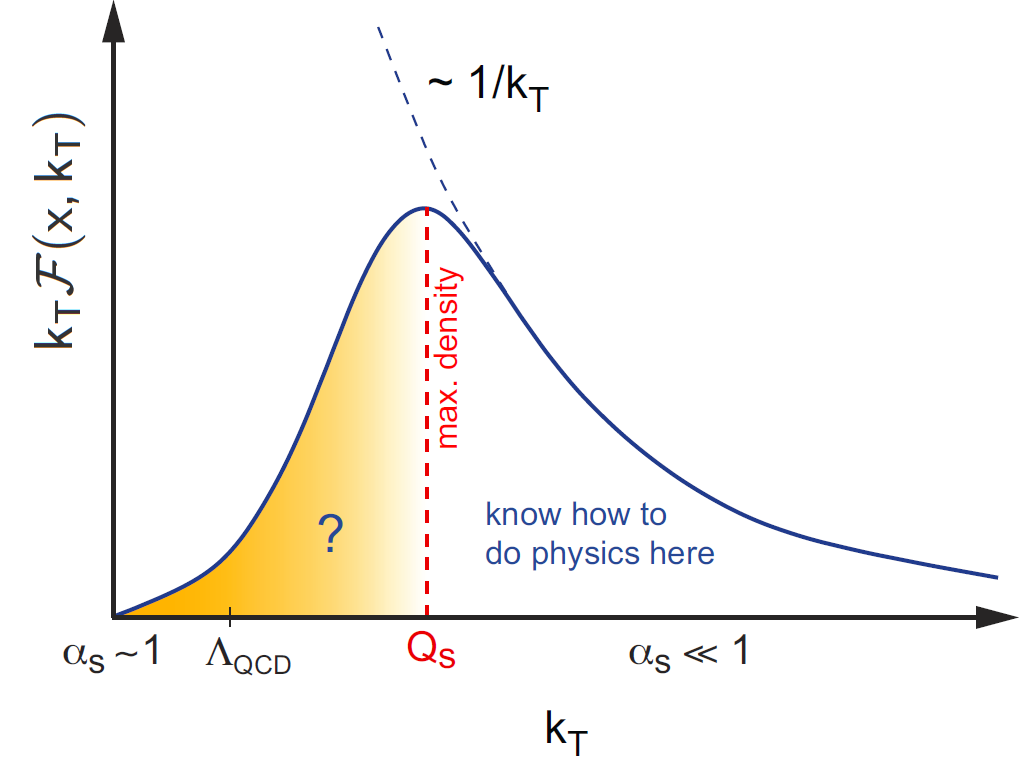
\includegraphics[width=0.65\textwidth]{plots/chpt3/kt_schematic.pdf}
\caption[Unintegrated gluon transverse momentum distribution]{
The unintegrated gluon distribution of a large nucleus from CGC (solid). The dashed curve 
shows the perturbative result with linear evolution. This plot is from Ref.~\cite{Accardi:2012qut}.}
\label{fig:gluon_TMD}
\end{figure}


%
%\subsection{Geometric scaling}
%Geometric scaling is a striking feature of the experimental data observed at
%HERA with $x_{Bj}<0.01$~\cite{Stasto:2000er}, shown by
%Fig.~\ref{fig:geo_scaling}. Generally, one would expect the virtual photon
%proton cross section depends on two kinematics variables $Q^{2}$ and $x_{Bj}$
%independently. However, Measurements at HERA showed that the virtual photon
%proton cross section scales with a single variable $\tau=Q^{2}/Q^{2}_{s}$, in
%which $Q_{s}$ is the saturation scale. Such a scaling behavior has been
%consistently described in the saturation scenario~\cite{GolecBiernat:1998js}. On
%the other hand, the experimentally observed scaling also extends to the kinematics
%region out of the estimated saturation regime. Hence, this scaling feature seems
%to be more general than the saturation and more detailed comparisons with data
%are necessary.
%\begin{figure}
%\centering
%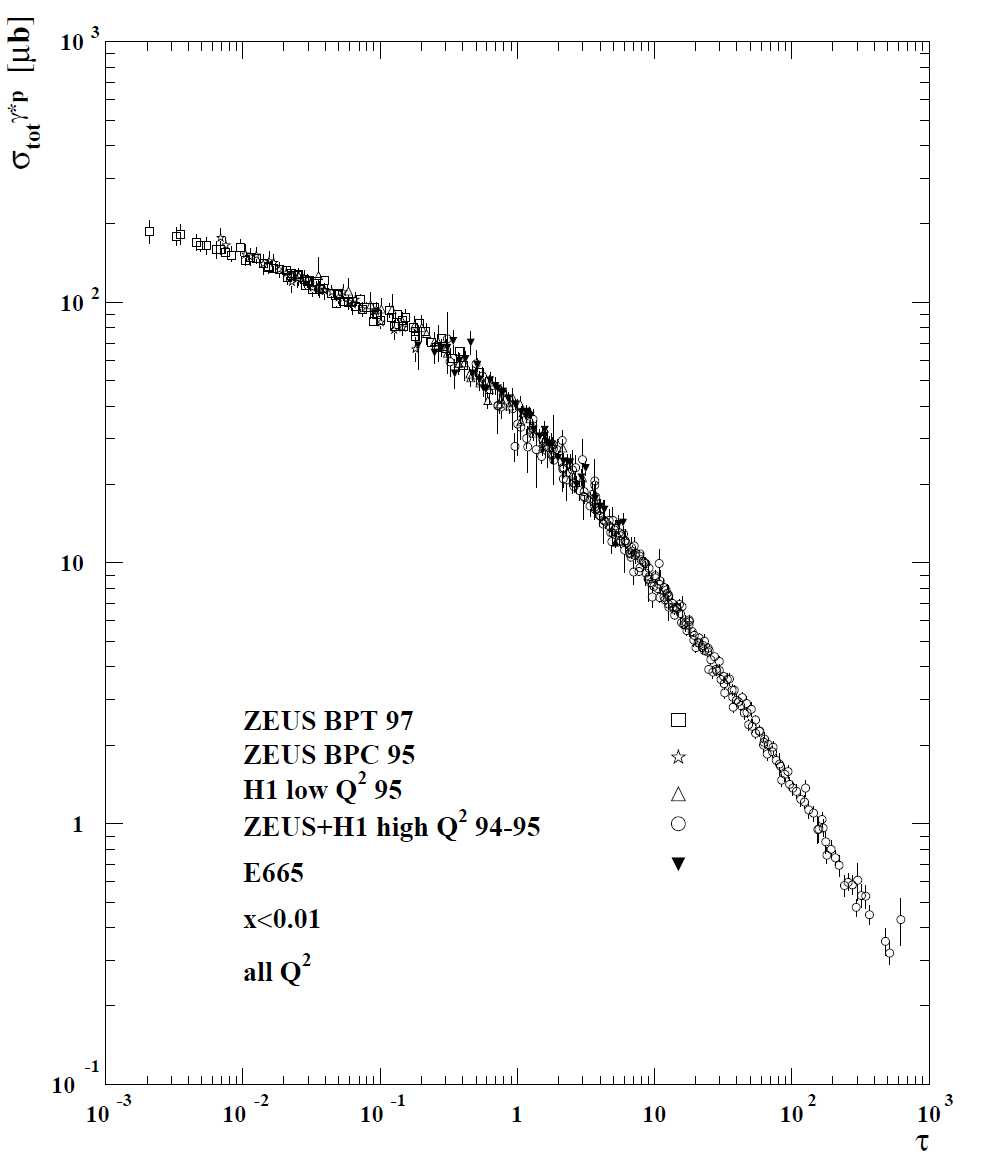
\includegraphics[width=0.7\textwidth]{plots/chpt3/geo_scaling.png}
%\caption[Geometric scaling]{
%Geometric scaling of $\gamma^{*}p$ cross section varying with a single scaling variable
%$\tau=Q^{2}/Q^{2}_{s}$. This plot is from Ref.~\cite{Stasto:2000er}.}
%\label{fig:geo_scaling}
%\end{figure}
%
%\subsection{Nuclear modification factor}
%
%Nuclear modification factor is an observable that has magnetized much of the
%discussion on the saturation physics in $d+$Au collisions at RHIC. In this observable, the nuclear effects can be evaluated in terms of
%the ratio of inclusive particle yields from \dA\ and $p+p$ collisions
%\begin{equation} R_{dAu}=\frac{dN^{dAu\rightarrow
%hX}/dydp_{T}}{N_{coll}dN^{pp\rightarrow hX}/dydp_{T}}. 
%\end{equation} 
%$N_{coll}$ is the number of binary nucleon-nucleon collisions in one \dA\
%collision. If \dA\ collisions were incoherent superpositions of elementary
%nucleon-nucleon collision, the value should be around unity. On the basis of the
%saturation theory, a homogeneous suppression is expected moving from the mid-rapidity
%region to forward rapidities~\cite{Albacete:2014fwa}. It is assumed that in the
%$d+$Au, there's no large final-state effect. Therefore,
%this signature is a clear indication of nuclear effects in the initial state.
%This expectation is observed in the data (see Fig.~\ref{fig:fwd_single_dAu}) and
%a good quantitative description is achieved within the CGC.
%\begin{figure}
%\centering
%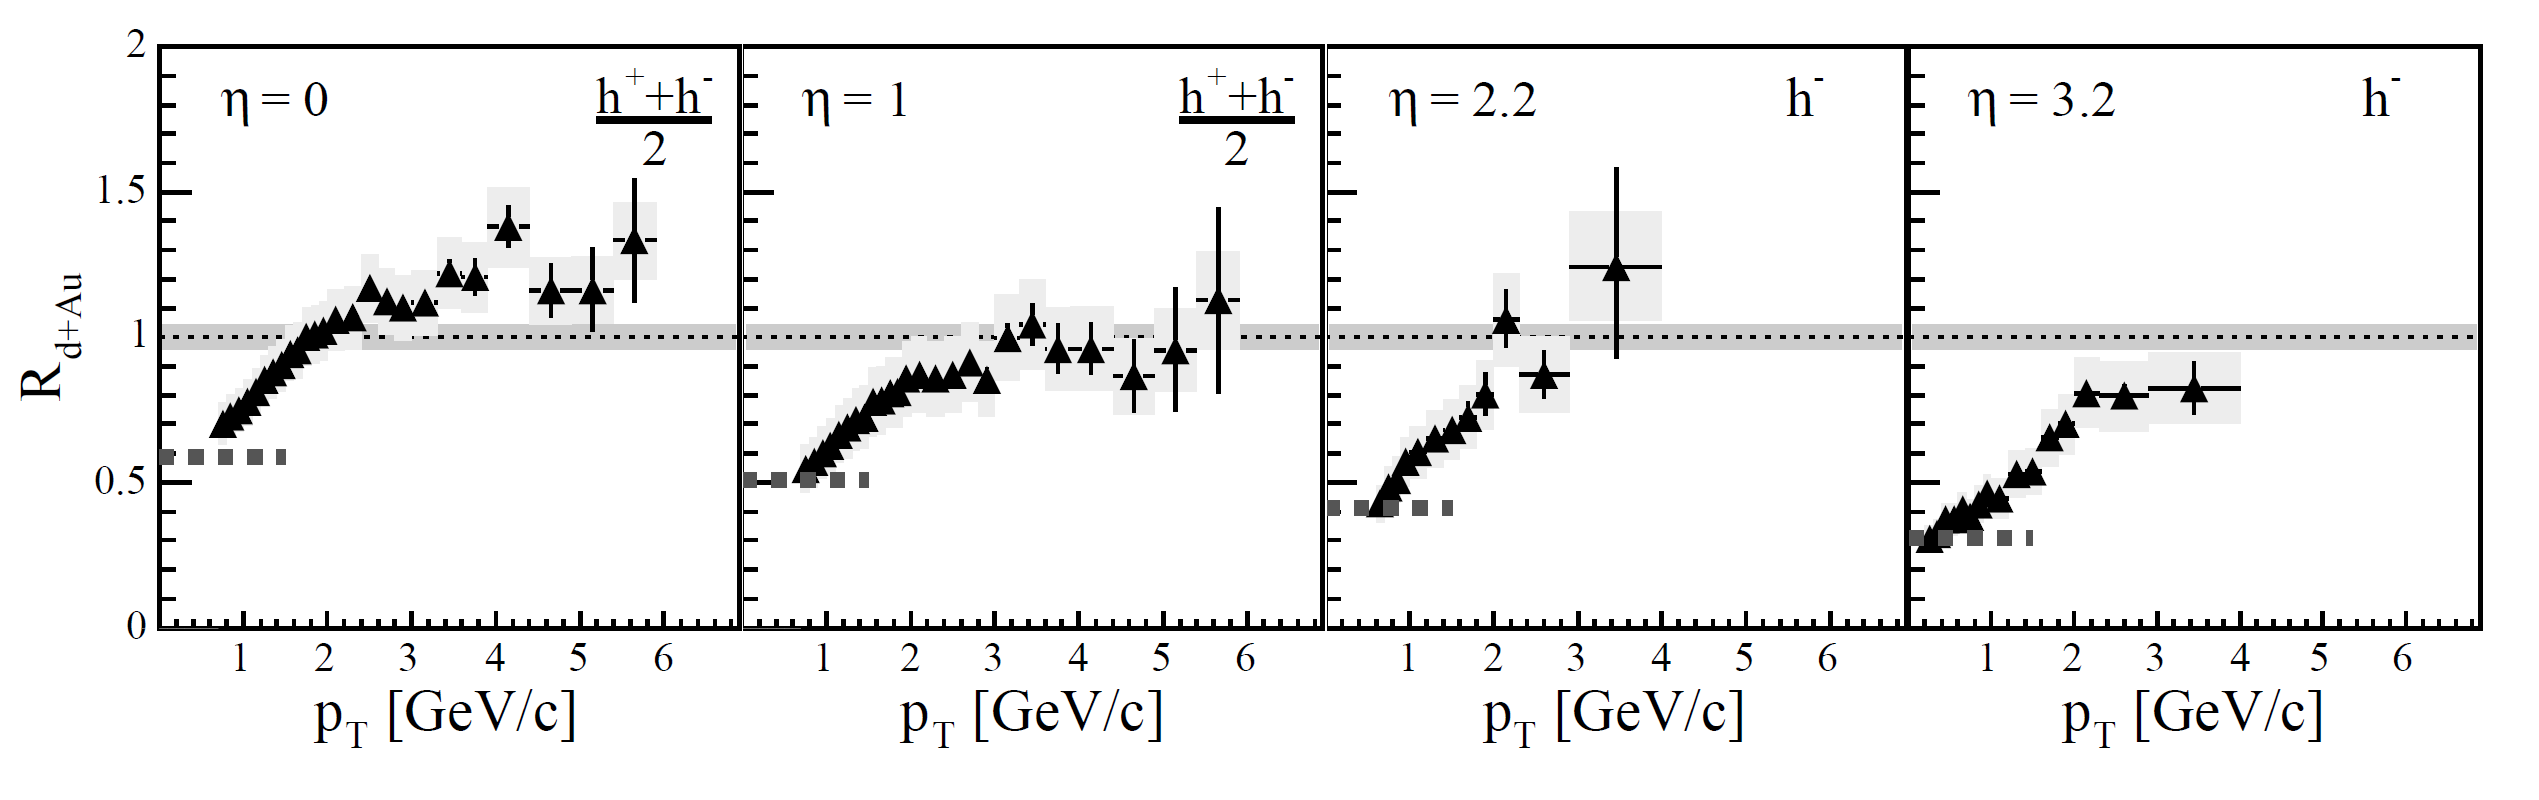
\includegraphics[width=1.0\textwidth]{plots/chpt3/fwd_single_dAu.png}
%\caption[Nuclear modification factors in $d+$Au]{
%Nuclear modification factors from mid-rapidity to forward rapidity region in \dA\ collisions at RHIC. This plot is from Ref.~\cite{Arsene:2004ux}.}
%\label{fig:fwd_single_dAu}
%\end{figure}
%However, other than the CGC approaches, alternative formalisms also reproduce
%the data successfully~\cite{Kopeliovich:2005ym}. It has been argued that large-$x$
%effects such as energy loss neglected in the CGC approach may also be relevant.
%Thus, it is difficult to extract any clean conclusion about the physical origin
%of the forward suppressions. Different physical mechanisms concur and further studies
%are needed.
%


\section{Saturation studies to be performed at an EIC} \label{sec:eic_eA_physics}

It is a challenging task to determine to what extent saturation is present at
currently running high-energy experimental facilities~\cite{Albacete:2010rh}. In
the saturation regime, the interaction is described by the coherent scattering
of the probe from multiple partons collectively correlated in a high density
medium following the CGC picture. To achieve an accurate description of
experimental data, it is essential to have theoretical calculations beyond
the leading order, especially as the higher-order corrections are known to be
sizable. Practically, phenomenological models have been applied to describe a
wide range of experimental data with a few input parameters.

One of the major targets of the \eA\ program at an EIC is to unveil the
collective behavior of densely packed gluons in the saturation regime. As we
argued above, the saturation scale grows with decreasing $x$ and with the
increasing mass number of a nucleus $A$. Collisions with nuclei probe the
saturation region at significantly larger $x$ than would be possible in \ep\
collisions. While at an EIC, it is impossible to directly study the behavior of
saturated gluons in the proton, the $A^{1/3}$ enhancement factor allows us to
perform the saturation studies with large nuclei. We will learn from the
thorough comparison of investigating a multitude of measurements performed on
different ion species. A wide range of measurements with an EIC can distinguish
between predictions from novel theory frameworks like CGC and linear QCD
evolutions established on DGLAP equations.

Compared to the \dA\ program at RHIC, there are several advantages of performing
the saturation studies at an EIC. The predictive power of CGC strongly depends
on the amount of non-perturbative inputs (e.g. initial conditions for small $x$
evolution, impact parameter dependence) needed for the calculations. \eA\
collisions undoubtedly provide the best option to decrease these uncertainties
as much as possible. In addition, with kinematics variables determined event by
event, one can pin down the underlying gluon dynamics more precisely compared to
\dA\ collisions. We will illustrate some key measurements related to the
search of saturation physics at an EIC.

\subsection{Longitudinal structure function}
The total DIS cross section is related to structure functions $F_2$ and $F_L$ by
a linear relation. In the naive quark parton model, transverse momentum of the
partons is assumed to be zero and accordingly we have $F_{L}=0$. The QCD
inspired higher order corrections give rise to partons with non-negligible
transverse momentum and $F_{L}$ becomes nonzero starting from
$\mathcal{O}(\alpha_{s})$ receiving contributions from both quarks and gluons as
shown in Eq.~\ref{eqn:FL}:
\begin{equation}
\frac{F_{L}(x_{Bj},Q^{2})}{x_{Bj}}=\frac{\alpha_{s}}{2\pi}\int^{1}_{x_{Bj}}\frac{d\xi}{\xi}[\sum_{i}e^{2}_{i}\frac{8}{3}(\frac{x}{\xi})q_{i}(\xi,Q^{2})
+{\bar{e}}^{2}4(\frac{x_{Bj}}{\xi})(1-\frac{x_{Bj}}{\xi})g(\xi,Q^{2})], \label{eqn:FL}
\end{equation}
in which $\xi$ shows the momentum fraction of the parton involved in the hard interaction, $q(\xi,Q^{2})$ and
$g(\xi,Q^{2})$ represent the quark and gluon distribution respectively. 
At low $x$, the gluon contribution greatly exceeds the quark contribution. Therefore, measuring $F_{L}$ provides a rather direct
way to study the underlying gluon dynamics with high parton density.

As saturation is mainly driven by the gluon dynamics, we are expected to see
stronger signals in $F_L$. The nuclear effects on the longitudinal structure
function can be quantified as follows:
\begin{equation}
R_{L}(x_{Bj},Q^{2})=\frac{F^{A}_{L}(x_{Bj},Q^{2})}{AF^{p}_{L}(x_{Bj},Q^{2})}.
\end{equation}
In the absence of any nuclear effects, $R_L$ should be unity. 

In Fig.~\ref{fig:F_L}, two calculations for $F_L$ are presented. The blue one is
based on the CGC framework~\cite{Albacete:2009fh}, while the gray band uses the
NLO DGLAP evolution based EPS09 nuclear PDF. For heavy ions $R_L$ shows a
significant suppression due to the existence of the nuclear environment,
while this ratio becomes unity at $A\sim 1$. 
\begin{figure}
\centering
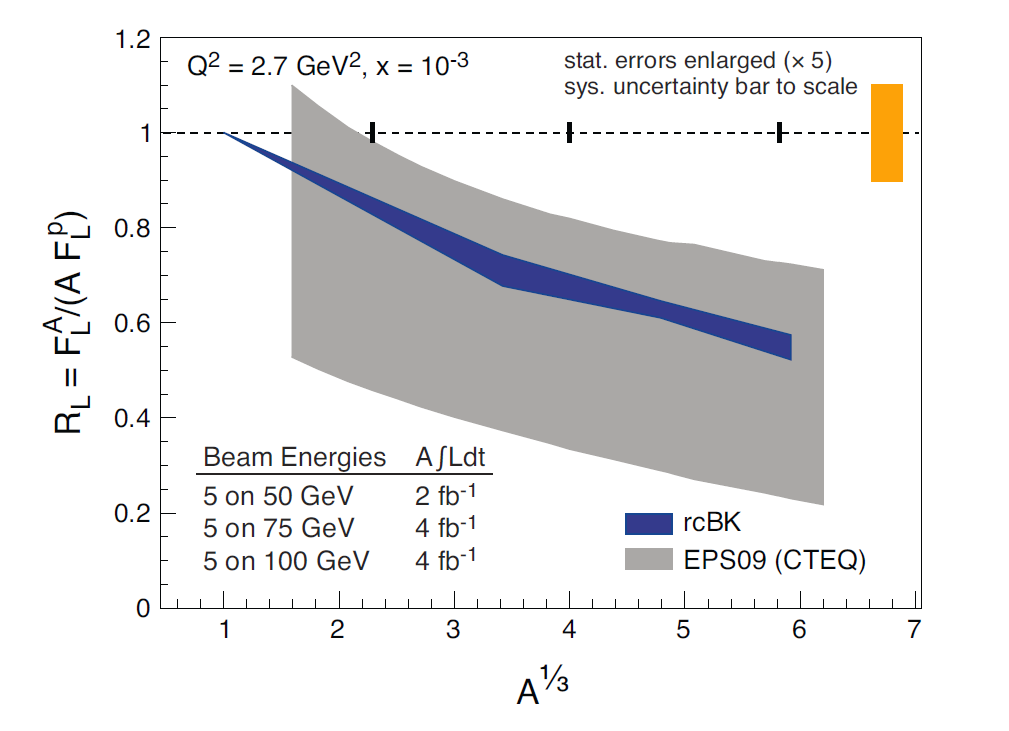
\includegraphics[width=0.7\textwidth]{plots/chpt3/FL_WP.png}
\caption[Longitudinal structure function ratio of different nuclear types over deuteron]{
Monte Carlo data for the ratio of nuclear longitudinal structure function over deuteron. The blue band is from a CGC based calculation while the gray band comes from the EPS09 based DGLAP evolution scheme. This plot is from Ref.~\cite{Accardi:2012qut}.}
\label{fig:F_L}
\end{figure}
Due to the lack of existing nuclear structure function data, the error band on $F_L$ from 
DGLAP approach is very large. The measurements at an EIC will largely constrain the nuclear strucutre
function and significantly reduce the uncertainty for the calculation based on DGLAP approach.
It is expected that with the inclusion of future EIC data, the uncertainty band of DGLAP based
predictions will be small enough to make a discrimination between two approaches.
On the other hand, by the end of the day, it is also possible that the structure function may turn out to be insufficient 
in distinguishing different approaches.


\subsection{Diffractive scattering}
Diffractive interactions happen when the electron probe is coupled to a proton
or nucleus through the exchange of partons without net color. This exchange is
usually named as the ``pomeron", reckoned to be a colorless combination of two or
more gluons.

The HERA data shows that about 15\% of the total DIS cross section is
contributed by diffractive process. One significant feature of the diffractive
process is the existence of a large rapidity gap between the intact
proton/nucleus and the hadronic fragments in mid-rapidity region.

In contrast to the single gluon or quark exchange, two or more gluons exist in
the diffractive exchange. Accordingly, diffractive process is more sensitive to
saturation physics. In \eA\ collisions, the diffractive cross section will be
enhanced compared to \ep\ in saturation model. Thus, the observed amount of
diffractive events is expected to be a smoking gun for parton
saturation~\cite{Kowalski:2008sa}.

Figure.~\ref{fig:diff_eA} shows two calculations for the diffractive process.
The red line is based on the saturation model, while the blue line uses a
leading-twist shadowing (LTS) model. This plot is made versus the squared mass
of the diffractive final state. It is expected to see a significant difference
in the ratio of diffractive events out of total between these two models. The
diffractive process is supposed to be above unity in the saturation model while it
is a bit suppressed in the shadowing model.
\begin{figure}
\centering
\includegraphics[width=0.8\textwidth]{plots/chpt3/diff_Mx2_Q25_x1e-3.pdf}
\caption[Ratio of diffractive cross section out of the total cross section from saturation model and shadowing model]{
The upper plot shows the comparison of the differential diffractive cross section from the saturation model and the leading-twist shadowing model while the lower part shows the ratio of the diffractive cross section divided by the total cross section from these two models. 
\eAu\ results are marked by the dashed lines while solid line is for \ep\ . Saturation model and shadowing model predictions
are plotted in red and blue color respectively. Corresponding $\beta$ value has been labeled against to each $M_{X}^{2}$.
This plot is from Ref.~\cite{Aschenauer:2014a}.}
\label{fig:diff_eA}
\end{figure}

\subsection{Dihadron correlations}  \label{subsec:dihadron_preintro}

Azimuthal dihadron correlations are considered to be a very compelling
measurement to tell whether the partonic system under study has reached the
saturation regime or not~\cite{Kharzeev:2004bw}. The azimuthal angle
$(\Delta\phi)$ distribution of correlated high-\pt hadron pairs uncovers the
underlying jet properties on a statistical basis. The near-side peak
($\Delta\phi=0$) of this $\Delta\phi$ distribution is dominated by the
fragmentation from the leading jet, while the away-side peak ($\Delta\phi=\pi$)
is expected to be dominated by back-to-back jets produced in the hard
$2\rightarrow2$ scattering. At sufficiently high parton densities, when
saturation effects dominate, incoming gluons normally carry a typical transverse
momentum at a scale of $Q_{s}>Q$, which significantly increases the transverse
momentum imbalance of the back-to-back jets. As a result, saturated gluons from
the target tend to smear the back-to-back picture and suppress the away-side
peak in the $\Delta\phi$ distribution.

\begin{figure}
\centering
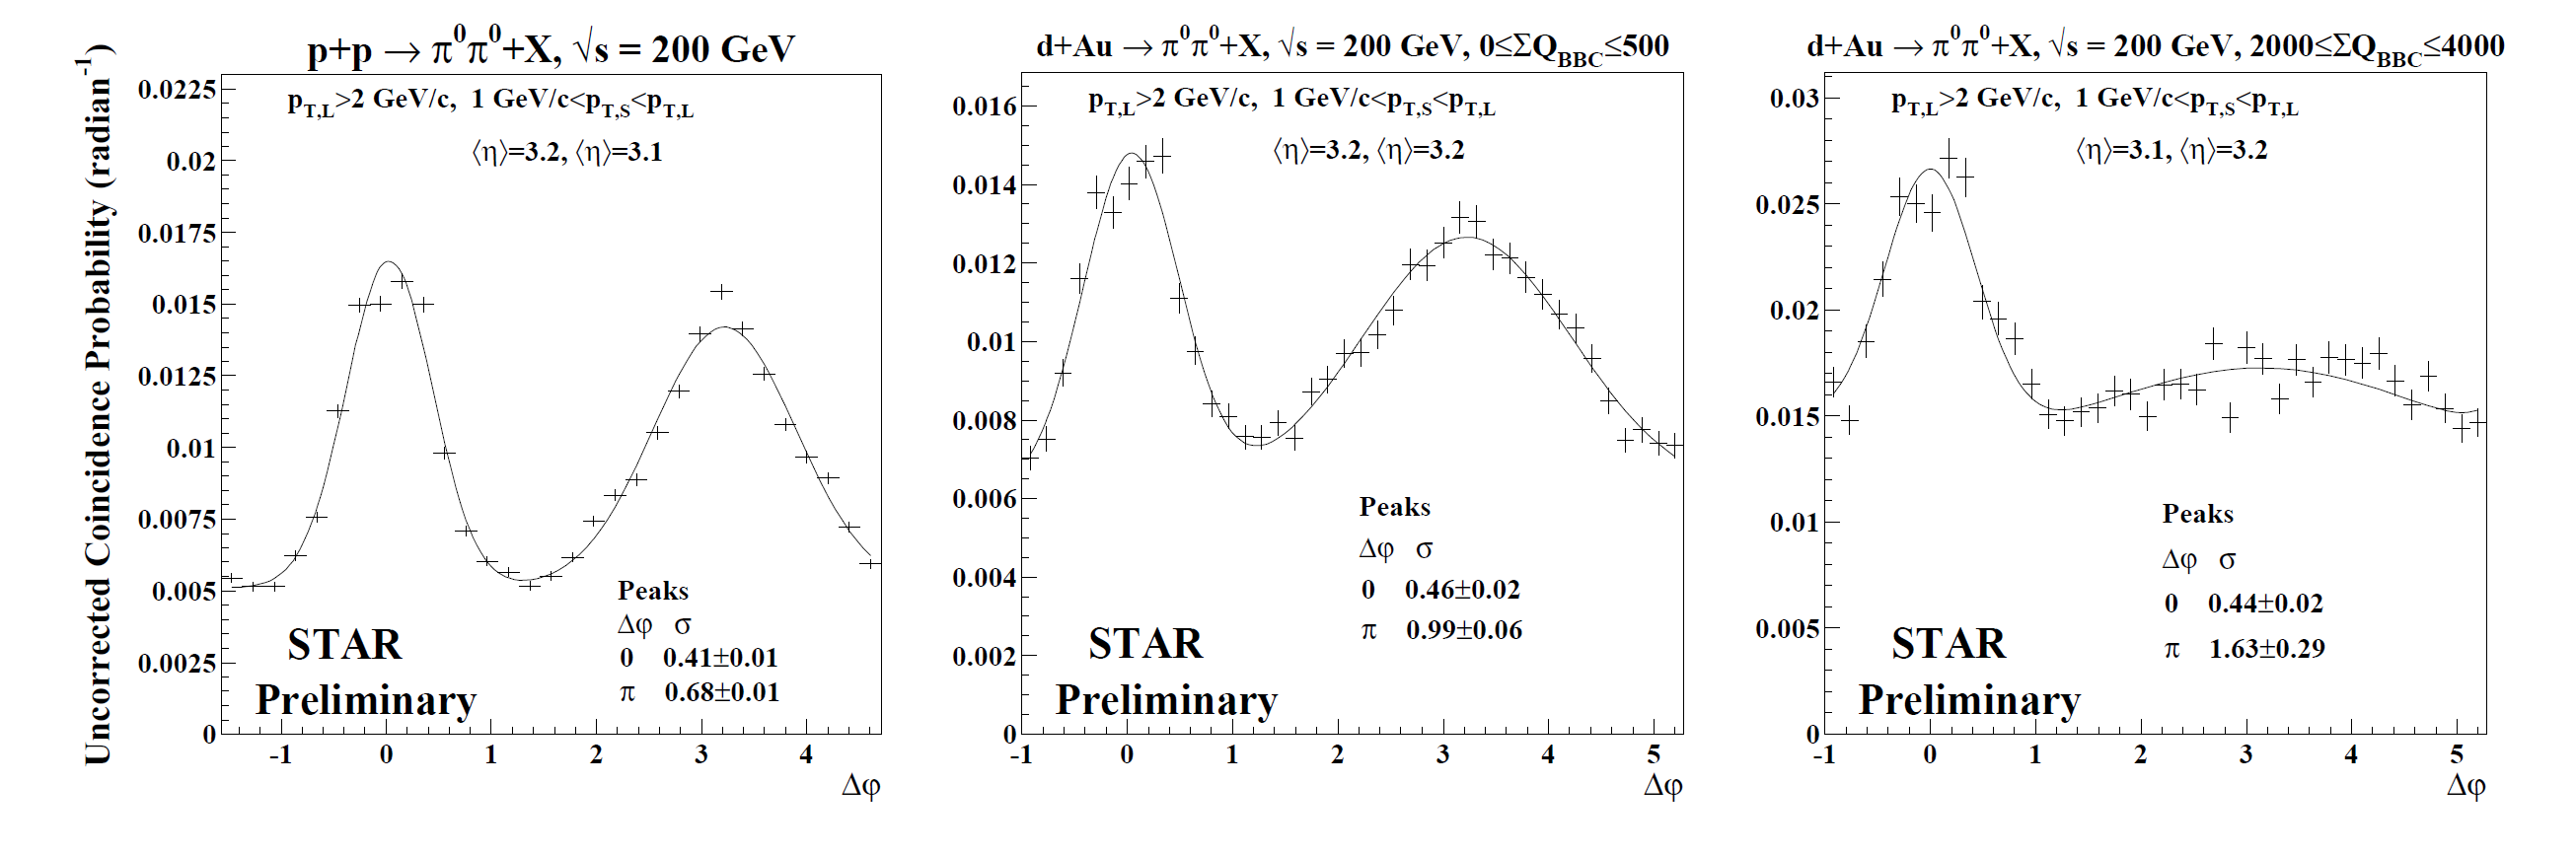
\includegraphics[width=1.0\textwidth]{plots/chpt3/dihadron_pp_dAu_periph_cen.pdf}
\caption[Conditional yield of dihadron correlations in $d+$Au collisions at STAR]{
STAR preliminary results for the two $\pi^{0}$ correlation as a function of the
azimuthal angle difference in $p+p$ and \dA\ ollisions at RHIC. The correlation
function from peripheral and central \dA\ collisions are shown in the middle panel and right
panel respectively.
This plot is from Ref.~\cite{Braidot:2010ig}.}
\label{fig:dihadron_dAu}
\end{figure}

The observed suppressions in dihadron correlation measurements at forward
rapidities performed in \dA\ $\sqrt{s}=200$ GeV collisions at
RHIC~\cite{Adare:2011sc,Braidot:2010ig,Li:2012bn} are perhaps the most
suggestive evidence of the onset of the saturation regime in present data, shown
in Fig.~\ref{fig:dihadron_dAu}. Rather significant suppression of the away-side
correlation is observed, when one compares the data for central \dA\ collisions
to peripheral \dA\ collisions at forward rapidities. The qualitative feature of
this suppression was first predicted by Marquet~\cite{Marquet:2007vb} based on
saturation physics/CGC calculations. The strength of back-to-back correlations
and the depletion of the away-side peak measured in these experiments can be
quantitatively described in the saturation
formalism~\cite{Albacete:2010pg,Stasto:2011ru,Lappi:2012nh}. On the other hand,
a non-CGC framework based on the higher-twist calculation with the nuclear shadowing and the
cold nuclear energy loss correction is also found to be able to reproduce the
suppression phenomenon~\cite{Kang:2011bp}. Generally, the strength of suppression
is expected to be stronger with increasing rapidity, increasing collision centrality
and decreasing transverse momentum of the correlated hadron pairs in \dA\ collisions.


Up to now, it is not possible to extract any definitive conclusion from the
analysis of presently available data. The model dependent kinematics control
introduces a large uncertainty to the data analysis which blurs the
physical interpretation to the phenomenon. Also, the technical difficulty of
higher-order calculations in the CGC also prevents us from achieving a
description of the data precise enough to distinguish different scenarios.
Considering these difficulties, it will be very beneficial to perform the
dihadron correlation study in the \eA\ collisions at an EIC with much better
kinematics control and much less final state contaminations. Besides,
considering it is a single unintegrated gluon distribution structure involved in
\eA\ dihadron correlations instead of a mixture of two types of gluon distribution
involving in \dA\ , the information extracted from the \eA\ dihadron studies will
be complementary to the understanding of phenomenon observed in \dA\ .



At an EIC, we can access dihadron correlations in deep inelastic scattering
(DIS) data from \eA\ and \ep\ collisions, which can provide a clean and
well-controlled signature of saturation physics complementary to the current \dA\
or \pA\ measurements. They also provide the opportunity to study a fundamental
gluon distribution that cannot be accessed today. It has been shown in the
recent theoretical development of small $x$ physics that there are two different
unintegrated gluon distributions (UGDs); namely the Weizs\"{a}cker-Williams (WW)
gluon distribution and the dipole gluon distribution, which are involved in the
calculation of various observables~\cite{Dominguez:2010xd}. Since all other
gluon distributions appearing in various processes can be constructed from these
two UGDs in the large $N_c$ limit of QCD, they can be considered as the
universal and fundamental building blocks for all UGDs. Furthermore, the WW
gluon distribution can be interpreted as the gluon density in the light cone
gauge, while the dipole gluon distribution has no such probabilistic
interpretation. In addition, we want to emphasize that the WW gluon distribution
appears in few physical processes exclusively, and currently there is very
little knowledge about its behavior. Fortunately, the WW gluon distribution is
the only UGD involved in the DIS dijet process~\cite{Dominguez:2011wm}, which
provides us a unique and clean means to measure the WW gluon distribution.




\chapter{Possible realizations of an EIC} 
\label{chp:EIC}

\section{The designing requirement of a future EIC}
The EIC is a multi-purpose collider designed to answer a wide range
of the most compelling science questions concerning to our fundamental understanding of QCD physics. The most intriguing questions
that an EIC will address include:
\begin{itemize}
\item The spin distribution in space and momentum for sea quarks and gluons inside the nucleon.
\item The impact of the nuclear environment cast on the distribution of quarks and gluons and their interactions in nuclei.
\item The collective gluon dynamics in the saturation regime.
\end{itemize}
Two independent designs for the realization of a future EIC have been developed
in the United States. At the Brookhaven National Laboratory (BNL), the eRHIC
design is planning to build a new electron beam inside the RHIC tunnel to
collide with the currently existing polarized proton and nuclear beams at RHIC.
On the other hand, at the Thomas Jefferson National Laboratory (JLab), the MEIC
design utilizes a new electron and ion collider ring complex together with the
recently upgraded 12 GeV CEBAF accelerator at JLab.

The targeted physics programs put some requirements on the EIC machine designs.
To deliver enough physics statistics in a promising time, a high luminosity
$\sim 10^{33} \mathrm{cm}^{-2}\mathrm{s}^{-1}$ is required. Extracting the
structure function and exploring the nuclear time-space evolution needs flexible beam
energy in a wide range. To study the spin distribution, electrons and proton/light
nuclei must be highly polarized. A large variety of nuclear beams are needed to study
the nuclear size dependence. In the semi-inclusive DIS studies, a wide acceptance
detector with good particle identification (PID) is inevitable. For some exclusive
measurements, it is demanding to have the acceptance for protons generated in the
very forward region.

Although the two realizations from BNL and JLab have similar collision parameters,
depending the specific upgrade plan, some differences still exist. For the following
discussions, I will focus on the eRHIC design of the EIC. 


\section{The eRHIC design possibilities}

\subsection{The eRHIC collider parameters}
A cost-effective way of building a full-energy EIC from day one using and an
Energy Recovery LINAC (ERL) with a Fixed-Field Gradient-Accelerator (FFAG)
design is found at BNL as shown in Fig.~\ref{fig:collider_eRHIC}.
\begin{figure}
\centering
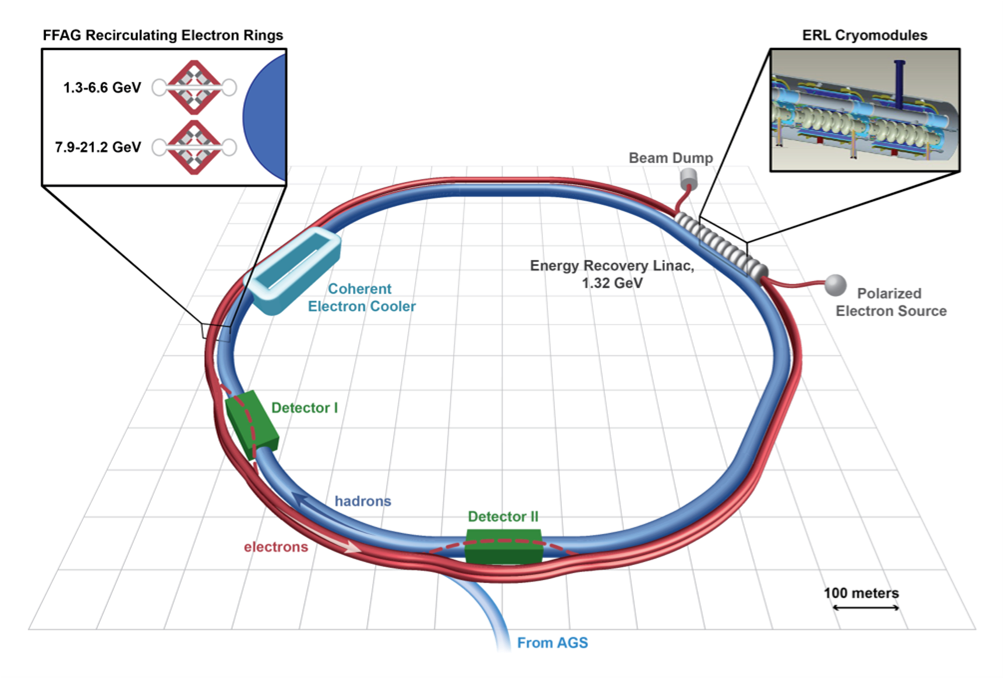
\includegraphics[width=0.9\textwidth]{plots/chpt4/collider_eRHIC.png}
\caption[eRHIC collider design]{
The collider design for eRHIC. The plot is from BNL-CAD eRHIC group.}
\label{fig:collider_eRHIC}
\end{figure}
The current eRHIC machine design allows us to have an electron beam at the
energy ranging from 5 GeV to 21.2 GeV with the beam polarization up to 80\%.
Meanwhile, the existing RHIC facility is capable of providing a proton beam with
70\% polarization at 100-250 GeV. Unpolarized light ions (e.g. dueterium,
silicon) and heavy ions (gold, uranium) are also available to be accelerated to
50-100 GeV/nucleon. There is also the possibility to accelerate the polarized
light ions ($He^{3}$) up to an energy of 167 GeV/nucleon. The full range of
proton/ion beam energies will be accessible from the beginning of operations,
while the electron beam energy will start with 10-15 GeV and later be increased
to 20 GeV. As a result, the available beam energies altogether provide an
accessible center of mass energy range 30-145 GeV.



\subsection{An eRHIC model detector}
To fulfill the requirements on the detector postulated by different physics processes, a generic model detector design has been developed and shown in Fig.~\ref{fig:detector_eRHIC}.
\begin{figure}
\centering
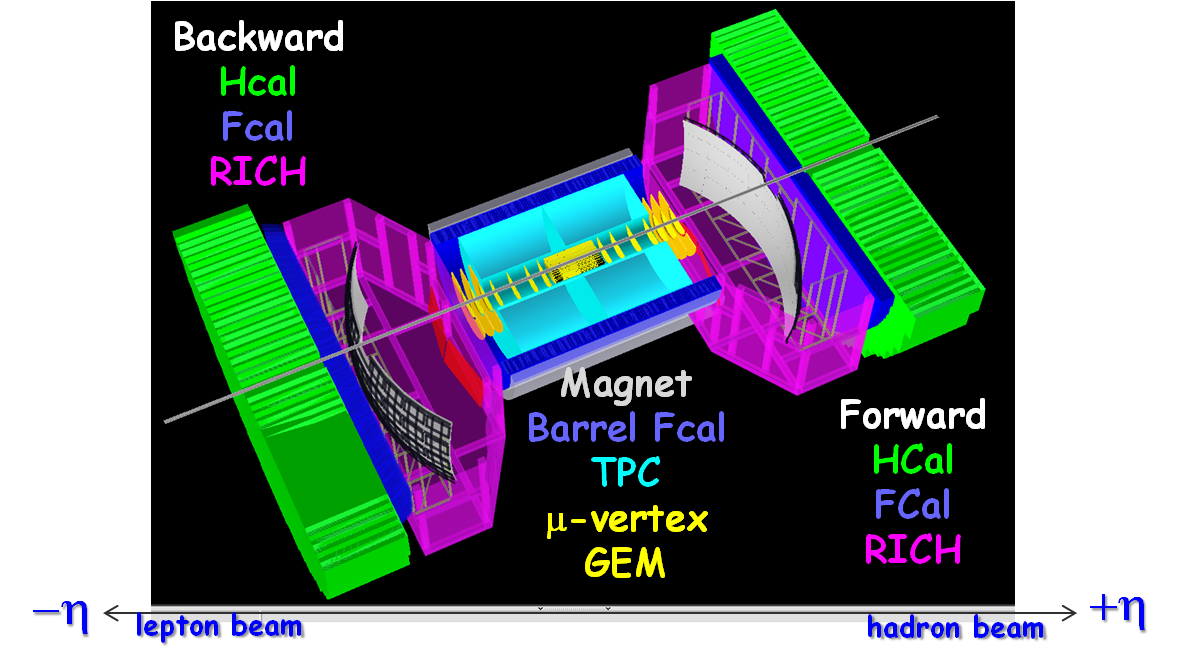
\includegraphics[width=0.9\textwidth]{plots/chpt4/eRHIC_model_detector.png}
\caption[eRHIC detector design]{
Schematics view of the model detector design for eRHIC. The plot is from BNL eRHIC study group.}
\label{fig:detector_eRHIC}
\end{figure}

This eRHIC model detector dedicated to EIC physics is consisted of several major parts.


\begin{itemize}
\item Tracking detectors. The tracking system of the baseline eRHIC detector
will consist of a time projection chamber (TPC), gas electron multiplier (GEM)
and silicon trackers spanning a range $-4<\eta<4$, shown in
Fig.~\ref{fig:tracking_eRHIC}. It is very important to have excellent momentum
resolution over a wide-rapidity range. 
\begin{itemize}
\item Backward/Forward Silicon Tracker: $2<|\eta|<4$, designed with 5-7 MAPS 
(Monolithic Active Sensor Pixels) technology discs.

\item Backward/Forward GEM Tracker: $1.5<|\eta|<3$, designed with 2-3 GEM tracker discs.

\item TPC: $|\eta|<1.5$, deliver hits for pseudorapidity up to $|\eta|\sim2$, but the
range with sufficient number of hits is indicated as above. 

\item Vertex Silicon Tracker: $|\eta|<1$, to be equipped with 4-6 layers of MAPS silicon sensors
similar to the STAR HFT or ALICE ITS upgrade.

\end{itemize}

\end{itemize}


\begin{itemize}
\item Electromagnetic Calorimeter (ECal). The end-cap and barrel regions of
the detector will be equipped with electromagnetic calorimeters covering
$-4<\eta<4$. The different electromagnetic calorimeters have different technologies to account for the different requirements. 


\begin{itemize}
\item Forward ECal: $1<\eta<4$, the requirements for the forward ECal are relatively
moderate as its main function is to detect leptons from the decay of VMs and
photons from dominately $\pi^{0}$ decay. Currently the idea is to have a scintillating fiber tungsten
powder sampling calorimeter. 
\item Barrel ECal: $-1<\eta<1$, this calorimeter needs to provide PID for the scattered lepton at high $Q^{2}$ and leptons from VM-decays, the energy of these leptons will be determined from the tracking detectors. 
The same technology as the forward ECal has been considered for the barrel ECal.
\item Backward ECal: $-4<\eta<-1$, this calorimeter needs to provide PID for the scattered
lepton. It is especially important for the scattered lepton at low $Q^{2}$. At
higher center-of-mass energies photons from $\pi^{0}$ decays, the DVCS and BH
process are in the acceptance of the backward ECal. Since the requirements in
energy and angular resolution are most demanding, it is advised to have a PWO
crystal calorimeter
\end{itemize}
\end{itemize}

\begin{itemize}
\item Hadron Calorimeter (HCal). The resolution requirements for HCal are relatively moderate, therefore standard HCal techniques are totally applicable.  

\begin{itemize}

\item Forward HCal: $1<\eta<4$, this HCal is mainly for jet physics in DIS and diffractive events. It helps define a clean rapidity gap.

\item Backward HCal: $-4<\eta<-1$, this HCal is designed for the jet physics and will be useful to identify scattered lepton at low $Q^{2}$
when ECal is not enough to separate leptons from hadrons. 

\end{itemize}
\end{itemize}

\begin{figure}
\centering
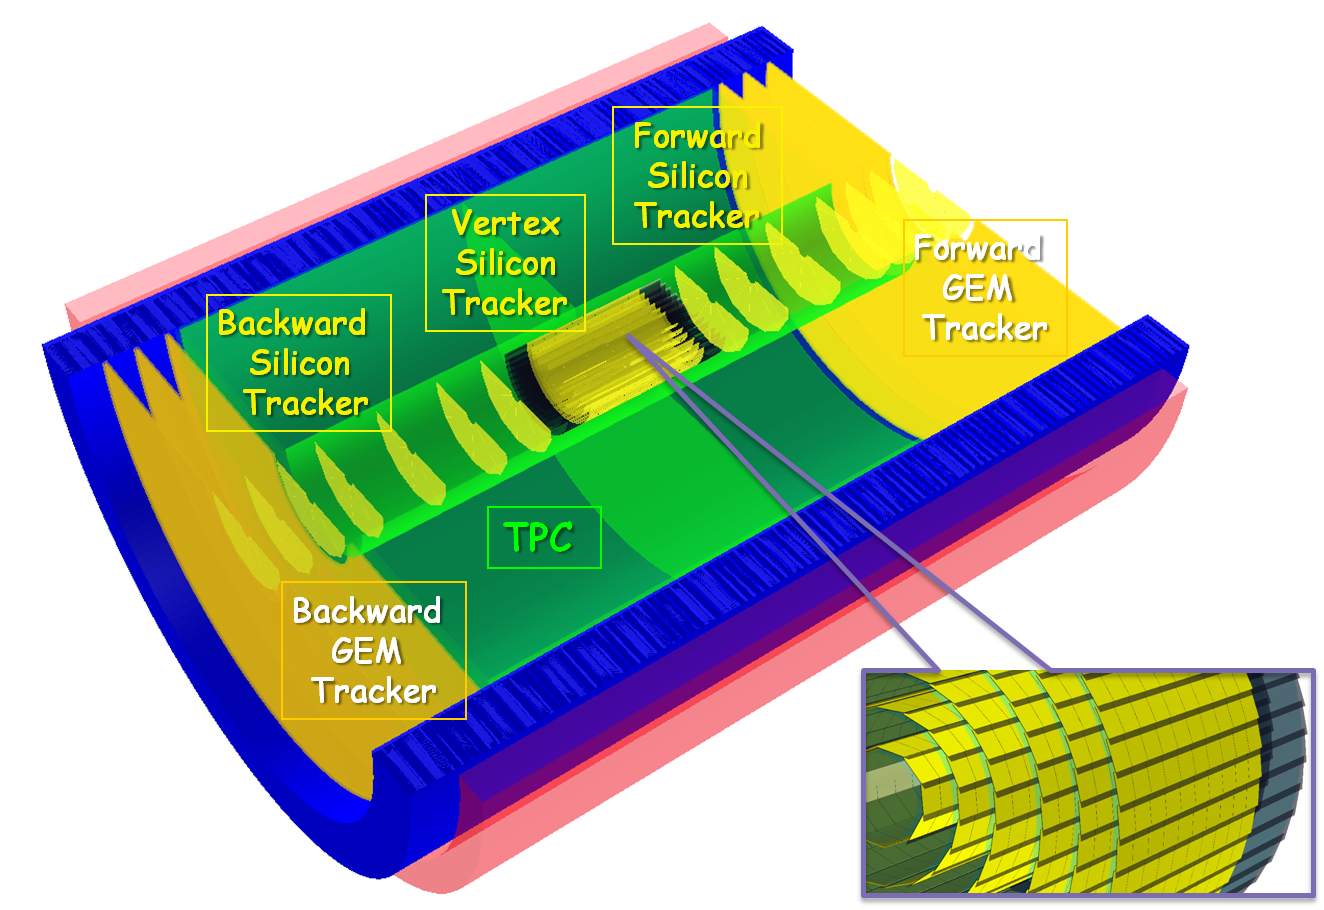
\includegraphics[width=0.9\textwidth]{plots/chpt4/eRHIC_model_tracking.png}
\caption[Tracking system of the eRHIC model detector design]{
Schematic view of the tracking system used in the model detector design for eRHIC. The plot is from BNL eRHIC study group.}
\label{fig:tracking_eRHIC}
\end{figure}


Particle identification for different purpose relies on different combinational
method. $\pi, K, p$ separation can be achieved in central rapidity region
$\eta<1$ with DIRC or proximity focusing Aerogel-RICH plus the $dE/dx$ from TPC
energy loss. The separation in $1<|\eta|<3$ is obtained in RICH, where a very
good meomentum resolution from the tracking is needed.

Lepton identification mainly relies on the $E/p$ in the region $-3<\eta<3$. For
$1<|\eta|<3$, additional HCal response and $\gamma$ suppression via tracking can
be applied to find electrons. In $|\eta|>3$, combinational ECal and HCal
responses and $\gamma$ suppression via tracking will provide a clean access to
the scattered lepton.


\subsection{eSTAR and ePHENIX}
Other than the model detector design which is dedicated to the DIS physics, it
is also possible to evolve the current STAR and PHENIX experimental facility to
eSTAR and ePHENIX~\cite{Adare:2014aaa} in the future with some upgrades. 


\begin{figure}
\centering
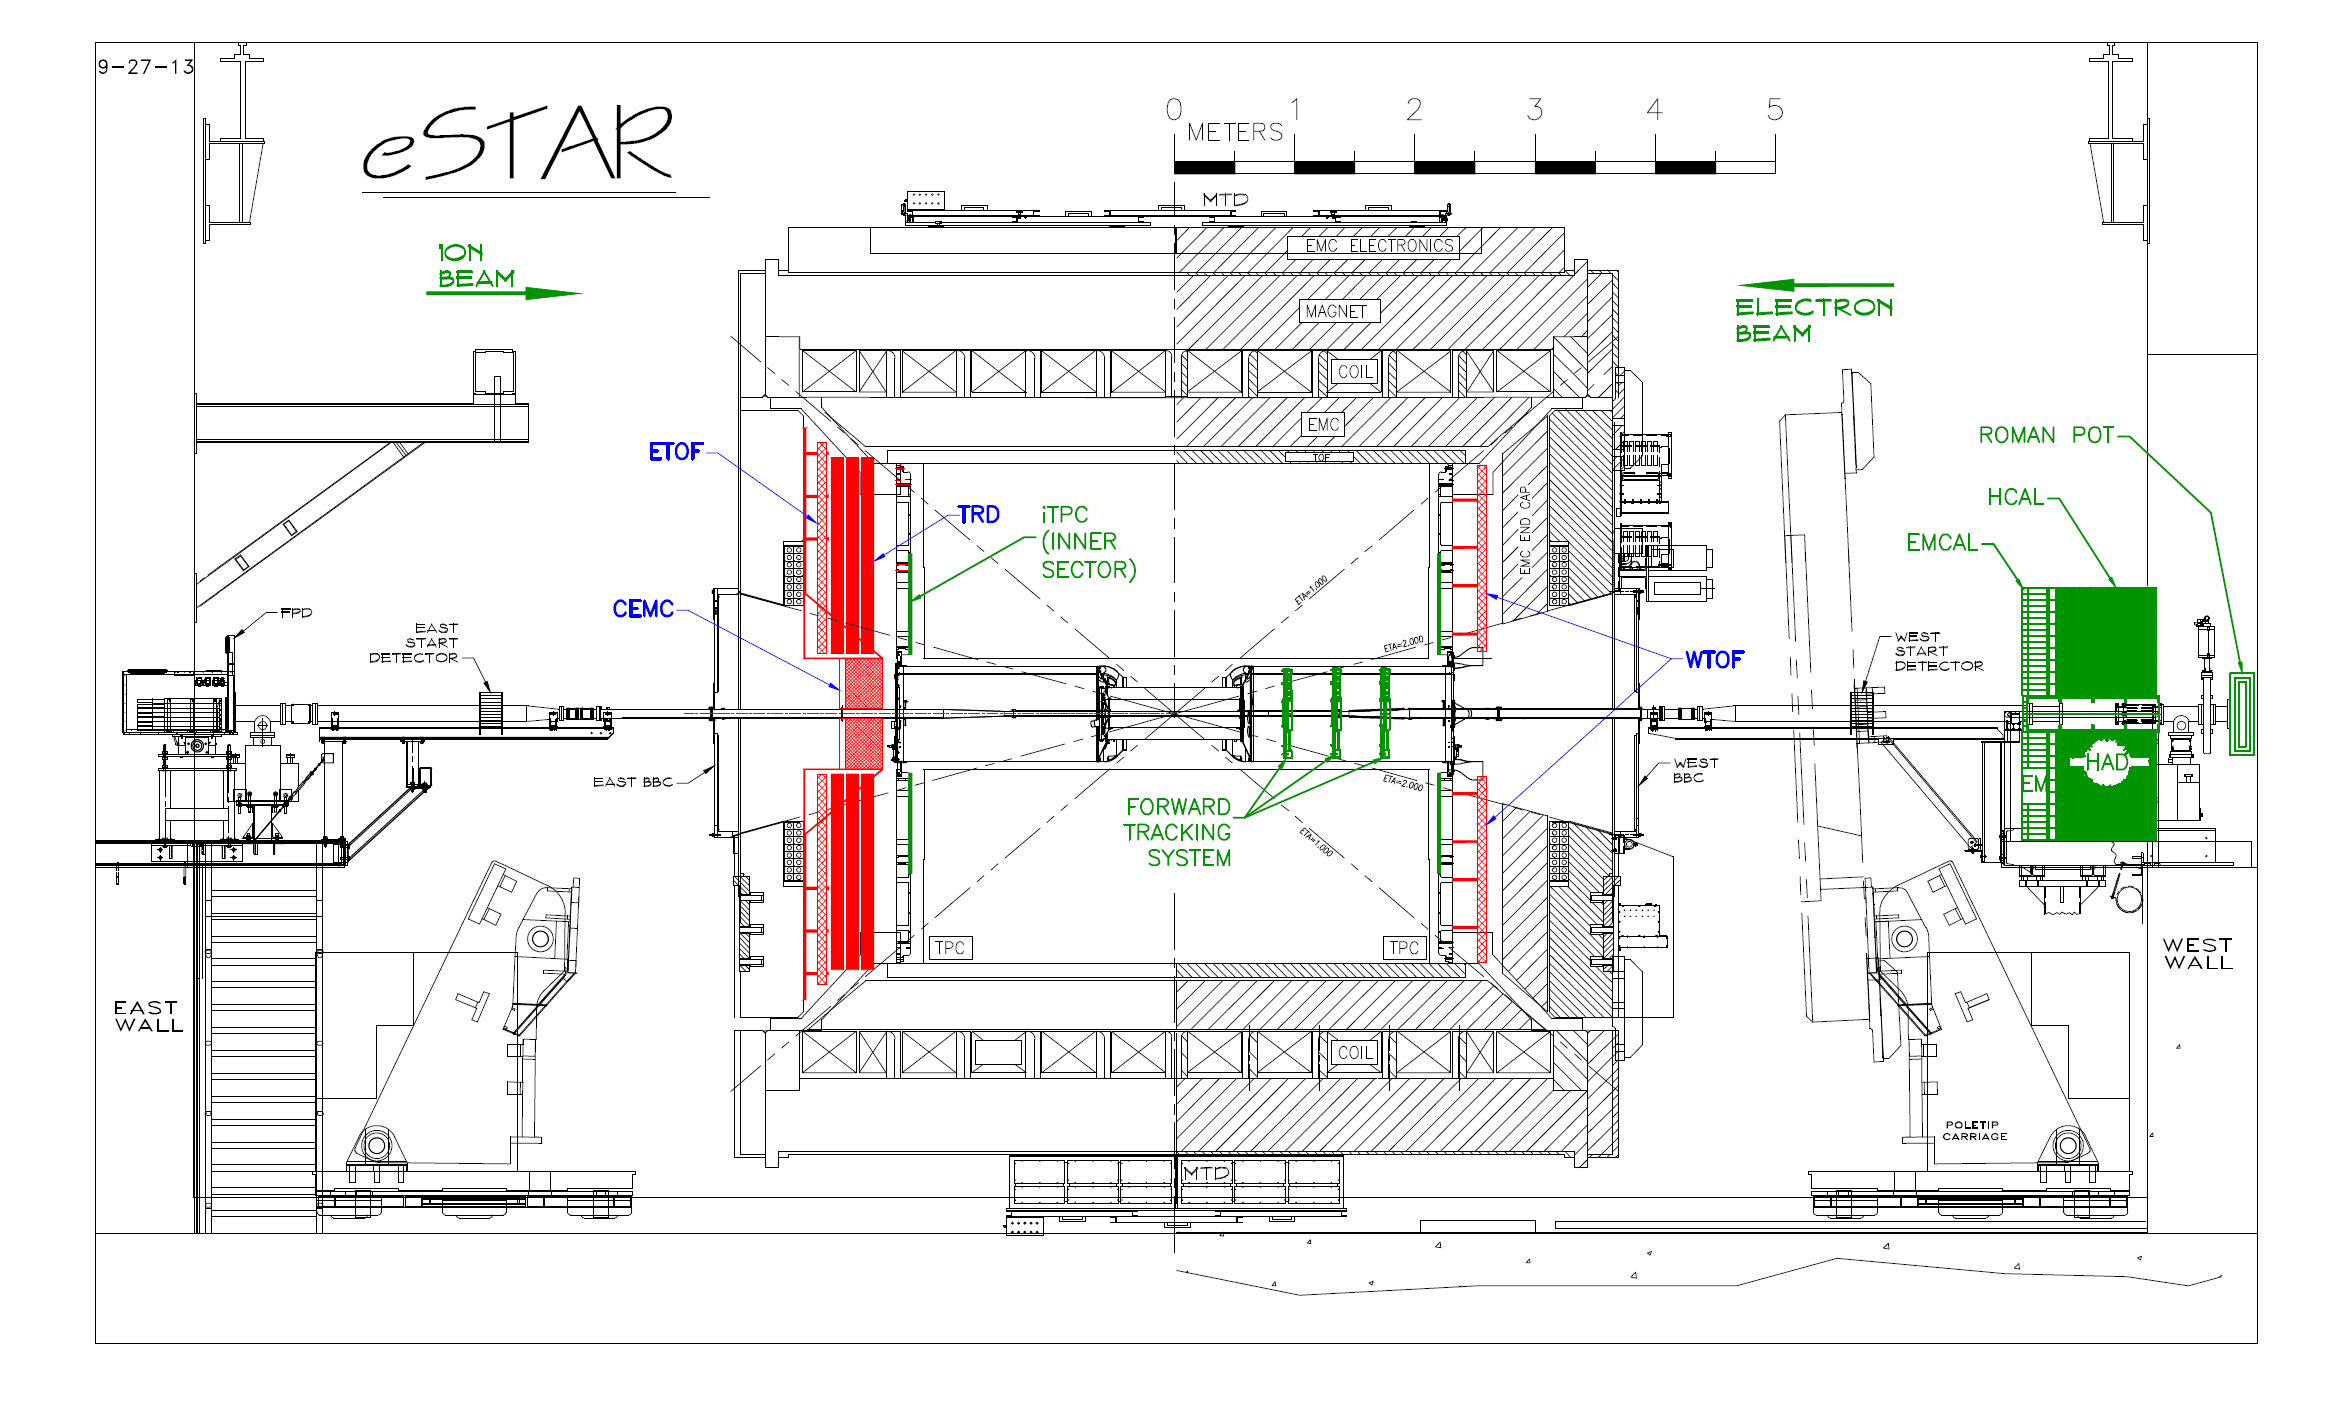
\includegraphics[width=0.8\textwidth]{plots/chpt4/eSTAR_layout.png}
\caption[Layout of eSTAR detector concept]{
eSTAR layout with proposed upgrades. Electron beam is from right to left while hadron beam is from let to right. The plot is Ref.~\cite{star_LoI}.}
\label{fig:eSTAR_layout}
\end{figure}

The proposed eSTAR detector configuration has been shown in
Fig.~\ref{fig:eSTAR_layout}. To identify the scattered lepton in $|\eta|>1$,
endcap TOF on both sides covering $1<|\eta|<2$ and GEM based TRD covering
$-2<\eta<-1$ will be added. Also, before the completion of RHIC program, a
forward tracking system with associated forward calorimeters will be installed.

The ePHENIX detector is going to reuse the superconducting solenoid and the
calorimeter system of sPHENIX, the proposed upgrade of PHENIX focusing on jet
physics. A possible layout has been shown in Fig.~\ref{fig:ePhenix_layout}.
Other than the reusable subsystems from sPHENIX, a few more new subsystems will
be added to the ePHENIX detector. The GEM detectors are needed in both electron
and hadron going direction, providing tracking information for the region
$|\eta|>1$. Endcap electromagnetic calorimeters will be equipped to have full
coverage over $-4<\eta<4$.
\begin{figure}
\centering
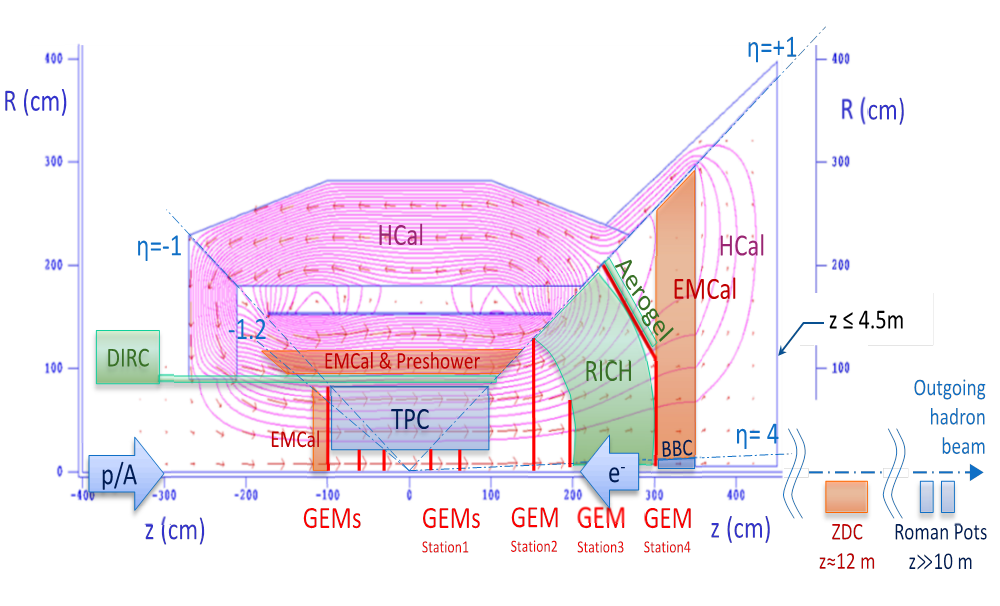
\includegraphics[width=0.8\textwidth]{plots/chpt4/ePhenix_layout.png}
\caption[Layout of ePHENIX detector concept]{
A cross view of the ePHENIX detector concept. The plot is Ref.~\cite{Adare:2014aaa}.}
\label{fig:ePhenix_layout}
\end{figure}


\chapter{Monte Carlo simulation method} \label{chp:MC}

In experimental particle physics, it is of great interest to use Monte Carlo
simulation method in designing detectors, understanding the detector responses
and comparing experimental data to theory predictions. In the work of this
thesis, we employ Monte Carlo simulation method for several reasons. First, we
need the simulated Monte Carlo event samples to determine if our current
designing detector parameters are good enough to characterize our targeted
measurement. As to the dihadron correlation measurement, it is the detector
coverage and resolution that we should take into consideration. Second, we will
rely on the Monte Carlo simulation method to evaluate the detector response
effect. Generally, this type of study is usually based on
GEANT~\cite{Brun:1978fy}. In our case, we use a simplified fast smearing method~\cite{EICsmear}.
In addition, we want to make some phenomenological predictions which are very
hard to be calculated with perturbative theory and can only be studied based on
some Monte Carlo models. In the end, with the event by event level description
of Monte Carlo generators we can estimate the statistical error, based on which
one can decide how much time it takes to make a conclusive measurement.

This chapter describes the Monte Carlo event generators we employed to simulate
physical events and also our fast smearing method used to estimate the detector response.


\section{The Monte Carlo event generator for \ep\ } \label{sec:MC_ep}
For the \ep\ collisions, we use the PYTHIA event generator~\cite{Sjostrand:2006za}. The event generation
process of PYTHIA can be summarized as follows (see Fig.~\ref{fig:PYTHIA_generation_scheme} for an example).
\begin{figure}
\centering
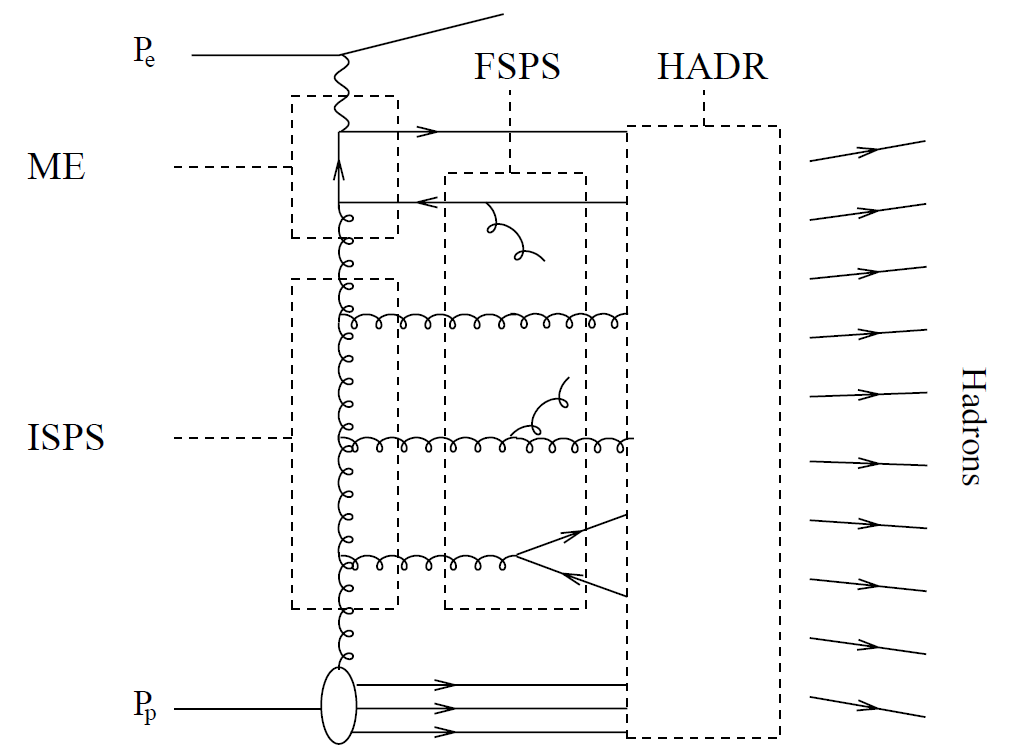
\includegraphics[width=0.7\textwidth]{plots/chpt5/PYTHIA_generation_scheme.png}
\caption[An illustration of the event generation process in PYTHIA] {
A schematic view of the event generation process in PYTHIA: hard scatering matrix element (ME), 
initial-state parton shower (ISPS), final-state parton shower (FSPS) and hadronization process (HADR). 
This plot is from Ref.~\cite{Hansson:2007zz} }
\label{fig:PYTHIA_generation_scheme}
\end{figure}
\begin{itemize}
\item Initial parton generations. The initial partons are generated depending
on the PDF description for the beam particles. The PDF sets are extracted from
a wide range of experimental tables with global fits method. It is further customary to assign a primordial transverse momentum to the initial partons, while the recoil is assumed to be taken by the beam particle remnants. 
\item Hard scattering process. The two initial partons from the beam particles may
have a hard interaction based on the matrix element for the specific Feynman diagram
determining the main kinematic feature of this event. For the PYTHIA generator, this
matrix element is calculated at the leading order.
\item Initial-state and final-state parton shower. In the parton shower model, partons
before and after hard scattering may have initial-state and final-state radiations, respectively. It
is an approximation to the higher-oder QCD process at the leading-log level. 
\item Hadronization and decay process. The generated final-state partons and
beam remnants will fragment into colorless hadrons, which is a non-perturbative process
and determined from the string model~\cite{Andersson:1983ia} in PYTHIA implementation. Unstable particles decay
until reaching a set of stable final-state hadrons.
\end{itemize}

The simulation part of this study is based on the PYTHIA-$6.4$ Monte Carlo program,
with the PDF input from the LHAPDF library~\cite{Whalley:2005nh} and JETSET string model used for
hadronization processes. 


The PYTHIA Monte Carlo generator is a general purpose Monte Carlo program developed to simulate a wide range of physics process. It can be well tuned to describe the data from various experiments. This is why we use PYTHIA for the simulation of \ep\ events.


\section{The Monte Carlo generator for \eA\ }

As is known to all, we have a rich set of \ep\ Monte Carlo event generators, but
unfortunately a less favorable case for \eA~\cite{Boer:2011fh}.
DPMJET~\cite{Roesler:2000he} is believed to be one powerful generator to fit
into the simulation task for \eA\ collisions. DPMJET is treating the eA
interaction based on individual photon nucleon events simulated by
PHOJET~\cite{Engel:1994vs} in Gribov-Glauber multiple scattering
formalism~\cite{Engel:1996yb}. In the individual photon nucleon interactions a
photon is assumed to be divided into a direct photon part and a hadronic part. The
description of hadronic photon on nucleon is based on the Generalized Vector
Dominance Model (GVDM). Direct photon events include Photon Gluon Fusion (PGF)
and QCD Compton (QCDC) process. A steady transition is allowed between direct
and hadronic photon events~\cite{Roesler:1998wy}. Meanwhile, we notice that
since PHOJET, the code responsible for the elementary interaction generation in
DPMJET, only describes the interaction involving photons at very low $Q^2$ ($Q^{2}\rightarrow 0$), which indicates 
this DPMJET code allows mainly the simulation of
photoproduction off nuclei. Clearly, for the study of saturation physics, we can not use a event generator
mainly developed to simulate photoproduction events. 

Considering the fact that PHOJET responsible for treating elementary photon
nucleon interaction is quite a standalone part in the whole DPMJET framework, it
occurs to us that if we can switch the part treating photon nucleon interaction
from PHOJET to some more multi-purposed package like
PYTHIA~\cite{Sjostrand:2006za}, we can largely enforce the ability and broaden
the applicable scope of DPMJET, for example to simulate the kinematics region
covered by a proposed EIC.

Within the flexible program design of PYTHIA, we are also allowed to implement
more features such as the nuclear PDF and energy loss effect in cold nuclear
matter to accommodate the non-saturation nuclear effect. 
With everything assembled together, we can build a hybrid Monte Carlo \eA\ generator reusing existing
code of DPMJET and PYTHIA at different levels with EPS09 nuclear PDF~\cite{Eskola:2009uj}
and the cold nuclear medium energy loss effect~\cite{Salgado:2003gb}. The physical process of an \eA\ collision is
generated as follows:

\begin{itemize}
    \item To begin with, a nucleon is sampled from the whole nucleus according to the nuclear geometry implemented in DPMJET.
    \item The elementary interaction of the incoming electron and the selected nucleon will be simulated according to the modules as described in PYTHIA (see Sec.~\ref{sec:MC_ep}).
    \item Before JETSET (the package responsible for parton fragmentation in PYTHIA) takes care of the final parton system in the last step, the parton energy loss effect in a cold nuclear medium will be performed to the hard scattering partons. 
    \item As we already have the particles generated for the elementary interaction from PYTHIA, we will will utilize DPMJET to simulate the intranuclear cascade process based on the generated DIS process information.
    \item To close it up, the FLUKA generator~\cite{Ferrari:1995cq} which already connected with DPMJET will be used to produce deexcitation photons, nuclear fragments and some heavy remnants from the broken nucleus.
\end{itemize}

\begin{figure}
\centering
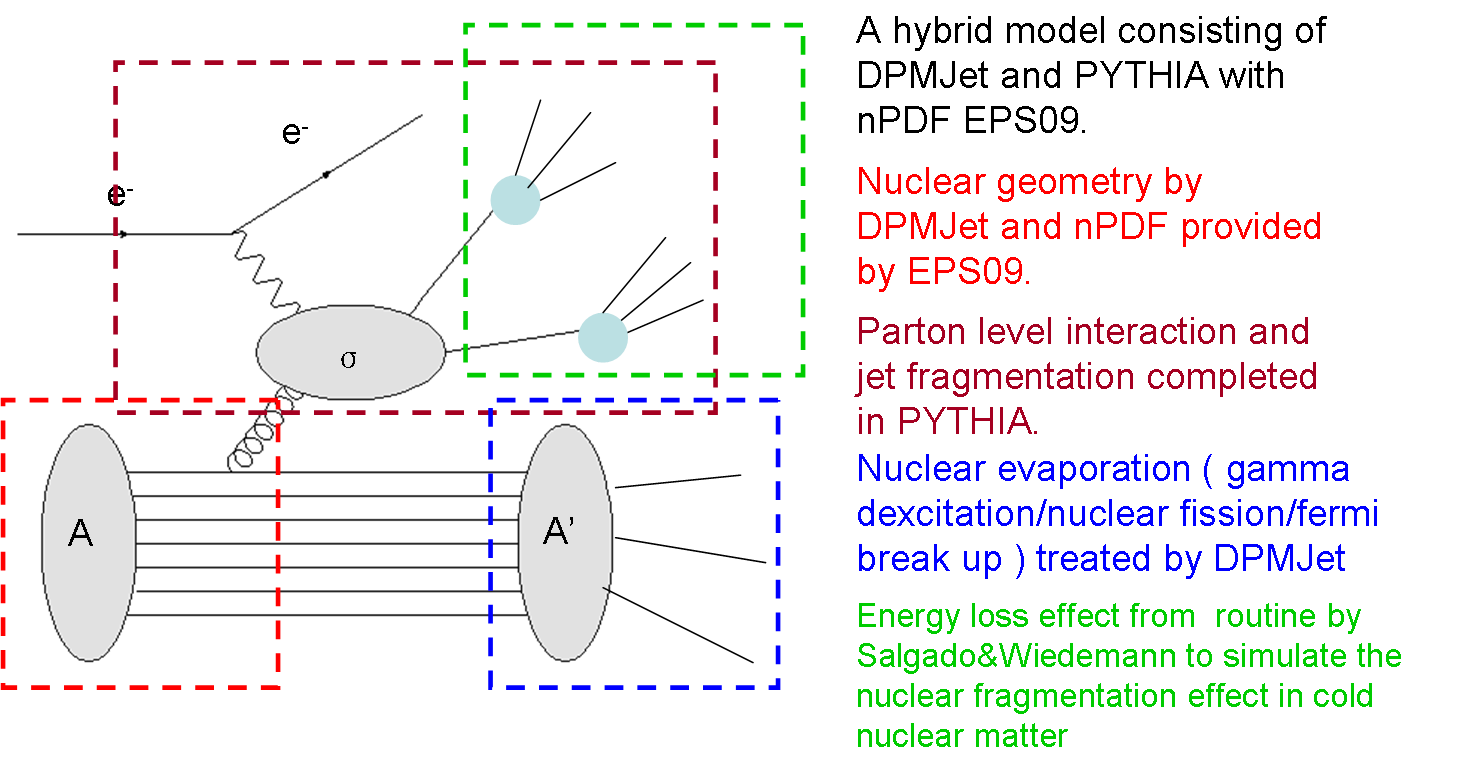
\includegraphics[width=1.0\textwidth]{plots/chpt5/eA_hybrid_chart.png} 
\caption[An illustration of the hybrid \eA\ Monte Carlo generator design layout] {
An illustration of the hybrid \eA\ Monte Carlo generator design layout. }
\label{fig:MC_hybrid_chart}
\end{figure}

The physical generation flow can be visualized in Fig.~\ref{fig:MC_hybrid_chart}.
In this model we have two significant non-saturation based nuclear effects implemented which are relevant to the dihadron correlation studies: the nuclear PDF and the cold nuclear medium energy loss effect.

\subsection{Nuclear parton distribution function}
In the hybrid Monte Carlo generator, we use a next-to-leading order (NLO) global
DGLAP analysis of nuclear parton distribution function (PDF) and their uncertainties with the release called
EPS09. Process independent PDFs of free and bound nucleons
have been discovered to be mutually different for well over twenty years. There
exist various groups offering parameterizations of the nuclear modified PDFs~\cite{Hirai:2004wq,deFlorian:2003qf}.


The nuclear modifications relative to the free nucleon PDFs are commonly named
according to the different x-regions as follows: (a) shadowing; a suppression at
$x\lesssim 0.1$, (b) antishadowing; excess around $0.1\lesssim x \lesssim 0.3$,
(c) EMC effect; depletion between $x\simeq 0.3$ and $x \simeq 0.7$, (d) Fermi
motion; an excess towards $x=1$. While the quark antiquark densities are
relatively well constrained, the modifications to gluon distributions are not
directly measured. Current nPDF parametrizations give wide variations in the
nuclear gluon densities especially in the small $x$ region due to the lack of the
nuclear DIS data in the corresponding region. However, hopefully with the advent
of the EIC era, the gluon density uncertainty can be largely constrained.

In the framework of EPS09 PDF analyses, nuclear PDF is defined with the following form
\begin{equation}
f^{A}_{i}(x, Q^{2}) \equiv R^{A}_{i}(x, Q^{2})f^{p}_{i}(x, Q^{2}),
\end{equation} 
where $R^{A}_{i}$ is the nuclear modification factor multiplied on top of the
free proton PDF $f^{p}_{i}(x, Q^{2})$ for a parton of flavor $i$, 
with $f^{p}_{i}(x, Q^{2})$ being the CTEQ6.1M PDF set. Figure.~\ref{fig:shadowing} shows an illustration of the function $R^{A}_{i}$. 
\begin{figure}
\centering
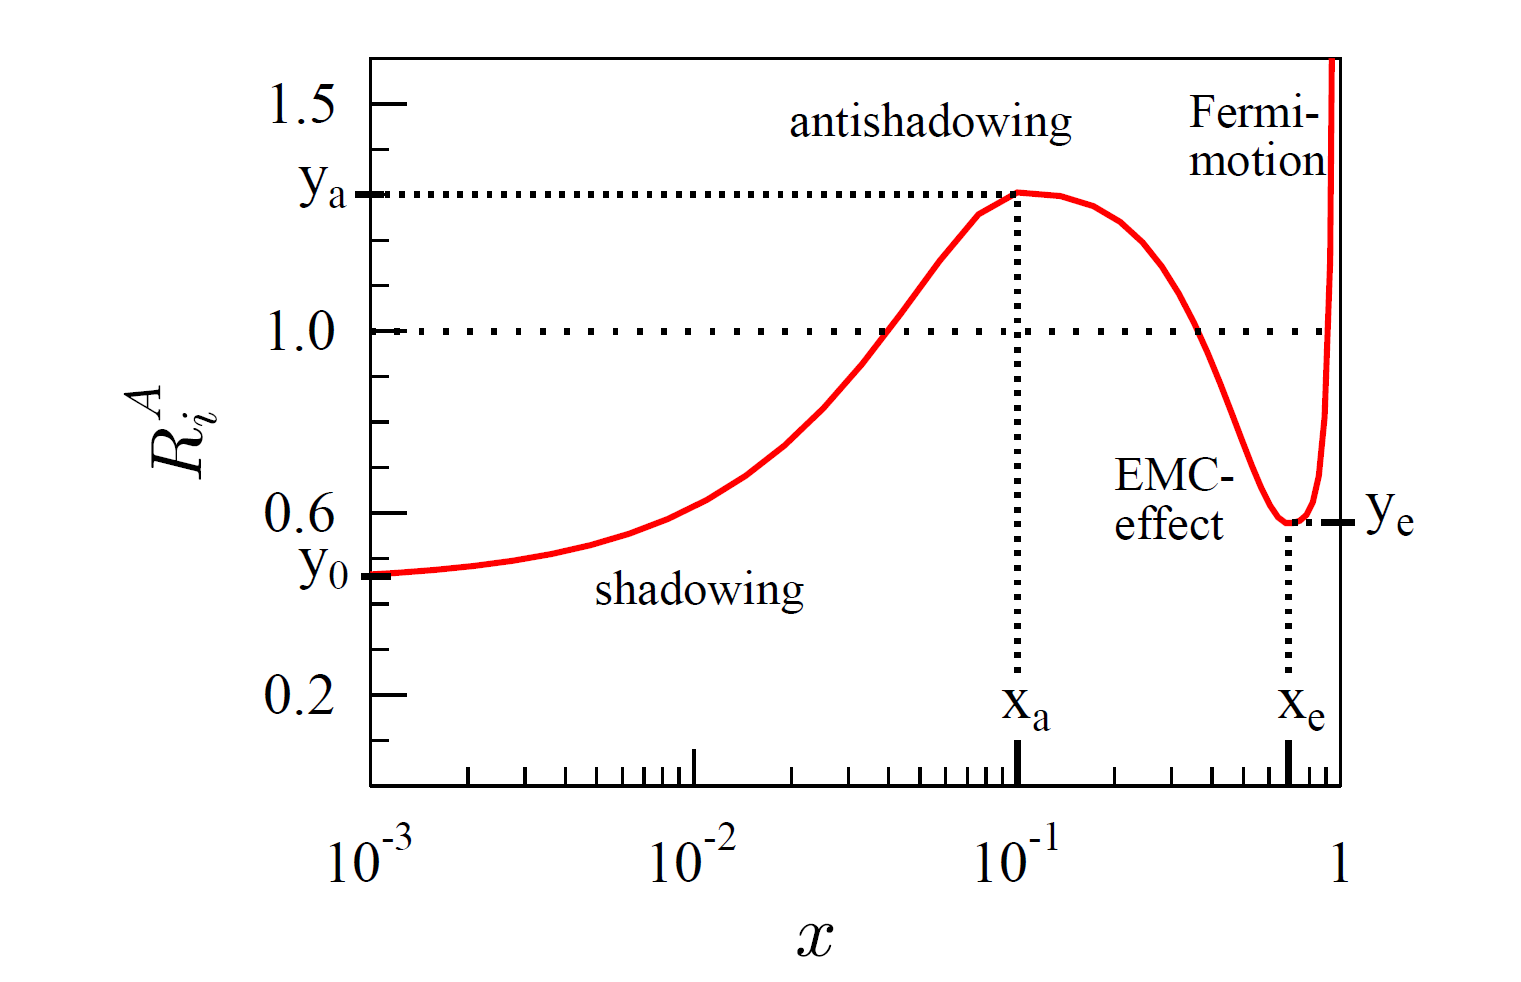
\includegraphics[width=1.0\textwidth]{plots/chpt5/shadowing.png} 
\caption[The plot showing the ratio of gluon distribution function in the nuclear medium divided by the proton gluon distribution function] {
An illustration of the function $R^{A}_{i}$. The plot is from \cite{Eskola:2009uj}.}
\label{fig:shadowing}
\end{figure}


Assuming isospin symmetry for protons and neutrons, the up/down quark
distribution can be obtained by average according to the corresponding mass
number $A$ and charge number $Z$.


\subsection{Parton energy loss in the cold nuclear medium } \label{sec:energy_loss}
The fragmentation is another piece needs to be modified by the nuclear effect
apart from that on the parton distribution function as in nuclear deep inelastic
scattering process. Because of the non-perturbative nature of hadronization, it
is impossible to be obtained directly from the first principle calculations. People have
to rely on the phenomenological models fitted to data to describe it. The models
are based on the following aspects: hadron absorption, parton energy loss and medium
modified fragmentation function. Hadron absorption models employ formation
times and absorption cross sections for the hadrons produced in the nuclear
environment, while parton energy loss models usually use QCD inspired
calculations characterizing gluon emission off highly virtual hard partons in
the nuclear environment.

In the hybrid Monte Carlo generator, a hard parton energy loss effect is
included following the Parton Quenching Model
implementation~\cite{Dupre:2011afa} based on the extended BDMPS
calculations~\cite{Salgado:2003gb}. The parton energy loss model is originally
focused on heavy ion collisions and the characterization of quark-gluon plasma
(QGP). But it can be easily transportable to the nuclear DIS case from which better
determined initial conditions can be extracted. Based on the knowledge
of the extracted initial conditions, a precise comparison with experiments
involving heavy ion collisions can be made to describe the formation of the QGP.

In the energy loss picture, a medium is described by its transport coefficient $\hat{q}$,
defined as the average medium induced transverse momentum square per unit path
length of a hard parton:
\begin{equation}
\hat{q} = \left\langle k^{2}_{\perp}\right\rangle _{medium}/\lambda,
\end{equation}
where $\lambda$ is the mean free path and $k_{\perp}$ denotes the transverse
momentum of the emitted gluon. The characteristic energy loss scale is set by:
\begin{equation}
\omega_{c} = \frac{1}{2}\hat{q}L^{2}.
\end{equation}
As the constraint on transverse momentum $k_{\perp}$ must be smaller than the
total energy, a dimensionless quantity $R$ is introduced:
\begin{equation}
R = \frac{2\omega^{2}_{c}}{\hat{q}L} = \omega_{c}L.
\end{equation}
$L$ is the path length that parton traverses in the medium, determined by the
coordinate of the nucleon involved in certain hard interaction sampled from
a Woods-Saxon nucleus geometry. To consider the nuclear medium geometry, all we
have to do is to average over the density profile of the matter traversed by the
parton. The probability for a parton to lose energy $\Delta E$ through $n$ gluon emissions can be
written as:
\begin{equation}
P(\Delta E)=\sum^{\infty}_{n=0}\frac{1}{n!}[\prod^{n}_{i=1}\int d\omega_{i}\frac{dI(\omega_{i})}{d\omega}]
\times(\Delta E-\sum^{n}_{i=1}\omega_{i})\exp[-\int d\omega\frac{dI}{d\omega}],
\end{equation}
where $\omega_{i}$ is the emitted gluon energy and the gluon energy spectrum
$\frac{dI}{d\omega}$ depends on the parameters we defined above. BDMPS formalism
gives results for $R\rightarrow \infty$ while Salgado and Wiedemann extended the
energy spectrum for moderate $R$ manifested by a suppression of small energy
gluon emission. The probability has a discrete part and a continuous part as
follows:
\begin{equation}
P(\Delta E) = p_{0}\delta(\Delta E) + p(\Delta E),
\end{equation}
where $p_{0}$ is the discrete probability that no medium induced radiation
happens to the parton.

In our simulation, the generation of energy loss iterates as:
\begin{itemize}
	\item generate an event list at parton level from the Monte Carlo package;
	\item determine two input parameters, $\omega_{c}$ and $R$ by the generated event information;
	\item sample an energy loss $\Delta E$ according to the $P(\Delta E)$ determined in the last step;
	\item dump the modified parton system to the JETSET fragmentation module, which gives us the final particle list.
\end{itemize}

%The transport coefficient is set to $\hat{q}=0.5$. And for the sake of
%simplicity, we only assign an energy loss to the longitudinal direction of a
%parton.
%

\section{EIC fast smearing package}


\begin{figure}
\centering
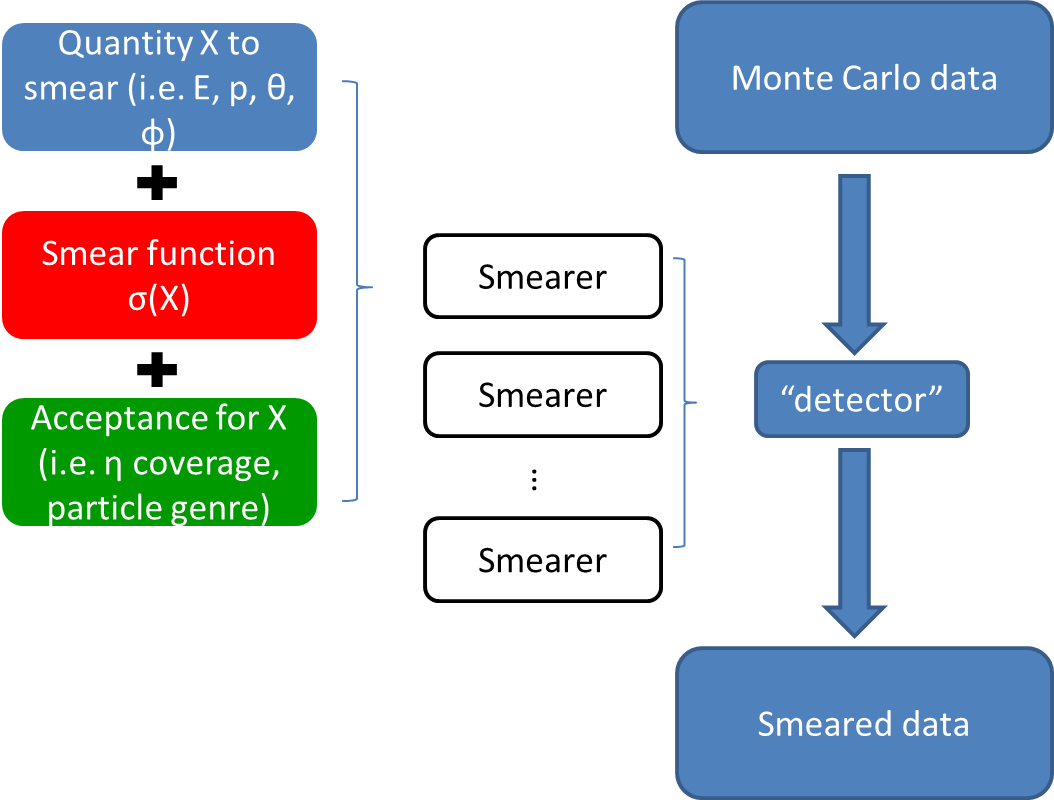
\includegraphics[width=0.8\textwidth]{plots/chpt5/smearing framework.png}
\caption[An illustration of the event smearing strategy in the eic-smear package] {
A schematic view of the event smearing process implemented in eic-smear package. 
}
\label{fig:smear_layout}
\end{figure}


When a detector system tracks a particle, the information of this particle
(momentum, energy, particle id, and so on) has to be reconstructed from the electronic
signals received and analyzed at the detector read out. How well the particle
information can be reconstructed or manifested at the detector read out is
estimated by the detector resolution. The detector with a better resolution
can reconstruct particle information closer to the true value. On
the other hand, to build a detector with very high resolution will cost a lot
of budget. To make the most cost-effective design, we need to know what kind
of detector resolution is good enough to manifest the targeting physical message.

The fast smearing method implemented in the eic-smear package is a systematic
way to study the effects of detector resolution economically. The eic-smear
package provides a means for applying detector smearing to the Monte Carlo
data, whereby kinematic properties from the Monte Carlo simulated particles are modified according
to a description of the detector performance. The package contains a series of
classes and functions to facilitate the smearing of ROOT trees created from
Monte Carlo event generator. It is intended to be extremely flexible,
allowing you to change what type of smearing you want to simulate quickly and
painlessly.

As implemented in eic-smear, it is much faster to run than a full detector
simulation (e.g. GEANT), both in terms of user time spent specifying the
detector properties and in CPU time spent processing events. However,  the
smearing code is not intended as a replacement for full detector simulations.
Rather, it is a complimentary tool for roughly assessing the impact of changes
in detector performance on a physics measurement, in a way that is much more
rapid, but less detailed, than a full detector simulation. It is designed to
answer questions like given a known detector resolution, how well can we
measure some physics variables. 

\begin{table} 
\centering 
\begin{tabular}{| l | c | c | } \hline
Device	& Acceptance & resolution \\ \hline
Barrel tracking  	&  $|\eta|<1.5$  &  $\sigma_{p}/p=0.1\%$   \\  
Endcap tracking    &  $1.5<|\eta|<3$  &   $\sigma_{p}/p=1\%$   \\  
ECal   & $-1<\eta<4.5$  &  $\sigma_{E}/E=12\%/\sqrt{E}$   \\  
ECal  & $-4.5<\eta<-1$ & $\sigma_{E}/E=1.8\%/\sqrt{E}$   \\ 
HCal  & $2<\eta<4.5$ & $\sigma_{E}/E=38\%/\sqrt{E}$   \\ \hline
\end{tabular} 
\caption[The
assumed resolution for the devices to be used in our dihadron correlation simulations]{The
assumed resolution for the devices to be used in our dihadron correlation simulations.}
\label{tab:EIC_smear} 
\end{table}


In this method, a virtual device ``smearer" is defined to smear a physical
quantity $X$ according to the user specified resolution if the particle is accepted
within the smearer's coverage as shown in Fig.~\ref{fig:smear_layout}. A smearer should not necessarily be considered to
be a direct analogue of a single real-world detector subsystem (though in some
cases it may be). Rather, it is a more abstract representation of some element
of the whole detector's performance. For example, while a user may define a
single device object for smearing momentum, this device may represent the
combined tracking performance and acceptance of a number of physical detector
subsystems.

We customized a simple smearing detector for our dihadron correlation
measurement based on the EIC model detector geometry setup. The assumed
resolutions for these devices are listed in Tab.~\ref{tab:EIC_smear}.





\chapter{Dihadron correlations at eRHIC}
\label{chp:dihadron}
As discussed in Chpt.~\ref{chp:saturation}, the dihadron correlation measurement
is a very compelling measurement to study the saturation effect. And there are
several advantages to perform this measurement at an EIC. It is of great
interest to measure dihadron correlations in \eA\ not only because it provides
complementary information to \dA\ or \pA\ but also because it is a unique and
clean means to probe the little known Weizs\"{a}cker-Williams (WW) gluon
distribution. The WW gluon distribution is an important and fundamental
unitegrated gluon distribution (UGD) existing in a lot of processes.

At the same time, to achieve an accurate description of experimental data it is
essential to have theoretical calculations beyond leading order, especially as
the higher-order corrections are known to be sizable. The analysis in this work
accounts for gluon radiation in the calculation of the dihadron cross section
through the inclusion of Sudakov factors. It is one of the most important
corrections computed on one-loop level. This is vital for the comparison between
the theory calculation and the future eRHIC data on dihadron correlations.

In the work of this chapter, based on the most recent theoretical developments in saturation
physics, we perform a detailed study of the feasibility, expected precision, and
physics impact of dihadron correlation measurements on gluon dynamics in the
small $x$ region at a future high-luminosity, high-energy EIC. We will
demonstrate that, at the future eRHIC, it is feasible to perform the discussed
dihadron correlation measurement even with a moderate integrated luminosity of
$\mathcal{L}=1 \, fb^{-1}$. We present results for two lepton-nucleus beam energy
configurations, 10 GeV $\times$ 100 GeV and 20 GeV $\times$ 100 GeV, and compare
the results for proton and gold beams. We use pseudo-data generated by the Monte
Carlo event generator PYTHIA (as mentioned in Chpt.~\ref{chp:MC}) integrated with nuclear PDFs,
geometry and energy loss to obtain a non-saturation baseline. The framework of
Ref.~\cite{Dominguez:2011wm} is used to obtain numerical predictions and to
study the size of the suppression of dihadron correlations in a saturation
formalism.


The rest of this chapter is organized as follows: in
Sec.~\ref{sec:dihadrontheory}, we discuss the theoretical framework used for the
prediction of saturation effects in the dihadron correlation measurement. A
brief comparison of dihadron correlations in \eA\ versus \pA\ is provided in
Sec.~\ref{sec:dihadroneAvspA}. We discuss our simulation work based on a
nonsaturation Monte Carlo model in Sec.~\ref{sec:dihadron_nonsat_mc} and the
results in the followed sections. Finally, we summarize and conclude in
Sec.~\ref{sec:dihadronsummary}.




\section{Dihadron correlations in the saturation Formalism}\label{sec:dihadrontheory}

According to the effective small-$x$ $k_T$ factorization established in
Ref.~\cite{Dominguez:2011wm}, which is briefly summarized above, the
back-to-back correlation limit of the dihadron production cross section can be used
to directly probe the WW gluon distribution $xG^{(1)}(x,q_{\perp})$. As a
comparison, the hadron production in semi-inclusive deep inelastic scattering
(SIDIS), as shown in Ref.~\cite{Marquet:2009ca}, is related to the so-called
dipole gluon distributions $xG^{(2)}(x,q_{\perp})$.

The coincidence probability $C(\Delta\phi)=\frac{N_{pair}(\Delta\phi)}{N_{trig}}$ is a
commonly exploited observable in dihadron correlation studies, in which
$N_{pair}(\Delta\phi)$ is the yield of the correlated trigger and associate
particle pairs, while $N_{trig}$ is the trigger particle yield. This
correlation function $C(\Delta\phi)$ depends on the azimuthal angle difference $\Delta\phi$
between the trigger and associate particles. In terms of theoretical
calculation, the correlation function is defined as
\begin{eqnarray} 
C(\Delta\phi) 
= & \frac{1}{\frac{d\sigma^{\gamma^{*}+A\rightarrow h_{1}+X}_{\textrm{SIDIS}}}{dz_{h1}}}
\frac{d\sigma^{\gammaA}_{\textrm{tot}}}{dz_{h1}dz_{h2}d\Delta\phi}.
\label{eqn:cdphiCGC} 
\end{eqnarray}

Let us consider a process of a virtual photon scattering on a dense nuclear target
producing two final state back-to-back $q\bar q$ jets:
$\gamma^{*}+A\rightarrow q(k_{1})+\bar{q}(k_{2})+X$, in which $k_1$ and $k_2$ are
the four momenta of the two outgoing quarks. This process is the
dominant one in the low-$x$ region, since the gluon distribution is much larger than
the quark distributions inside a hadron at high energy. The back-to-back correlation
limit indicates that the transverse momentum imbalance is much smaller than each
individual momentum: $q_{\perp}=|k_{1\perp}+k_{2\perp}|\ll P_{\perp}$, with
$P_{\perp}$ defined as $(k_{1\perp}-k_{2\perp})/2$. At leading order (LO), the
dihadron total cross section, which includes both the longitudinal and
transverse contributions, can be written as follows~\cite{Dominguez:2011wm}:

\begin{eqnarray}\label{eqn:xspairCGC}
\frac{d\sigma^{\gammaA}_{\textrm{tot}}}{\phase} = & C\int^{1-z_{h2}}_{z_{h1}} dz_{q}
\frac{z_{q}(1-z_{q})}{z^{2}_{h2}z^{2}_{h1}}
d^{2}p_{1\perp}d^{2}p_{2\perp}\mathcal{F}(x_{g},q_{\perp})
\mathcal{H}_{\textrm{tot}}(z_{q},k_{1\perp},k_{2\perp}) \\ \nonumber
& \times \sum_{q}e^{2}_{q}D_{q}(\frac{z_{h1}}{z_{q}},p_{1\perp})
D_{\bar{q}}(\frac{z_{h2}}{1-z_{q}},p_{2\perp}),
\end{eqnarray}  
where $C=\frac{S_{\perp}N_{c}\alpha_{em}}{2\pi^{2}}$ gives the normalization
factor, with $S_{\perp}$ being the transverse area of the target, $z_{q}$ is the
longitudinal momentum fraction of the produced quark with respect to the incoming
virtual photon, $\mathcal{H}_{\textrm{tot}}$ is the combined hard factor,
$k_{1\perp}$ and $k_{2\perp}$ are the transverse momenta of the two quarks, while
$p_{h1\perp}$ and $p_{h2\perp}$ are the transverse momenta of the two corresponding
produced hadrons respectively. $\mathcal{F}(x_{g},q_{\perp})$ comes from the
relevant WW gluon distribution $xG^{(1)}(x_g,q_\perp)$ evaluated with the gauge
links for a large nucleus at small $x$ by using the McLerran-Venugopalan
model~\cite{McLerran:1993ni},
\begin{equation} 
\mathcal{F}(x_{g}, q_{\perp}) =
\frac{1}{2\pi^{2}} \int d^{2}r_{\perp} e^{-iq_{\perp}r_{\perp}}
\frac{1}{r^{2}_{\perp}}[1-\exp(-\frac{1}{4}r^{2}_{\perp}Q^{2}_{s})],
\end{equation}
in which $x_{g}=\frac{z_{q}p_{h1\perp}^2}{z_{h1}^2s}+\frac{(1-z_{q})p_{h2\perp}^2}{z_{h2}^2s}+\frac{Q^2}{s}$ 
is the longitudinal momentum fraction of the small-$x$ gluon with respect to the target hadron and 
$Q_{s}$ is the gluon saturation scale. $D_{q}(\frac{z_{h}}{z_{q}},p_{\perp})$ represents the transverse 
momentum dependent fragmentation functions, where $p_{\perp}$ shows the additional transverse
momentum introduced by fragmentation processes.

In principle, the so-called linearly polarised gluon
distribution~\cite{Metz:2011wb,Dominguez:2011br} also contributes to the dihadron
correlation and can be systematically taken into account. This part of the
contribution comes from an averaged quantum interference between a scattering
amplitude and a complex conjugate amplitude with active gluons linearly
polarized in two orthogonal directions in the azimuthal plane. Numerical
calculation shows that this contribution is negligible for dihadron back-to-back
correlations. Also, this type of contribution vanishes when the dihadron correlation function 
is averaged over the azimuthal angle of the trigger particle. 


As to the single-inclusive-hadron production cross section, which enters the
denominator of the definition of the correlation function $C(\Delta\phi)$, it
can be calculated from the saturation physics/CGC formalism~\cite{Marquet:2009ca} as
follows:
\begin{eqnarray}\label{eqn:xstrigCGC}
\frac{d\sigma^{\gamma^{*}+A\rightarrow h_{1}+X}_{\textrm{SIDIS}}}{dz_{h1}d^{2}p_{h1\perp}} 
= & C \int^{1}_{z_{h1}}dz_{q} \int
d^{2}q_{\perp}F_{x_{g}}(q_{\perp})H_{\textrm{SIDIS}}(k_{\perp},q_{\perp},Q) \\ \nonumber
  & \times \sum_{q} e^{2}_{q}\frac{z_{q}}{z^{2}_{h1}}D_{q}(\frac{z_{h1}}{z_{q}}),
\end{eqnarray}
where $H_{\textrm{SIDIS}}$ is the $q_{\perp}$ dependent hard factor for SIDIS,
which includes both the longitudinal and transverse photon contribution. Here
$F_{x_{g}}(q_\perp)$, which is related to $xG^{2}(x_g,q_\perp)$, is the Fourier
transform of the dipole cross section:
\begin{eqnarray}
F_{x_{g}}(q_{\perp})& = &\int \frac{d^{2}r}{2\pi^{2}}e^{iq_{\perp}\cdot
r_{\perp}} \frac{1}{N_{c}} Tr\langle
U(r_{\perp})U^{\dag}(0)\rangle_{\rho} \\ \nonumber
& \simeq &\frac{1}{\pi
Q^{2}_{sA}}\exp[-\frac{q_{\perp}^{2}}{Q^{2}_{sA}}]. 
\end{eqnarray}
It has been suggested in Refs~\cite{Dominguez:2011gc, Dumitru:2011vk} that both
dipole and WW gluon distributions have similar geometric scaling behavior.
Therefore, one can parameterize these gluon distributions following the
Golec-Biernat W\"{u}sthoff (GBW)~\cite{GolecBiernat:1998js} model calculation, in
which $Q^{2}_{sA}(x)=c(b)A^{1/3}Q^{2}_{s0}(x/x_{0})^{-\lambda}$, with $Q_{s0}=1$
GeV, $x_{0}=3.04\times 10^{-4}$ and  $\lambda=0.288$. The gluon saturation
momentum is related to $Q^{2}_{sA}(x)$ by
$Q_s^2(x)=\frac{2N_c^2}{N_c^2-1}Q^{2}_{sA}(x)$. $c(b)=c(0)\sqrt{1-b^{2}/R^{2}}$
gives the nuclear profile dependence with a radius $R$, where $b$ is the impact
parameter. As it is not an easy task to determine the exact impact parameter in \eA\
collisions, a median number $c(b)=0.8$ is used for the estimation,
which is supposed to average the nucleus geometry effectively. The parametrized
DSS fragmentation function~\cite{deFlorian:2007aj},
$D(z,p_{\perp})=D(z)\frac{1}{\pi\langle
p^{2}_{\perp}\rangle}e^{\frac{-p_{\perp}^{2}}{\langle p^{2}_{\perp}\rangle}}$ with
$\langle p^{2}_{\perp}\rangle=0.2 \, \mathrm{GeV}^{2}$, is used to compute the hadron
production.

By utilizing Eq.~(\ref{eqn:xspairCGC}) and Eq.~(\ref{eqn:xstrigCGC}), one can
straightforwardly calculate the coincidence probability. The theoretical
prediction at the Born level for the suppression of the away-side of the
dihadron correlation measurement is shown by the solid curves in
Fig.~\ref{fig:dihadron_theory_sud}.

All the above results are estimated based on the LO Born level
contribution. At the EIC energy scale the one-loop
contribution~\cite{Mueller:2012uf}, which is also known as the so-called Sudakov
factor, can be important as well. To include the Sudakov factor contribution at
leading double logarithm level, one can rewrite the relevant WW distribution as
follows~\cite{Mueller:2013wwa}:
\begin{equation}
\mathcal{F}(x_{g}, q_{\perp}) =
\frac{1}{2\pi^{2}} \int d^{2}r_{\perp} e^{-iq_{\perp}r_{\perp}}
\frac{1}{r^{2}_{\perp}}[1-\exp(-\frac{1}{4}r^{2}_{\perp}Q^{2}_{s})]
\exp[-\frac{\alpha_sN_c}{4\pi}\ln^2\frac{K^2r_{\perp}^2}{c^2_0}],
\label{eqn:Sudakov}
\end{equation}
where $K^2$ represents the hard momentum scale in two-particle production
processes. It can be chosen as $K^2=P^2_{\perp}$ or $K^2=Q^2$, depending on which
one is larger, and $c_0=2e^{-\gamma_E}$ with the Euler constant $\gamma_E$. It
is known that the single logarithmic terms as well as the next-to-leading order
(NLO) contribution of the Sudakov factor also have sizeable contributions 
compared to the above leading double logarithmic contribution. Therefore, the
numerical value of $\alpha_s$ in the Sudakov factor used in this calculation may
be different from what one normally expects according to a QCD running coupling
constant calculation.

One needs to pay attention to the applicability of this calculation.
As the GBW model is not sufficient to describe the UGDs in the region where 
$q_{\perp}$ is much larger than $Q_s$, we should limit this calculation to the
saturation region ($x_g<0.01$) to ensure the GBW model
can be applied. Additionally, to ensure that the power corrections to the
two-particle production are negligible, one needs the magnitude of the jet
transverse momenta $P_{\perp}$ to be much larger than $Q_s$.

The current calculations are performed for $Q^2$ of the same order as
$P^2_{\perp}$. For pair production, the Sudakov factor is usually due to
a scale difference between $P_{\perp}$ and the dijet momentum imbalance $q_{\perp}$.
Because we have required that $P_{\perp}\gg q_{\perp}$ as discussed above, it is
necessary to include the Sudakov contribution.  As for the trigger hadron
inclusive cross section, the Sudakov factor is not important, since the trigger
hadron \pt is of the same order as $Q$ and $P_\perp$. An illustration of
this Sudakov effect with $\alpha_s=0.35$ can be found in
Fig.~\ref{fig:dihadron_theory_sud} labeled by the dashed lines.
\begin{figure}
\centering
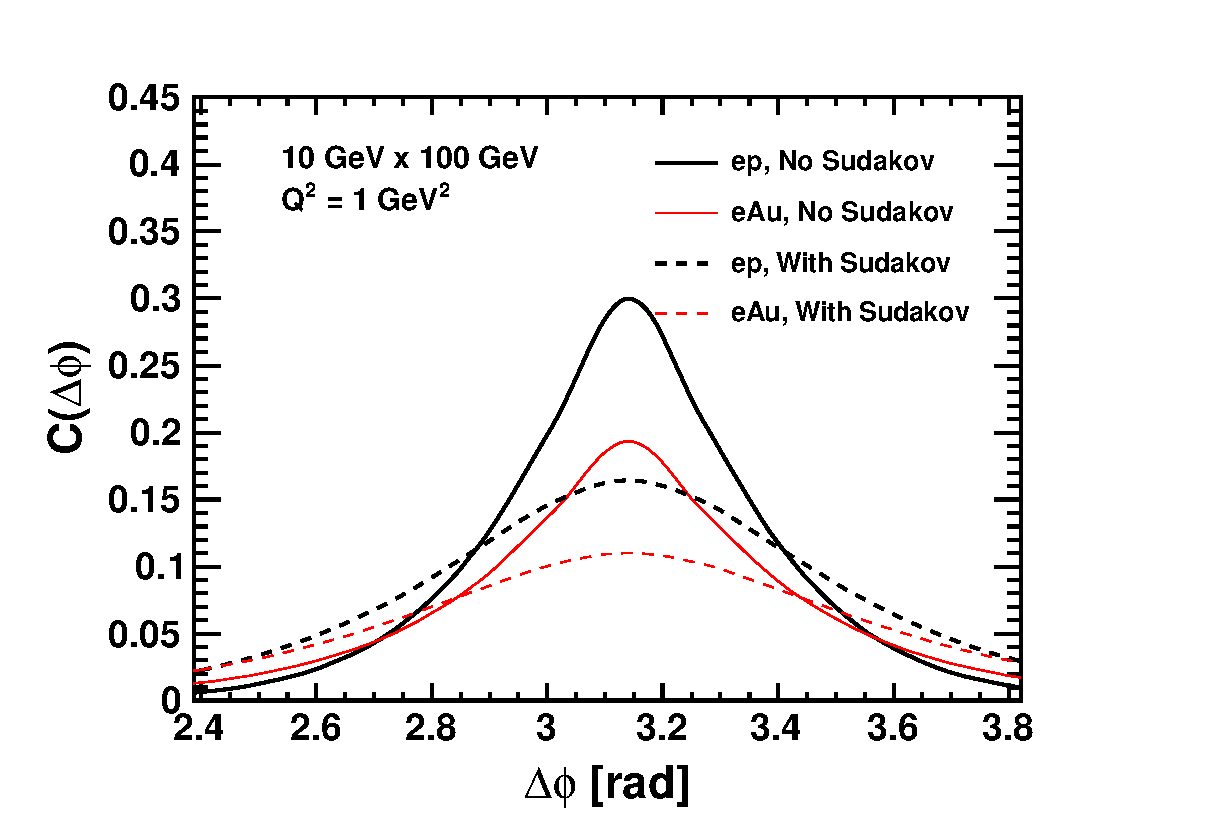
\includegraphics[width=0.7\textwidth]{plots/chpt6/theory_10x100_y_0.7_deltaphi_Sud_as_0.35.eps} 
\caption[theory prediction of dihadron correlation with Sudakov] {
$\pi^0$-correlation curves calculated in the saturation formalism at 10
GeV$\times $100 GeV for \ep\ (thick line) and \eAu\ (thin line) with (dashed
curve) and without (solid curve) the Sudakov factor. The kinematics chosen are
$y=0.7$, $Q^2=1 \, \textrm{GeV}^2$, $z_{h1}=z_{h2}=0.3$, $p_{h1\perp}>2 \,
\mathrm{GeV}/c,1 \, \mathrm{GeV}/c<p_{h2\perp}<p_{h1\perp}$.
\label{fig:dihadron_theory_sud}
}    
\end{figure}
It is worthwhile to point out that the Sudakov effect in a nuclear environment
is still not very well known. In the current small $x$ scenario as shown in
Eq.~(\ref{eqn:Sudakov}), it is convoluted with the gluon distribution function.
The theoretical calculation indicates that the Sudakov factor has no nuclear
$A$ dependence at LO. As shown in Fig.~\ref{fig:dihadron_theory_sud}, the away-side 
suppression of the dihadron correlation is due to the combination of the
Sudakov suppression and saturation effects. It is conceivable that the
suppression due to saturation effects shall become more and more dominant when
the ion beam species are changed from proton to gold, while the Sudakov effect
remains more or less the same. 

%The kinematic variables are defined
%as $Q^{2}=-q^{2}$, $y=\frac{P\cdot q}{P\cdot k}$, $z_{h}=\frac{P\cdot
%P_{h}}{P\cdot q}$ where $P_{h}, k, P$ and $q$ are the 4-momenta of the final state
%hadron, incoming lepton and nucleon (nucleus) and the exchanged photon. $p_{1T}$ and
%$p_{2T}$ are the transverse momenta with respect to the virtual photon for
%trigger and associate particle, respectively. Accordingly, $z_{1h}$ and $z_{2h}$
%are the $z_{h}$ for trigger/associate particles. 

\subsection{Connections to \pA\ dihadron correlations}\label{sec:dihadroneAvspA}

Compared to existing \pA\ or \dA\ dihadron correlation data, there are
several advantages to measuring dihadron correlations in \eA\ collisions. 
One valuable feature is that one can make use of the scattered electron to
reconstruct kinematic information event by event. Measuring
the scattered electron allows us to model-independently determine the required
kinematic variables $x$ and $Q^{2}$, which is essential for probing the
underlying gluon dynamics precisely. Another advantage comes from the point-like
structure of electrons. Since electrons have no substructure and they couple to
virtual photons rather weakly, the probability to have multiple emission in \eA\
is very small compared to \pA. This kind of multiple emission or
interaction introduces a significant amount of uncorrelated two-particle production,
which is known as the ``pedestal'' effect in RHIC \dA\ collisions. To understand the
so-called pedestal effect, one needs to take into account the double parton
scattering, which includes two independent and uncorrelated hard scatterings. In
contrast, as explained above, the pedestal contribution should be negligible and
under control in the \eA\ dihadron correlation measurement.

In addition, as is shown in Fig~\ref{fig:eAvspA_kinematics}, the kinematic
coverage of the planned eRHIC realization of the EIC
is very similar to the measured RHIC \dA\ data and
extends to the desired small-$x$ region. Therefore, it will be a more precise and definite
measurement compared to what we already know from the RHIC \dA\ data.
Here, the RHIC kinematics lines are calculated with the assumption that the major fraction of 
the parton energy is mainly taken by the hadrons, which is not always true.


\begin{figure}[hbt] 
\begin{center}
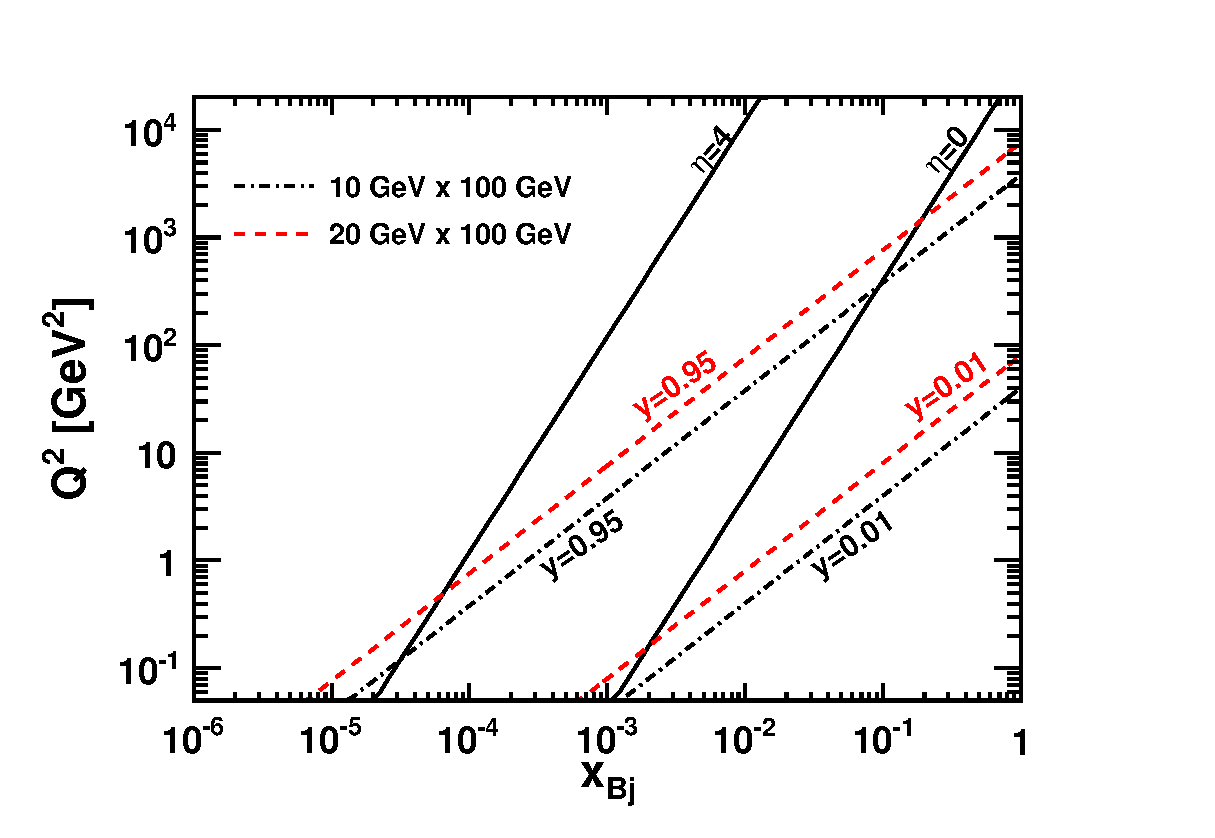
\includegraphics[width=0.7\textwidth]{plots/chpt6/eAvsdA_kinematics.eps} 
\end{center} 
\caption[kinematics coverage of eRHIC vs RHIC]
{The eRHIC kinematics coverage compared to \pA\ at RHIC. The dash-dotted and dashed
lines show the eRHIC kinematics for the beam energies of 10 GeV
$\times$100 GeV and 20 GeV $\times$100 GeV, respectively. The solid lines 
represent the RHIC coverage at $\sqrt{s}=200$ GeV for $\eta=0$ and $\eta=4$, where
$\eta=-\ln\tan(\theta/2)$ is the pseudorapidity of the particles.
\label{fig:eAvspA_kinematics}}
\end{figure}

The measurement of dihadron correlations in \eA\ collisions is
interesting by itself. It provides us with a golden opportunity to directly
measure the saturated WW gluon distribution. Through detailed calculations,
Ref.~\cite{Dominguez:2011wm} summarizes the involvement of these two basic
gluon distributions in different observables. It is interesting
to note that the dipole gluon distribution function is involved in most
known processes, especially inclusive DIS measurements, which provides us with a
lot of the essential information of the dipole scattering amplitude. On the
other hand, the WW gluon distribution contributes to only a few of these
processes, thus very little knowledge about the WW distribution exists from
the current experimental data. In addition, unlike the dijet process in \pA,
which receives contribution from both the dipole and WW gluon distribution, the WW gluon
distribution is the only UGD that contributes to \eA\ Dijet production. Considering
that the WW gluon distribution can be physically interpreted as the number density
of gluons inside a nuclear wave function, while the dipole gluon distribution
does not have such interpretation, it is important and fundamental to
acquire direct information on the WW gluon distribution through dihadron
correlation measurements at an EIC.



\section{Dihadron correlations in the nonsaturation model} \label{sec:dihadron_nonsat_mc}

If one defines $\hat{p_{T}}$ as the transverse momentum
of final state partons in the center of mass system of the hard interaction, the
factorization scale $\mu^{2}$ of $2\rightarrow 2$ processes can be expressed
as $\mu^{2} = \hat{p_{T}}^{2} + \frac{1}{2}Q^{2}$.


To simulate \ep\ events the CTEQ6M~\cite{Pumplin:2002vw} PDF in the
$\overline{\textrm{MS}}$ scheme is used. For the \eA\ event sample, the NLO
EPS09 parton distribution functions \cite{Eskola:2009uj} and hard parton energy
loss based on the medium geometry have been applied to account for nuclear
effects in the simulation. 
The hard parton energy loss in the nuclear medium is included
following the parton quenching model (PQM) formalism based on
Ref~\cite{Salgado:2003gb}.
In the phenomenological studies of dihadron correlations, triggering on a hadron
with high-$p_T$ on average selects the most energetic hadron in events with 
back-to-back jets. Correlated hadron pairs reflect two important features of QCD 
dynamics of the hard scattering process.
First, an associated hadron at the near-side allows one to probe the in-medium
QCD evolution of an energetic parton, which can be viewed as the final state
effect with the nuclear medium. Second, an associated hadron at the away-side,
in addition to the primary hard scattering, is sensitive to the initial
transverse momentum that the incoming parton carries.

For pQCD calculations in the collinear factorization framework, the PDFs and fragmentation
functions do not contain any transverse momentum dependence. Therefore, the
transverse momentum of hadrons produced in the final state is given by
$p_{T}=z\hat{p_{T}}$, where $\hat{p_{T}}$ and $p_{T}$ are the transverse
momentum of the parton and hadron respectively. $z$ represents the momentum fraction
of a hadron with respect to its mother parton. This relation should be revised
if the transverse momentum is allowed in both the PDFs and fragmentation
functions.

Transverse motion of partons inside hadrons can be effectively included by
assuming that the intrinsic \kt follows a Gaussian distribution. Similarly, the
transverse momentum enhancement  $p_{T}^{\textrm{frag}}$ with respect to the jet
direction during hadronization can also be approximated by a Gaussian
distribution. The intrinsic \kt and fragmentation $p_{T}^{\textrm{frag}}$ now
both contribute to the transverse momentum of final state hadrons, which can be
written as $p_{T} =z(k_{T}+\hat{p_{T}})+p_{T}^{\textrm{frag}}$. We follow the
common practice to set the Gaussian width to $0.4$ GeV for both intrinsic $k_{T}$ 
and $p_{T}^{\textrm{frag}}$ distributions in the simulations.

Besides all the above effects, additional soft gluon radiations, normally 
characterized as a parton shower can also modify the final transverse
momentum, thereby impacting the dihadron correlations. In perturbative QCD
calculations the parton shower are computed in terms of Sudakov
form factors.

Fig.~\ref{fig:dihadron_effects} shows an illustration of all the possible
effects available in the Monte Carlo in the simulation of the azimuthal correlation
function. The open circles illustrate the dihadron correlation with only
intrinsic $k_T$ in the initial parton distribution. It is understandable that the
correlation function is strongly peaked at $\Delta \phi =0, \pi$ for this setting.
Now the other effects are turned on one-by-one according to the order of their
occurrences in physical processes. When the initial state (IS) parton shower
is added into the simulation, as shown by the open diamonds, the away-side
correlation is significantly reduced since it is very sensitive to the momentum
imbalance of the dijet system, while the near-side correlation is almost
unmodified. Next, we turn on the final state (FS) parton shower for the scattered 
parton before the fragmentation process occurs. We find that both the
near-side and away-side peaks are broadened, as illustrated by the empty triangles,
due to soft radiation and particle decay in the fragmentation. 
Lastly, we add transverse momentum dependence into the fragmentation 
function, labeled as $p_T^{\textrm{frag}}$, and obtain the crossings, which indicate further broadening of both peaks.

\begin{figure}
\begin{center}
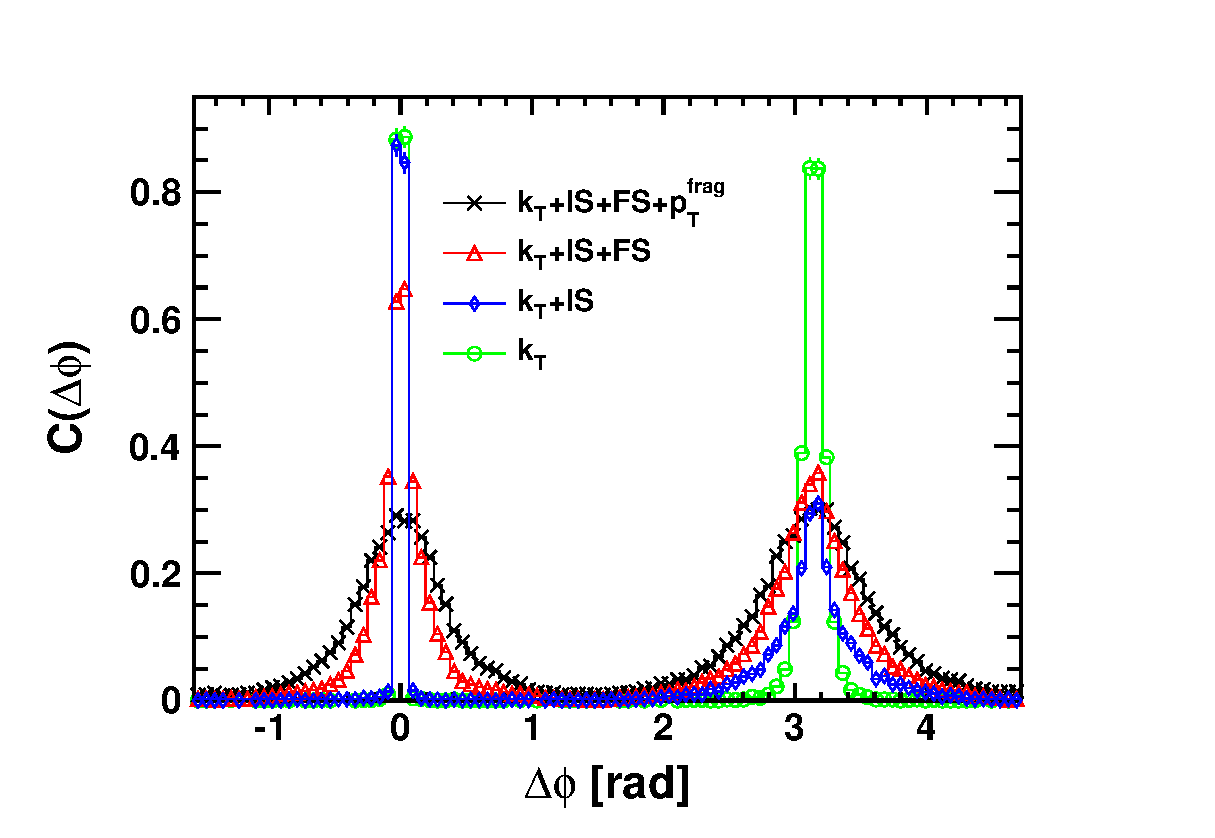
\includegraphics[width=0.7\textwidth]
{plots/chpt6/deltaPhi_20x100_Q2_1_y_0.7_Effects_decay.eps}
\end{center} 
%\captionsetup{width=0.9\textwidth}
\caption[effects in Monte Carlo on azimuthal diahdron correlation]
{
Comparison of dihadron correlation due to different physical inputs, such as 
intrinsic $k_T$, initial state parton shower (IS), final state parton shower plus 
resonance decay (FS) and $p_T$ broadening in fragmentation processes.
The \ep\ data are for charged hadrons with a beam energy of 20 GeV $\times$ 100 GeV 
with $1.0 \, \mathrm{GeV}^{2}  < Q^{2} < 1.5 \, \textrm{GeV}^2, 0.65 < y < 0.75, p_{T}^{trig} > 2 \,
\mathrm{GeV/}c, 1 \, \mathrm{GeV/}c < p_{T}^{assoc} < p_{T}^{trig}, 0.2 <
z_{h}^{trig}, z_{h}^{assoc} < 0.4$. 
}
\label{fig:dihadron_effects}
\end{figure}

\begin{figure}
\begin{center}
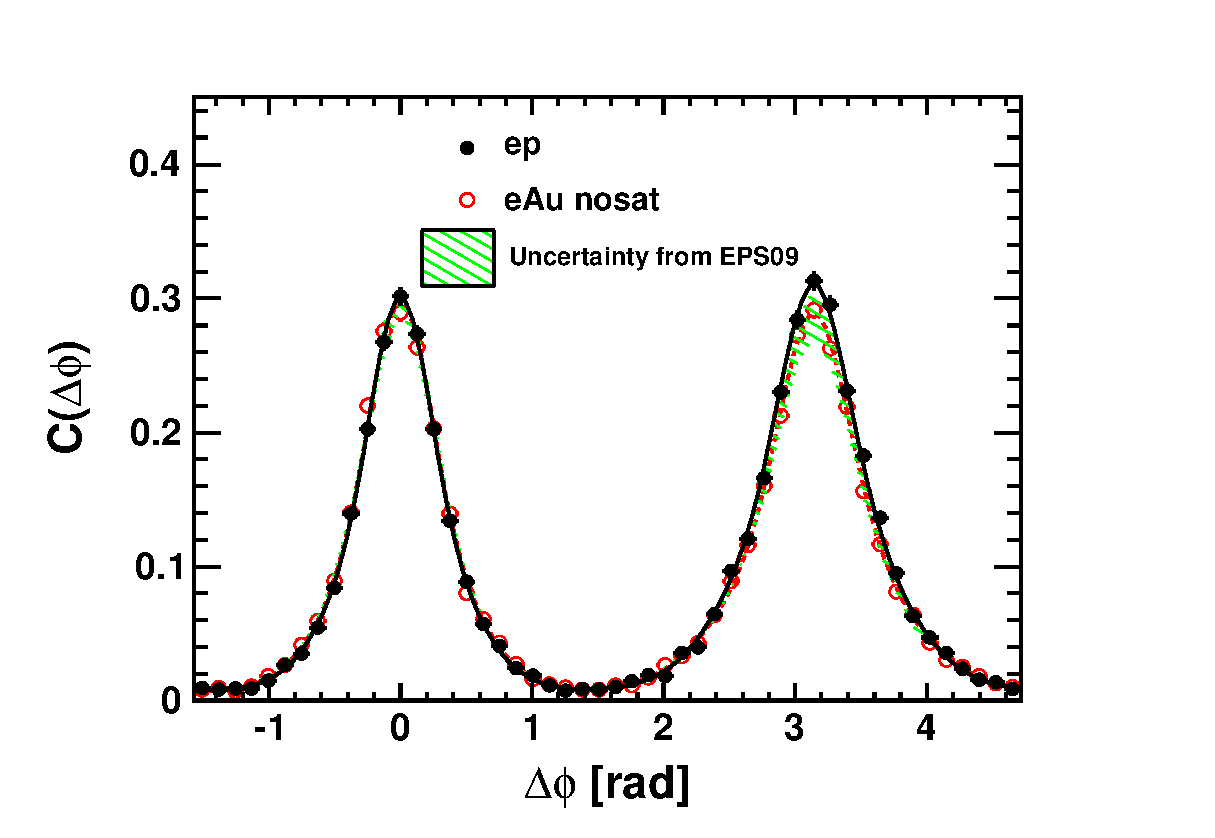
\includegraphics[width=0.7\textwidth]
{plots/chpt6/20x100_epAndeAu_Q2_1_y_0.7_uncertainty_EPS09_withfit.eps} 
\end{center} 
\caption[Monte Carlo result of diahdron correlation]{Simulated data points for particle correlations
for charged hadrons in \ep\ and \eAu\ collisions with beam energies of 20 GeV $\times$ 100
GeV and $1.0 \, \mathrm{GeV}^{2}  < Q^{2} < 1.5 \, \mathrm{GeV}^{2} , 0.65 < y < 0.75, p_{T}^{trig} > 2 \, \mathrm{GeV/}c, 1
\, \mathrm{GeV/}c < p_{T}^{assoc} < p_{T}^{trig}, 0.25 < z_{h}^{trig}, z_{h}^{assoc} <
0.35$. Lines are the fit for \ep\ or \eA\ points. The shaded band shows the uncertainty due to the EPS09 nuclear PDFs.
\label{fig:dihadron_base}}
\end{figure}

For our model of \eA\ implemented in PYTHIA, the effects due to energy loss
in the cold nuclear medium are expected to be weak, because fast moving partons are likely to
fragment outside the nucleus in the considered kinematic regions. Considering
that the nuclear PDF also has little impact on the $p_{T}$ imbalance of dijets,
it comes as no surprise to see very little change from \ep\ to \eA\ in the
simulation, as shown in Fig.~\ref{fig:dihadron_base}.
\begingroup
\begin{table} 
\centering 
\caption[table for effects on azimuthal correlation function]{Relative 
Root Mean Square (RMS) for the $\Delta\phi$ distribution from \ep\ collisions including
different effects influencing the width of the near and away side peak compared
to the baseline RMS with all the effects included (bottom row).}
\label{tab:azimuRMS} 
\begin{tabular}{ l  c  c  } \hline \hline
		& Near-side $\Delta\phi$ RMS & Away-side $\Delta\phi$ RMS \\ \hline
\kt		  	&  0.21  &  0.25   \\  
\kt+ IS     &  0.30  &  0.72   \\  
\kt+ IS + FS    & 0.65  &  0.81   \\  
\kt+ IS + FS + $p_T^{\textrm{frag}}$    &  1.00  & 1.00   \\ \hline \hline
\end{tabular} 
\end{table}
\endgroup
Table~\ref{tab:azimuRMS} is a reference for different effects on the relative root mean
square (RMS) deviation of the near/away side azimuthal correlation function,
from which we can clearly draw the conclusion that initial-state parton showers
dominate the away-side peak of the correlation function, while the near-side peak 
is mainly controlled by final-state effects such as final-state parton showers, 
fragmentation \pt and possible resonance decays in the fragmentaion.



\section{Analysis method}

In PYTHIA, depending on the wave function components for the incoming virtual
photon, various subprocesses are divided into three major classes: the direct
processes, the VMD processes and the anomalous processes~\cite{Friberg:2000ra},
as illustrated in Fig.~\ref{fig:PYTHIAFeyn}. The direct photon interacts as a
point-like particle with the partons of the nucleon, while the VMD and anomalous
components interact through their hadronic structure. The VMD component is
characterized by non-perturbative fluctuations of the photon into a $q\bar{q}$
pair existing long enough to evolve into a hadronic state before the subsequent
interaction with the nucleon ~\cite{Bauer:1977iq}. This process can be described
in the VMD model, where the hadronic state is treated as a vector meson (e.g.
$\rho^0$, $\omega$, $\phi$ ) with the same quantum numbers as the photon. These
VMD states can undergo all the soft/hard interactions with the nucleon allowed
in hadronic physics. The large-scale, perturbatively fluctuated photons can be
added as the anomalous photon part in a Generalized VMD (GVMD) model. Same pQCD
$2\rightarrow2$ process can be developed over the VMD or anomalous state of the
virtual photons on the target nucleon, with the difference that parameterized
photon PDFs are used for anomalous photons whereas for the hard VMD components
those vector meson PDFs are involved. Hard VMD and anomalous process are usually
referred to as ``resolved'' process. Resolved photon processes play a significant
part in the production of hard high-$p_{T}$ processes at $Q^{2}\approx0$. The
following hard subprocesses are grouped in the resolved processes category:
$qq\rightarrow qq, \, q\bar q \rightarrow q \bar q, \, q\bar q\rightarrow gg, \,
qg\rightarrow qg, \, gg\rightarrow q\bar q, gg\rightarrow gg$. In the
high-$Q^{2}$ region, direct processes become dominant, Fig.~\ref{fig:DISgraph}
shows the major subprocesses in that category: LO DIS, Photon-Gluon Fusion (PGF)
and QCD Compton (QCDC). As the PGF process is directly sensitive to the gluon
distribution, it is extremely important for DIS dijet productions. 


\begin{table} 
\centering
\begin{tabular} {|c|c|c|c|c|}
\hline
Subprocess			& \#&	Class	&	Description		&	group					 \\
\hline
$VN \rightarrow VN$	& 91& background& elastic VMD		& \multirow{5}{*}{Soft VMD}  \\
$VN \rightarrow VX$	& 92& background& single-diff VMD	& 							  \\
$VN \rightarrow XN$	& 93& background& single-diff VMD	&							  \\
$VN \rightarrow	XX$	& 94& background& double-diff VMD	&							  \\
$VN \rightarrow X$	& 95& background& soft non-diff VMD	&							  \\
\hline
$qq \rightarrow qq$	& 11& quark channel& \multirow{4}{*}{QCD $2\rightarrow 2$(q)} & \multirow{7}{*}{Resolved} \\
$q\bar{q} \rightarrow q\bar{q}$	& 12& quark channel&		&	\\
$q\bar{q} \rightarrow gg$	& 13& quark channel&			&	\\
$gq \rightarrow gq$	& 28& quark channel&					&	\\

$qg \rightarrow qg$	& 28& gluon channel	& \multirow{3}{*}{QCD $2\rightarrow 2$(g)} &	\\
$gg \rightarrow q\bar{q}$ & 53& gluon channel&				&	\\
$gg \rightarrow gg$	& 68& gluon channel	&					&	\\
\hline
$\gamma^{*}q \rightarrow q$	& 99& background& LO DIS	&	\multirow{5}{*}{Direct}	\\
$\gamma^{*}_{T}q \rightarrow qg$ & 131& quark channel& (transverse) QCDC	&	\\
$\gamma^{*}_{L}q \rightarrow qg$ & 132& quark channel& (longitudinal) QCDC	&	\\
$\gamma^{*}_{T}g \rightarrow q\bar{q}$ & 135& gluon channel& (transverse) PGF	&	\\
$\gamma^{*}_{L}g \rightarrow q\bar{q}$ & 136& gluon channel& (longitudinal) PGF	&	\\
\hline
\end{tabular}
\caption[subprocess list in PYTHIA]{Accessible subprocess list used in PYTHIA. $V$ represents vector meson, $\gamma^{*}_{L/T}$ denotes a longitudinal/transverse virtual photon. Respective process id,  classification, and name used in this work are presented in this table.}\label{tab:processList}
\end{table}


The full accessible process list and its classification has been summarized in
Tab.~\ref{tab:processList}. Corresponding subprocess id in PYTHIA can also be found in this table. The soft process ($91-95$) and LODIS (99)
process, the transverse momentum transfer is very small. They don't contribute
to the high-$p_{T}$ correlated particle pairs. At small $x$, gluon behaviors
dominate in the dihadron correlations studies. Accordingly, we are expecting to
see the gluon channels sensitive to the gluon saturation effect. Considering the
saturation physics introduces a suppression to correlation function from \ep\ to
\eA\ as suggested in Eq.~(\ref{fig:dihadron_theory_sud}), the final conditional
yield can be expressed as a superposition from different processes:
\begin{equation} 
C(\Delta\phi)=\Sigma_{i}w_{i}w^{s}_{i}C(\Delta\phi)_{i},
\label{eqn:subprocess} 
\end{equation}
with $w_{i}$ being the statistical weight of every subprocess $i$ involved in
the measurement and $w^{s}_{i}$ is the suppression factor for the subprocess $i$
from \ep\ to \eA\ due to saturation. For the quark channels unaffected by saturation $w^{s}_{i}=1$,
while for the gluon channels, suppression of $C(\Delta\phi)$ at away-side is
expected with $w^{s}_{i}<1$.

\begin{figure*} 
\begin{center} 
\subfigure[]{ 
\centering
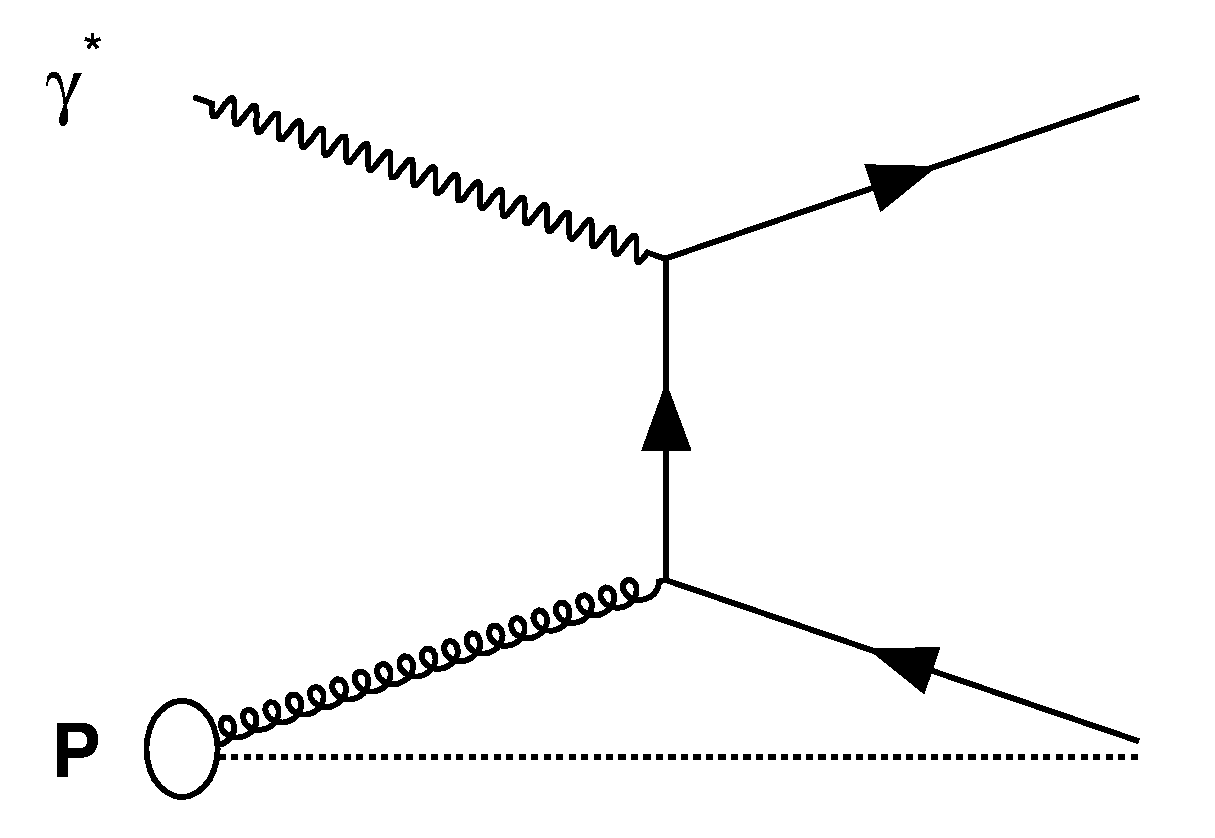
\includegraphics[width=0.25\textwidth]{plots/chpt6/feynman/Direct.eps} \label{fig:Direct} 
}
\quad 
\subfigure[]{ 
\centering
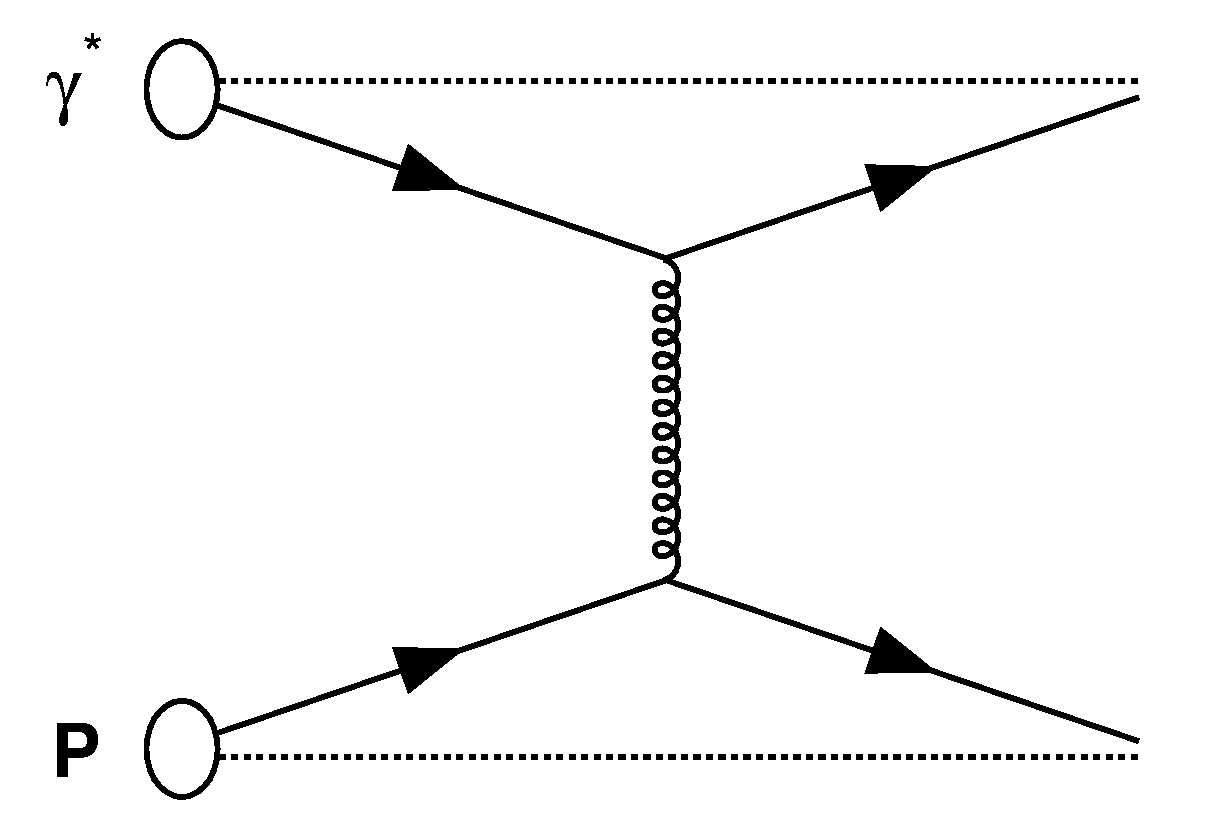
\includegraphics[width=0.25\textwidth]{plots/chpt6/feynman/VMD.eps} \label{fig:VMD} 
} 
\quad
\subfigure[]{ 
\centering
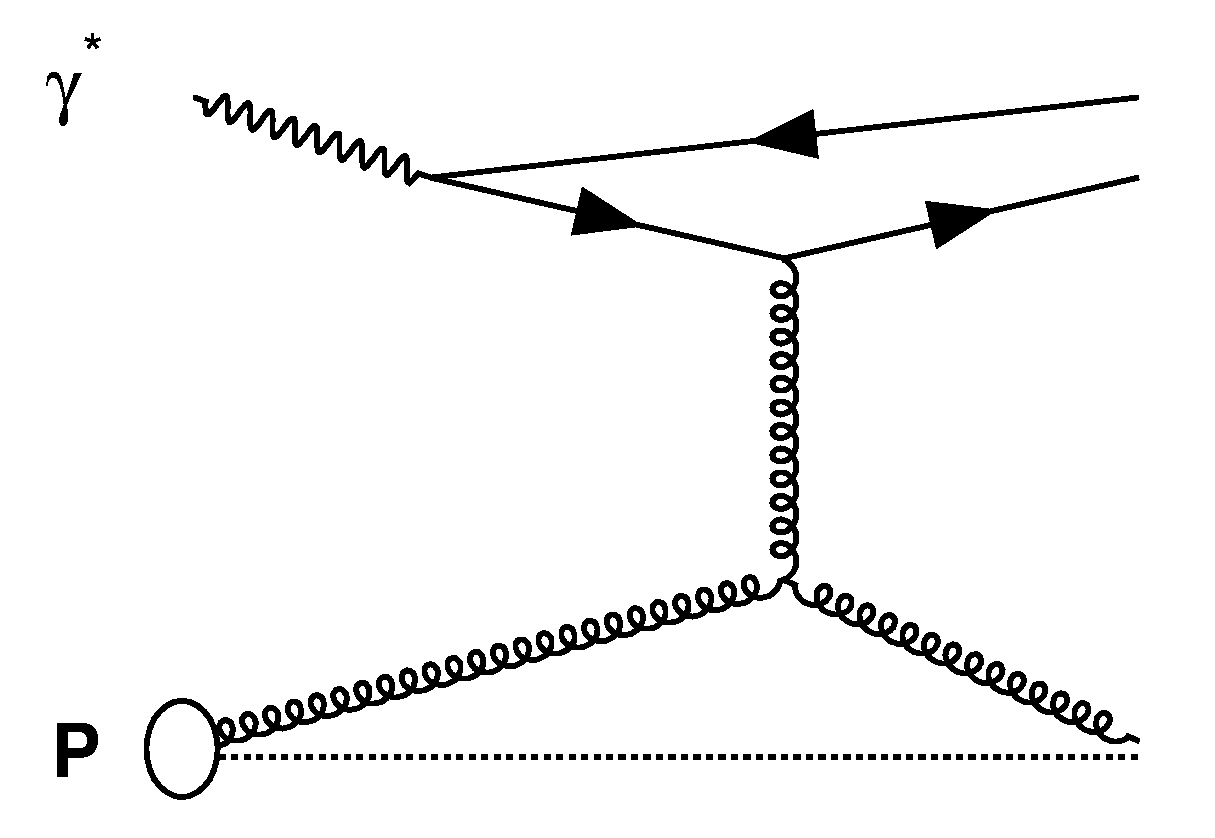
\includegraphics[width=0.25\textwidth]{plots/chpt6/feynman/Anomalous.eps} \label{fig:Anomalous} 
}
\caption[PYTIHIA subprocess categories]{Feynman diagrams for different
PYTHIA subprocesses contributing to the hard interaction: (a) direct, (b) VMD,
(c) anomalous. The dotted lines indicate the presence of a spectator. Bubbles
stand for a hadron or hadronic structure.}
\label{fig:PYTHIAFeyn} 
\end{center} 
\end{figure*}


As the saturation physics discussed above is mainly about the gluon dynamics, in
order to be able to consistently compare with the theoretical dihadron cross
section in Sec.~\ref{sec:dihadrontheory}, we need to include gluon dijet channels from
PGF and gluon-initiated resolved process in the comparison. However, as the
measured observable in the real experiment is a mixture of different process, as
illustrated in Eq.~(\ref{eqn:subprocess}), we have to know how significant the
signal from gluon saturation manifests itself in a mixed event sample. From the
saturation-based predictions, a sizeable suppression of the away-side peak from \ep\
to \eA\ is expected.

In the meanwhile, it is crucial to point out that parton showers suppress the
away-side peak of the dihadron correlation function just like saturation does.
However, currently it is still unclear how the parton shower effect is modified
in the nuclear medium, without which it is hard to draw any definite conclusions
about the saturation effects, as parton showers and saturation effects are always
entangled. Nevertheless, thanks to the large kinematic coverage of eRHIC, one
can explore the nuclear dependence of parton showers outside the saturation
region by measuring dihadron correlations for different nuclei in the high
$Q^2$ regime. This kinematic regime has a significant phase space for parton
showers for this observable. More importantly, the measurement of dihadron
correlations gives the opportunity to use the near-side peak of the correlation
function as a reference to study the nuclear medium effects on parton showers as
the saturation effects only manifest themselves in the away-side peak, as shown
in Fig.~\ref{fig:dihadron_effects}.

In the saturation formalism, the parton shower contribution is effectively cast
into the Sudakov factor for the DIS dijet process at small $x$. To illustrate this
point, Fig.~\ref{fig:epCompareWithSud} shows the correlation function simulated
with and without parton showers, compared to the corresponding theoretical
predictions with and without Sudakov effects. The filled circles represent the PYTHIA
simulation for \ep\ without parton showers, and they agree very well with the solid
line from the theoretical prediction including saturation effects, but excluding
Sudakov effects. The comparison (empty circles and dashed line) between simulated PYTHIA \ep\
data including parton showers and the theoretical predictions with
saturation plus Sudakov effects is also good, especially considering the model
uncertainties. Thus, the agreement in \ep\ collisions enables one to estimate the
nuclear medium effects on parton showers in the theoretical predictions for
saturation including Sudakov effects.

Since the saturation effect decouples from hadronization, it does not
depend on which specific particle type being detected. Although the theoretical
prediction is made for $\pi^{0}$, the suppression factor from \ep\ to \eA\
still holds for other different final state particles. In the next section, the
significance for the suppression of gluon saturation will be shown for the
charged hadrons $C(\Delta\phi)$ observable with limited statistics and
expected background estimation.
\begin{figure} 
\begin{center}
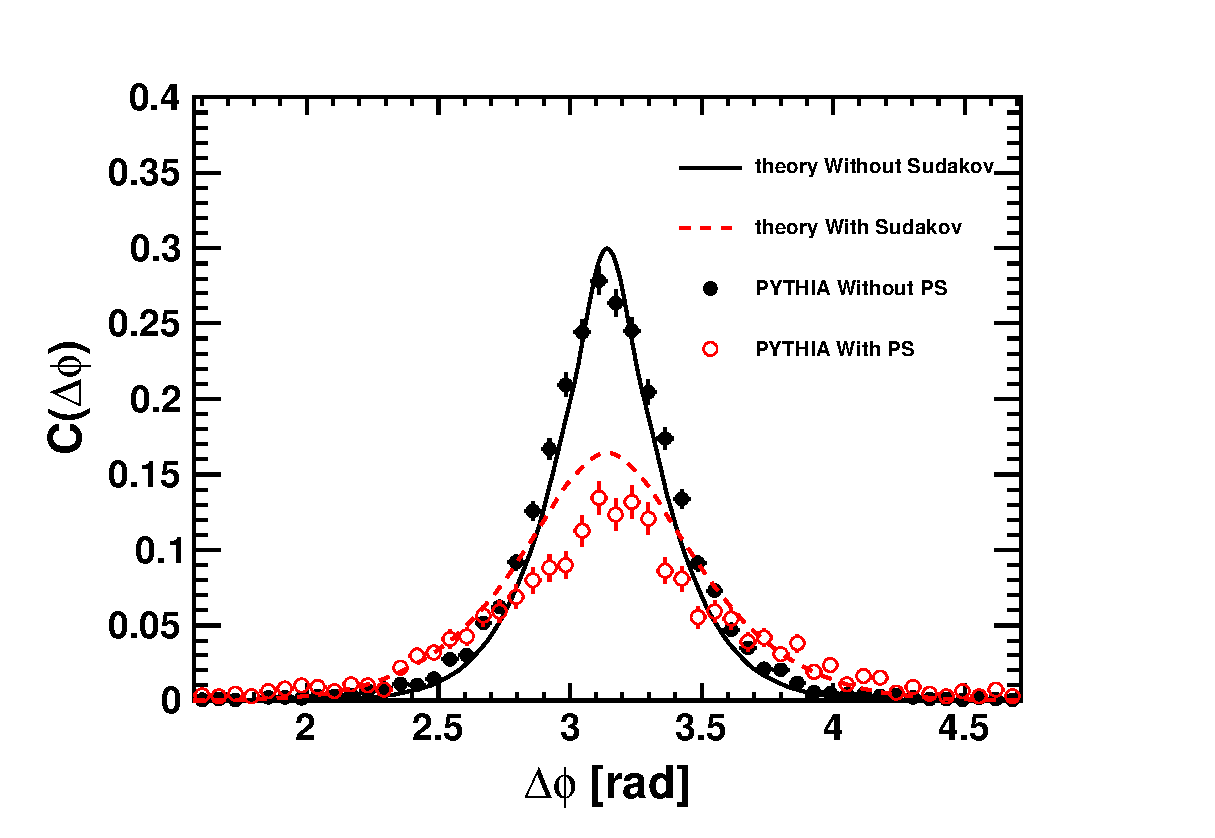
\includegraphics[width=0.7\textwidth]{plots/chpt6/ep_10x100_Q2_1_y_0.7_theory_MC_compare_as_0.35.eps} 
\end{center} 
\caption[comparison of ep from PYTHIA and theory with Sudakov]
{\pion $\Delta\phi$ correlation comparing PYTHIA and theoretical saturation calculations
for \ep\ 10 GeV $\times$ 100 GeV for events from PGF and resolved gluon channel subprocesses
 at $1.0 \, \mathrm{GeV}^{2} < Q^{2} < 2.0 \, \mathrm{GeV}^{2}$, \, $0.65 < y < 0.75, \, p_{T}^{trig} > 2 \,
\mathrm{GeV/}c, 1 \, \mathrm{GeV/}c < p_{T}^{assoc} < p_{T}^{trig}, \,0.25 <
z_{h}^{trig}, z_{h}^{assoc} < 0.35$. The solid and dashed curves show theoretical predictions including 
saturation effects for \ep\ without and with Sudakov factor, respectively. 
The filled and empty circles illustrate PYTHIA simulations for \ep\ without and with parton showers. }
\label{fig:epCompareWithSud} 
\end{figure}


\section{Kinematics reconstruction and event selection}
The kinematic variables of an event are very important for the physics analysis.
Experimentally, the kinematic variables can be reconstructed in several ways.
One of the common ways is to reconstruct from the scattered leptons. In this
method, the scattered lepton must be identified. At eRHIC, for intermediate
$Q^{2}$ values, it is the scattered electron to be found. With the energy
($E^{'}_{e}$), scattering angle ($\theta_{e}$) of this scattered electron and
the incoming electron beam energy ($E_{e}$), one can extract all the kinematic
information for that event. Considering that these variables are actually
correlated, only two variables need to be reconstructed and all the others can
be calculated from these two. Practically, we usually reconstruct the kinematic
variables $Q^{2}$ and $y$ as follows:
\begin{align}
Q^{2}=2E_{e}E^{'}_{e}(1-cos\theta_{e}), \\ \nonumber
y=1-\frac{E^{'}_{e}}{E_{e}}cos^{2}(\theta_{e}/2).
\label{eqn:electr_method}
\end{align}
All the other kinematics variables can be obtained based on these two and
the knowledge of the beam energy. 

When $Q^{2}$ is very large  (electroweak interaction happens), the scattered
lepton will be a neutrino that can not be captured by our detector system. A
different method, the Jacquet-Blondel (JB) method must be applied. This method
reconstructs event kinematics from all the hadronic final state particles.
\begin{align}
(E-p_{z})_{h} = \sum_{h}(E_{h}-p_{z}^{h}), \\ \nonumber
p_{T,h}^{2} = (\sum_{h}p_{x,h})^{2}+(\sum_{h}p_{y,h})^{2}, \\ \nonumber
y_{JB}=\frac{(E-p_{z})_{h}}{2E_{e}}, \\ \nonumber
Q_{JB}^{2}=\frac{p_{T,h}^{2}}{1-y_{JB}}.
\end{align}

Other methods for kinematics reconstruction can be found in
Ref.~\cite{Blumlein:2012bf}. In the following studies, we will use electron
method to reconstruct the event kinematics. 


%
%\section{Electron-Ion Collider and Simulations}\label{sec:MC}
%
%\subsection{The Electron-Ion Collider and its Detector}
%
%Two independent designs for an EIC are being developed in the United States:
%eRHIC, at Brookhaven National Laboratory (BNL); and MEIC/ELIC at Thomas
%Jefferson National Laboratory (JLab). The following studies will focus on the
%eRHIC version of an EIC and the new model detector at eRHIC. The eRHIC design at
%BNL reuses the available infrastructure and facilities of RHIC's high-energy
%polarized proton/ion beam. A new electron beam, based on Energy Recovery LINAC
%(ERL) technology, is to be built inside the current RHIC tunnel. At eRHIC, the
%collision luminosity is expected to be in the order of $10^{33-34}
%\textrm{cm}^{-2}\textrm{s}^{-1}$. The full range of proton/ion beam energies will be accessible
%from the beginning of operations, while the electron beam energy will start with
%$10-15$ GeV and later be increased to $20$ GeV.
%
%The tracking system of the baseline eRHIC detector will consist of a TPC, GEM
%and silicon detectors spanning a range of $-4<\eta<4$ in pseudorapidity. The
%end-cap and barrel region on the detector will be equipped with electromagnetic
%calorimeters covering $-4.5<\eta<4.5$. Hadronic calorimeter will be used mostly
%for jet physics at full energy in the forward (hadron beam going direction) and
%backward (electron beam going direction) rapidities spanning $2<|\eta|<4.5$.
%Projected momentum and energy resolutions of these devices are better than a few
%percent, which extends the capability of this detector to a large variety of
%physics topics.



The present study is based on the planned lepton and nucleon beam energy of 10
GeV $\times$ 100 GeV and 20 GeV $\times$ 100 GeV. The kinematics are constrained
to the main region of interest for dihadron correlation studies,
$1\, \textrm{GeV}^{2}<Q^{2}<20 \, \textrm{GeV}^{2}$ and
$0.01<y<0.95$. 

\begin{figure} 
\begin{center}
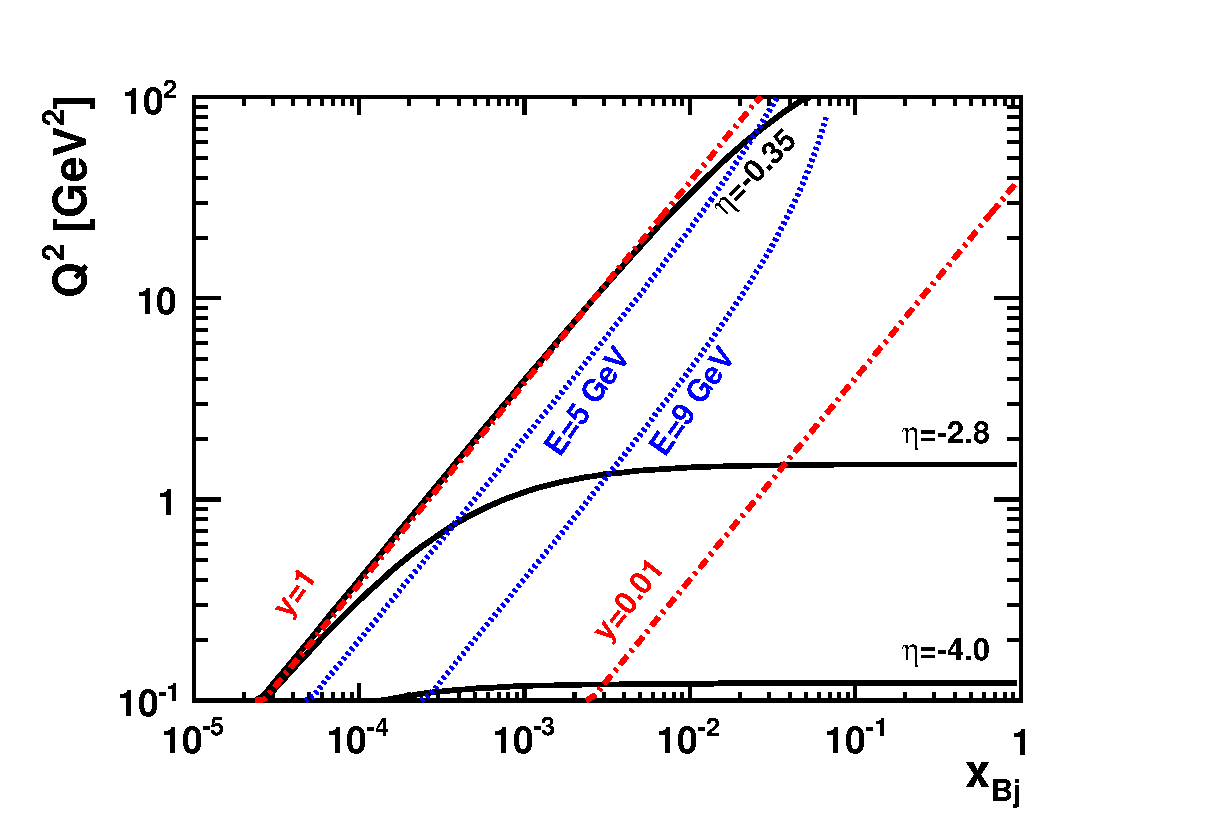
\includegraphics[width=0.7\textwidth]
{plots/chpt6/Q2vX_eta_E.eps}
\end{center} 
\caption[Contours of fixed scattered electron kinematics]{Kinematics distribution for \ep\ 10 GeV $\times$100 GeV with 
scattered electron at fixed pseudorapidity (shown in black line) or energy (blue dotted line). The kinematic coverage
of $y=0.95$ and $y=0.01$ has been marked out the red dashed line.  
.}
\label{fig:scattered_electron}
\end{figure}

As observed in Fig.~\ref{fig:scattered_electron}, in the kinematics region we are interested in,
backward electromagnetic calorimetry and the tracking system will be utilized for
reconstruction of the event kinematics (based on the electron method). As shown in
Fig.~\ref{fig:Q2VsxBj}, abundant high-\pt particles will be generated in the
specified kinematic region to make correlated hadron pairs even with a limited
luminosity of 1 fb$^{-1}$. Among those generated high-\pt particles,
Fig.~\ref{fig:PtSpectrum} suggests that gluon dijet processes dominate in the
production of particles with a transverse momentum greater than 2 GeV/$c$ and
charged pions are the major component for the final state particles.


\begin{figure*} 
\begin{center}
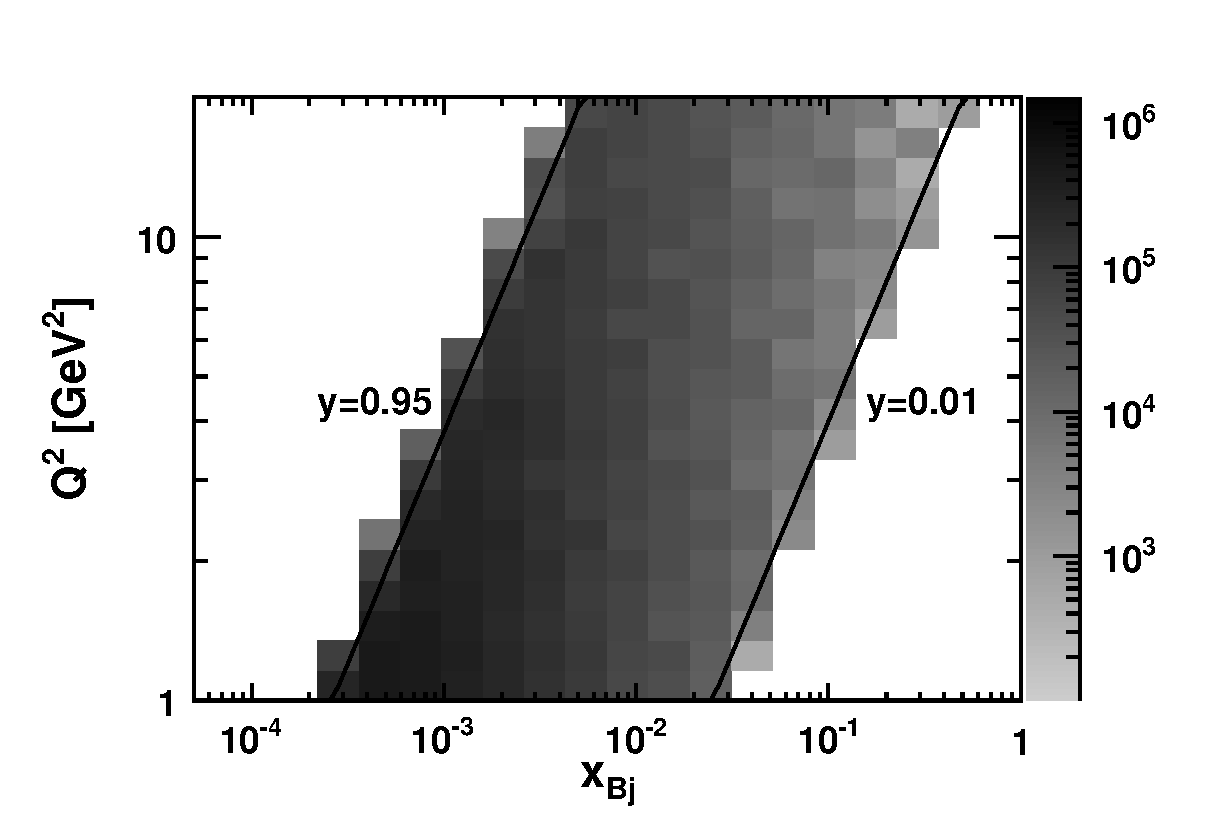
\includegraphics[width=0.45\textwidth]
{plots/chpt6/q2vx_paircount_10x100_1fb-1.eps}
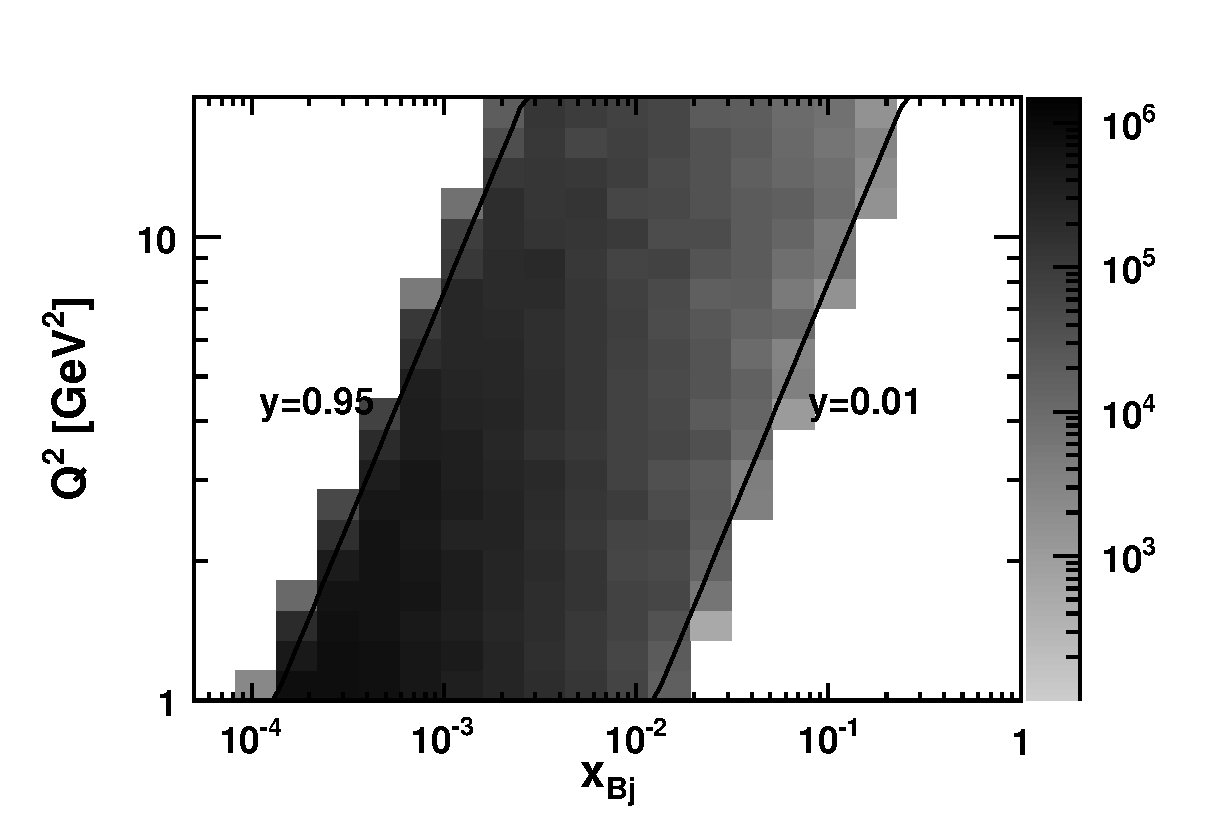
\includegraphics[width=0.45\textwidth]
{plots/chpt6/q2vx_paircount_20x100_1fb-1.eps}
\end{center} 
\caption[Statistics in allowed kinematics region]{Expected yields of charged
particle pairs at transverse momentum $p_{T}>1$ GeV/$c$ in bins of 
($Q^{2}$, $x_{Bj}$) for an integrated luminosity of 1 fb$^{-1}$ for 
\ep\ 10 GeV $\times$100 GeV (Left) and 20 GeV $\times$100 GeV (Right) in the kinematic
range of $1\, \textrm{GeV}^{2}<Q^{2}<20 \, \textrm{GeV}^{2}$, and $0.01<y<0.95$.}
\label{fig:Q2VsxBj}
\end{figure*}

\begin{figure*} 
\begin{center} 
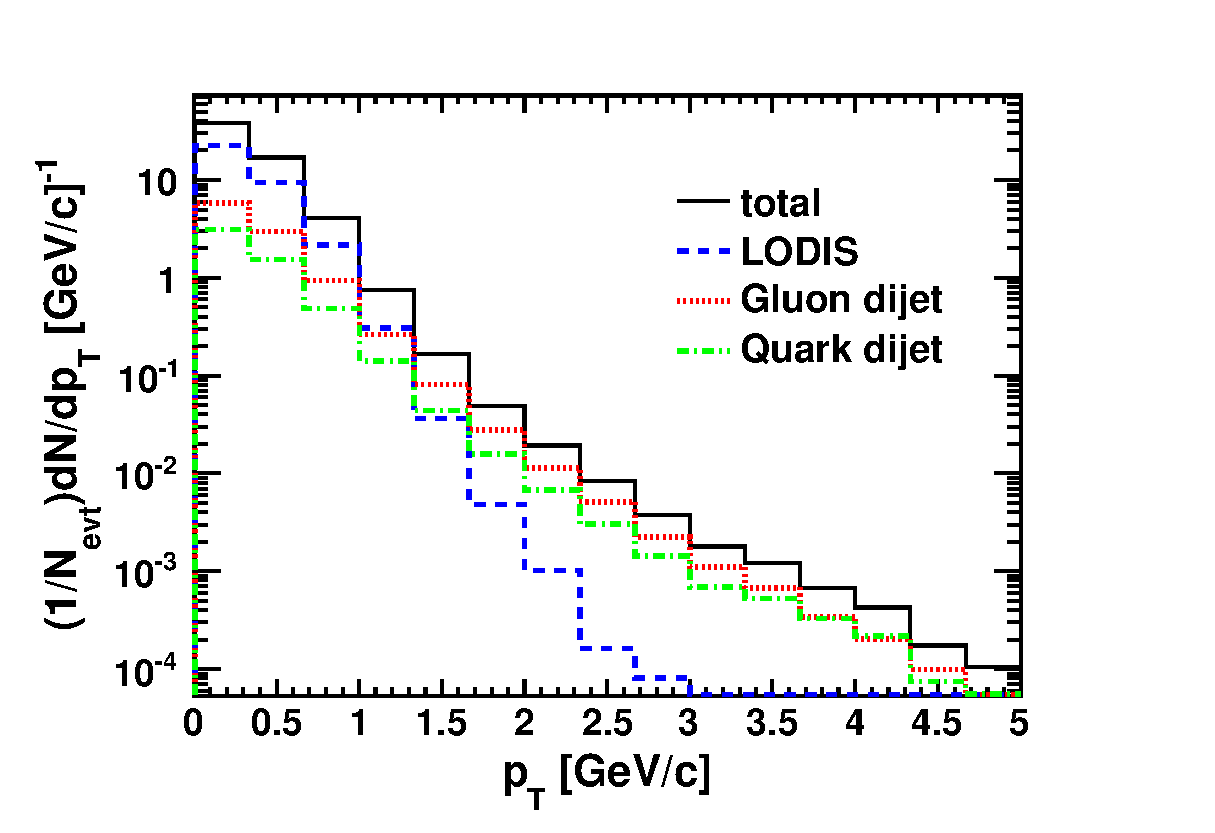
\includegraphics[width=0.45\textwidth]
{plots/chpt6/ep_10x100_Q2_1_20_y_0.01_0.95_process_ptSpectrum.eps}
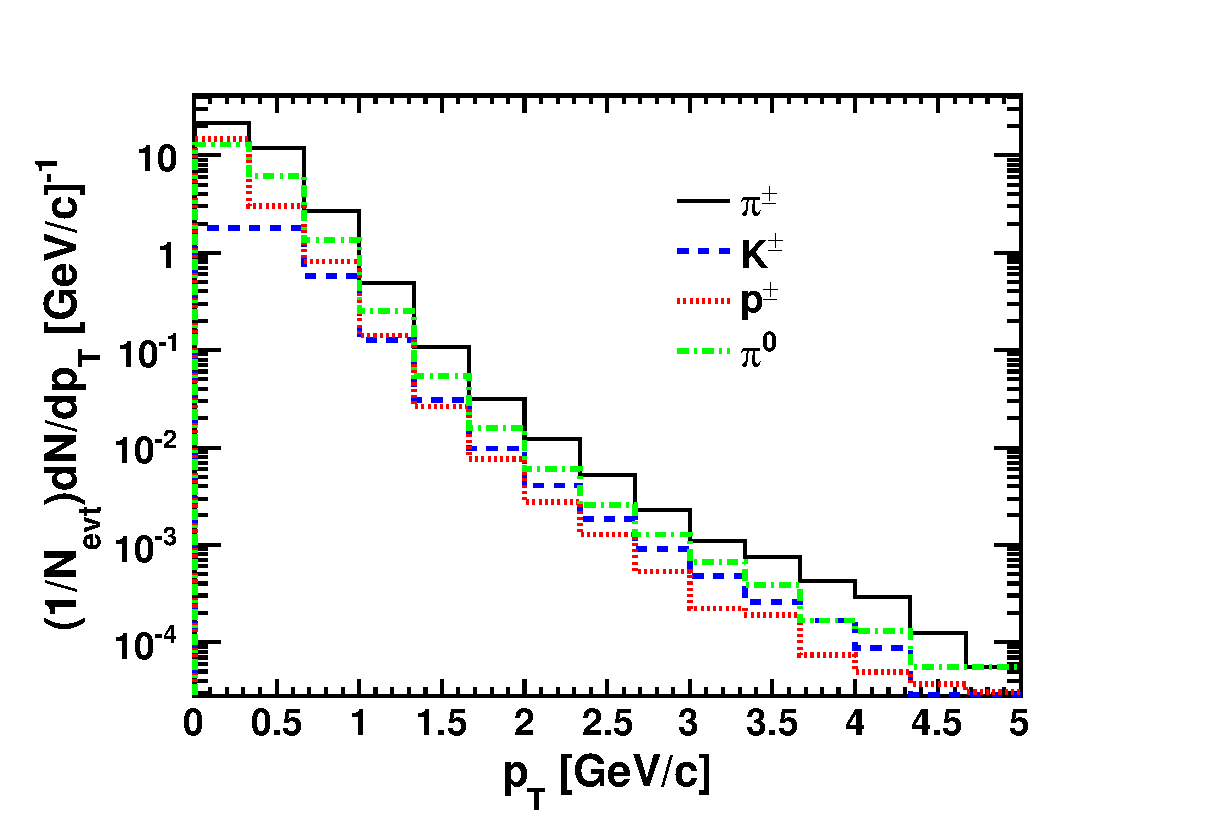
\includegraphics[width=0.45\textwidth]
{plots/chpt6/ep_10x100_Q2_1_20_y_0.01_0.95_PID_ptSpectrum.eps}
\end{center} 
\caption[Process or PID dependent pt distribution]
{Particle $p_{T}$ distributions for \ep\ 10 GeV $\times$ 100 GeV collisions with
$1 \, \mathrm{GeV}^{2}  < Q^{2} < 20 \, \mathrm{GeV^{2}}, 0.01 < y < 0.95$. Left: charged particle production from LO DIS, gluon dijets
(PGF and resolved gluon channel) and quark dijets (QCDC and resolved quark channel).
Right: $\pi^{\pm}, K^{\pm}, p^{\pm}$ and $\pi^{0}$ production for all processes.}
\label{fig:PtSpectrum}
\end{figure*}

The event selections are targeting to extract the most prospective kinematics
region sensitive to the physics message we are looking for and also validates
the requirement of our theoretical calculations. In order to guarantee the
validity of perturbative calculations and avoid the kinematic regime of
quasi-real photo-production, a cut of $Q^{2}>1 \, \mathrm{GeV}^{2}$ is generally
made. On the other hand, probing the saturation dynamics requires to probe the
dense region, which means that one needs to go to low $x$ and low-to-moderate
$Q^{2}$ in the pursuit of saturation effects at a certain center of mass energy.
A cut in transverse momentum of the charged hadron pairs is usually performed to
pick particles from hard interactions. A cut on $z_{h}$ is also imposed to
reject particles from the target remnants. As indicated in Fig.~\ref{fig:trig_kinematic},
PGF process is the most significant process for the generation of high-$p_{T}$ particles. 
Choice on the cut of trigger particle should not be too large $p_{T}$ and $z$ is
better to be intermediate. Thus, a typical cut to select dihadron pairs from hard parton
scatterings is: $p_{T}^{trig}>2$ GeV/$c$, $1 \, \mathrm{GeV/}c
<p_{T}^{assoc}<p_{T}^{trig}, 0.2<z_{h}^{trig},z_{h}^{assoc}<0.4$.

The hadron pair selection iteration loops as: first, test if the current event is in
our selected $Q^{2}-x_{Bj}$ bin; second, choose the particle with the highest
$p_{T}$ in that event as the trigger particle which passes the trigger particle cut criteria;
after that, the particles which satisfy the associate cut criteria will be identified
as the associate. By pairing the trigger particle with every associate particle, we can
make the conditional yield $C(\Delta\phi)=\frac{N_{pair}(\Delta\phi)}{N_{trig}}$.


\begin{figure*} 
\begin{center} 
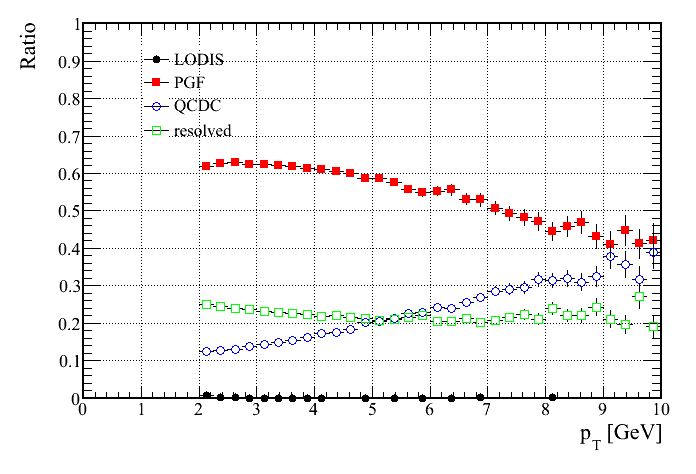
\includegraphics[width=0.45\textwidth]
{plots/chpt6/ep_20x100_y_0.7_Q2_4_trigPt_ratio.png}
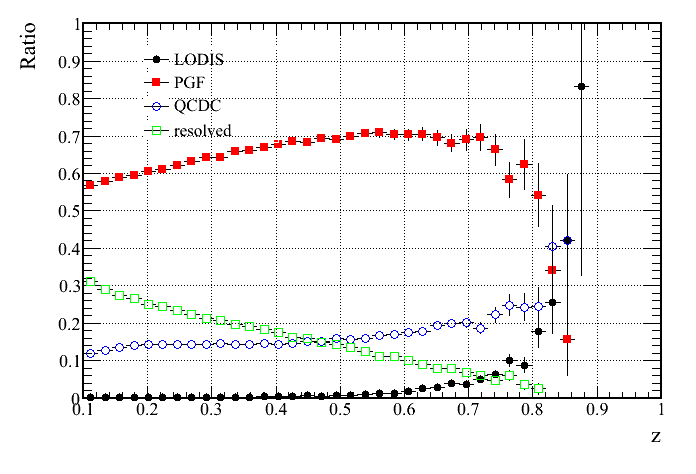
\includegraphics[width=0.45\textwidth]
{plots/chpt6/ep_20x100_y_0.7_Q2_4_trigZ_ratio.png}
\end{center} 
\caption[Process fraction depending on trigger particle kinematics]
{Event fraction depending on the leading particle (charge particle with highest $p_{T}$ in that event) transverse momentum and $z$
for the event at \ep\ 20 GeV $\times$ 100 GeV when leading particle $p_{T}>2\mathrm{GeV}/c, z>0.1$.}
\label{fig:trig_kinematic}
\end{figure*}


\section{Monte Carlo results and uncertainties} 
 To further explore the
transition behavior in and out of the saturation region, we use three $Q^{2}$ bins:
$1\, \textrm{GeV}^{2}<Q^{2}<2 \, \mathrm{GeV}^{2}$, $3\, \textrm{GeV}^{2}<Q^{2}<5 \,
\mathrm{GeV}^{2}$ and $9\, \textrm{GeV}^{2}<Q^{2}<20 \, \mathrm{GeV}^{2}$; and two $y$ bins:
$0.25<y<0.35$ and $0.6<y<0.8$. To study saturation physics using varying heavy
ion beams, we focus on the $1\, \textrm{GeV}^{2}<Q^{2}<2 \, \mathrm{GeV}^{2}$, $0.6<y<0.8$
bin, while the $9\, \textrm{GeV}^{2}<Q^{2}<20 \, \mathrm{GeV}^{2}$ or $0.25<y<0.35$ bins serve
as a reference for the behaviour without saturation effects. To pin down the
nuclear dependence of parton showers, we compare the correlation between \ep\
and \eA\ collisions for bins without saturation effects.
\begin{figure}
\begin{center}
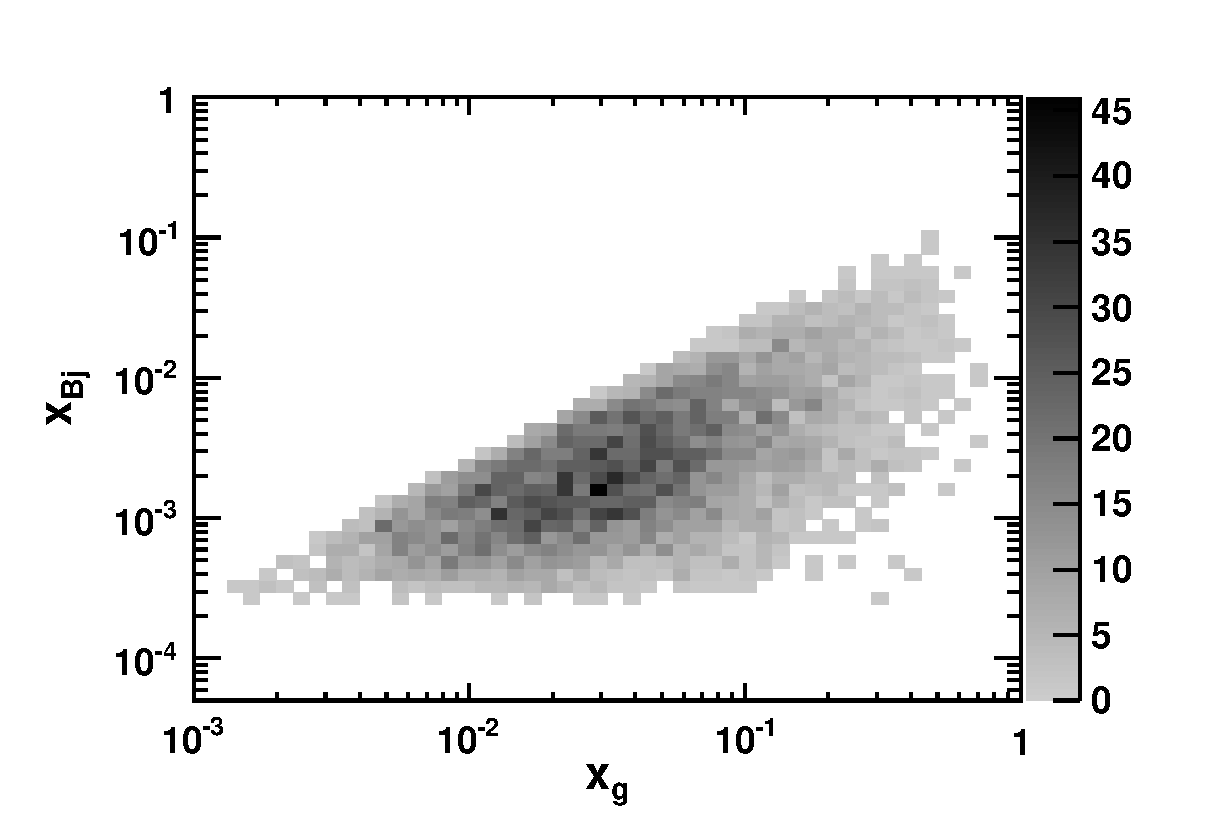
\includegraphics[width=0.7\textwidth]{plots/chpt6/xbjVsxg_highPtPairs_PGF_10x100.eps}
\end{center}
\caption[Correlation of $x_g$ and $x_{Bj}$]{The correlation of $x_{Bj}$ vs $x_{g}$ for the PGF process for \ep\ at 
10 GeV $\times$ 100 GeV with $0.01<y<0.95$, $1\, \textrm{GeV}^{2}<Q^{2}<20 \, \mathrm{GeV^{2}}$. A relatively 
broad correlation between these two variables is observed. }
\label{fig:xbjVsxg}
\end{figure}
Because the saturation scale $Q_{s}$ varies with the gluon momentum fraction
$x_{g}$, it is important to have access to $x_{g}$.
Fig.~\ref{fig:xbjVsxg} shows how, by utilizing $x_{Bj}$, one can
effectively constrain the underlying $x_{g}$ distribution. Although this is only
a broad correlation, it is demonstrated in Fig.~\ref{fig:xgCover} that
the typical $x_{g}$ at a given $x_{Bj}$ is constrained to a certain magnitude and can be used to
separate the saturation region from the non-saturated region.
\begin{figure*}
\begin{center}
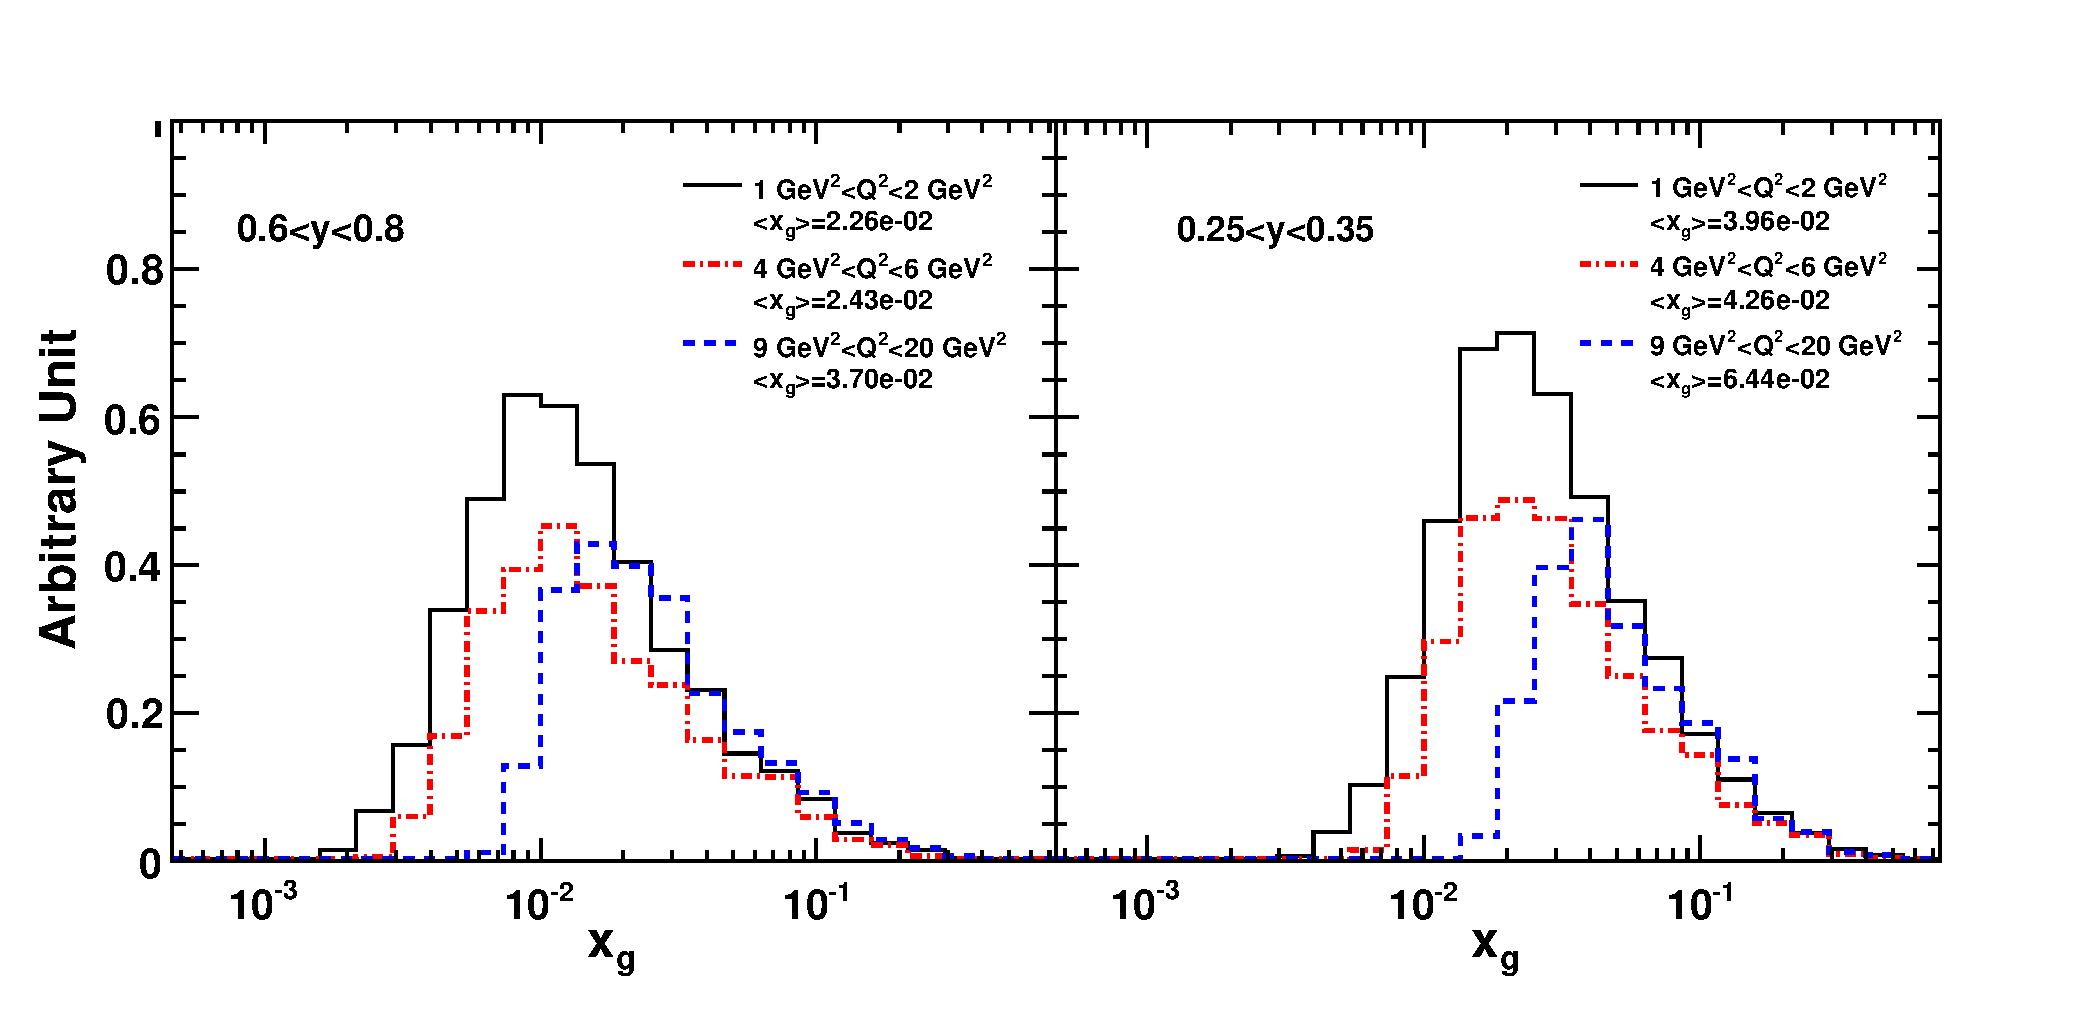
\includegraphics[width=1.0\textwidth]{plots/chpt6/ep_10x100_xg_distribution_multibins.eps} 
\end{center} 
\caption[$x_{g}$ coverage]{$x_{g}$ distributions in various kinematics bins
probed by the correlated hadron pairs in the PGF process for \ep\ 10 GeV
$\times$ 100 GeV. }
\label{fig:xgCover} 
\end{figure*}
Fig.~\ref{fig:pairEta} shows the $\eta$ distribution of the trigger
particle and the correlated particle in the aforementioned kinematic
bins at 10 GeV $\times$ 100 GeV and 20 GeV $\times$ 100 GeV. Clearly, with a
charged particle acceptance spanning $-4.5<\eta<4.5$, both trigger and
associate particles in our kinematics binning scheme can be fully accepted by
the detector.
\begin{figure*}
\begin{center}
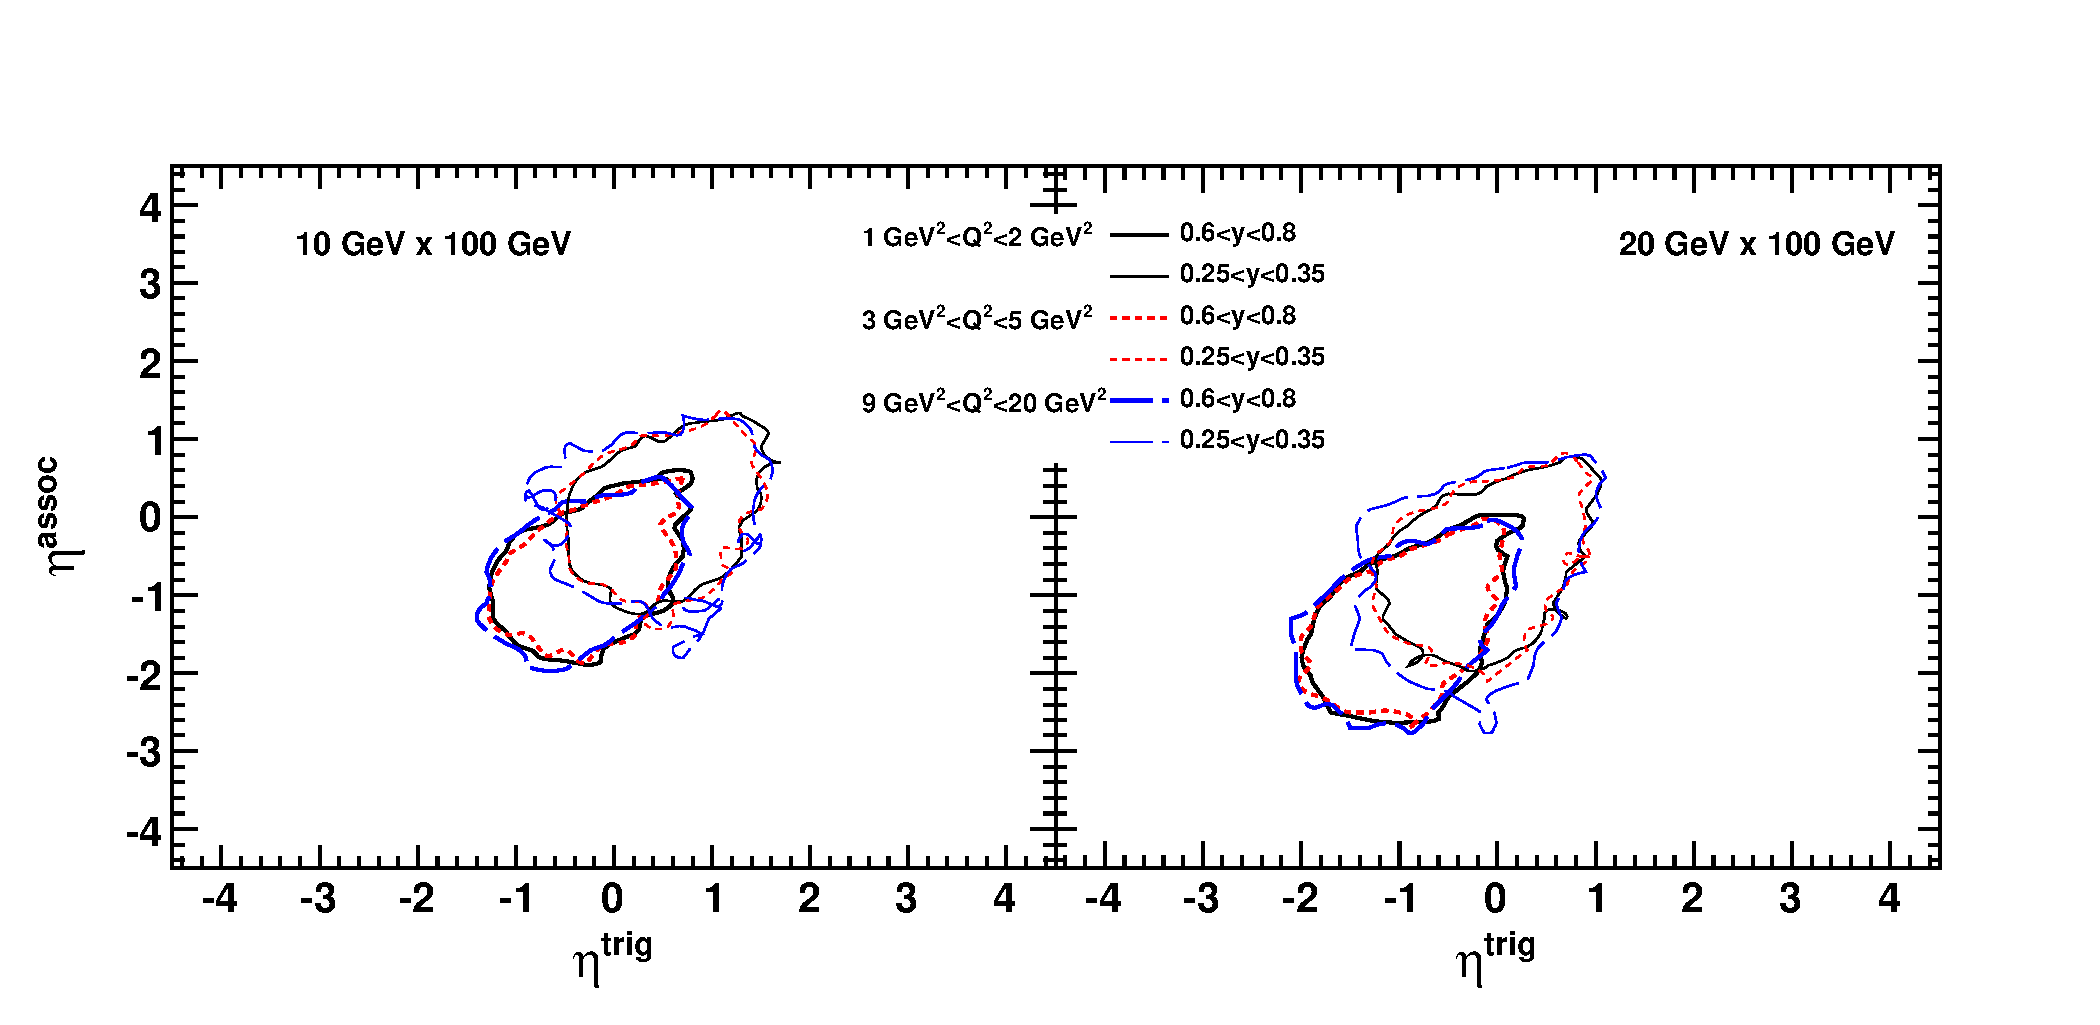
\includegraphics[width=1.0\textwidth]{plots/chpt6/ep_10And20x100_trig_2_asso_1_z_0.2_0.4_multiBin_etaCorre.eps}
\end{center} 
\caption[dihadron pair $\eta$ distribution]{The contours show the
$\eta$ regions covered by the correlated dihadron pairs: for 10 GeV $\times$ 100
GeV and 20 GeV $\times$ 100 GeV. Thick lines mark out the region for $0.6<y<0.8$
while thin lines for $0.25<y<0.35$.}
\label{fig:pairEta} 
\end{figure*}


\begin{figure}
\begin{center}
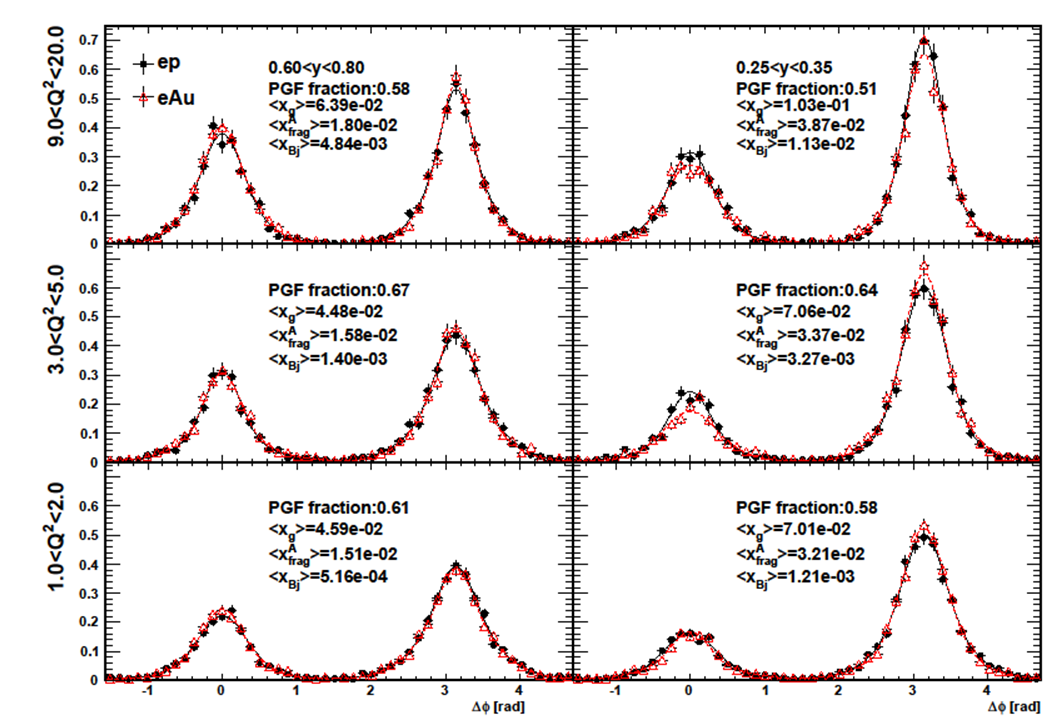
\includegraphics[width=1.0\textwidth]{plots/chpt6/10x100_multiBin_correlation.png}
\end{center} 
\caption[Dihadron correlation in multiple bins]{This panel shows dihadron correlation for \ep\ and \eAu\ 10 GeV $\times$ 100 GeV in multiple kinematics bins $1\, \textrm{GeV}^{2}<Q^{2}<2 \, \mathrm{GeV}^{2}$, $3\, \textrm{GeV}^{2}<Q^{2}<5 \,
\mathrm{GeV}^{2}$ and $9\, \textrm{GeV}^{2}<Q^{2}<20 \, \mathrm{GeV}^{2}$ $\otimes $
$0.25<y<0.35$ and $0.6<y<0.8$.}
\label{fig:dihadronMulti} 
\end{figure}

Fig.~\ref{fig:dihadronMulti} shows the conditional yield function in various
kinematics bins, from which we can read about the interplay of
underlying kinematics and the cut preference. The relative near-side away-side
peak yield changes with $y$ due to the selection of trigger $p_{T}$ cut. At
lower $y$, the center of mass energy at hard interaction is smaller. After taken
out a trigger particle, the near-side jet energy is not enough to produce
another particle fits into the associate, which aggregates most of the associate
particle at away-side peak. As to the evolution in $Q^{2}$, two factors play a
significant role. Higher $Q^{2}$ produces harder jet $p_{T}$ spectrum. Also
parton shower becomes stronger in high $Q^{2}$ enhancing the yield of particles.
However, it is still unknown how parton shower is going to be changed in the nuclear
medium. Here, we just assume that it is the same. But more systematic
studies can be done when the real data comes.


As shown in Fig.~\ref{fig:dihadron_theory_sud}, if we are in a kinematic regime
in $x$ and $Q^2$ where saturation effects are to be expected, the dihadron
correlation function should exhibit a noticeable suppression of the away-side
peak. The most promising kinematics bin to study this saturation signature at an
EIC is $1\, \textrm{GeV}^{2}<Q^{2}<2 \, \mathrm{GeV}^{2}$ and $0.6<y<0.8$.

\begin{figure*}[hbt]
\begin{center}
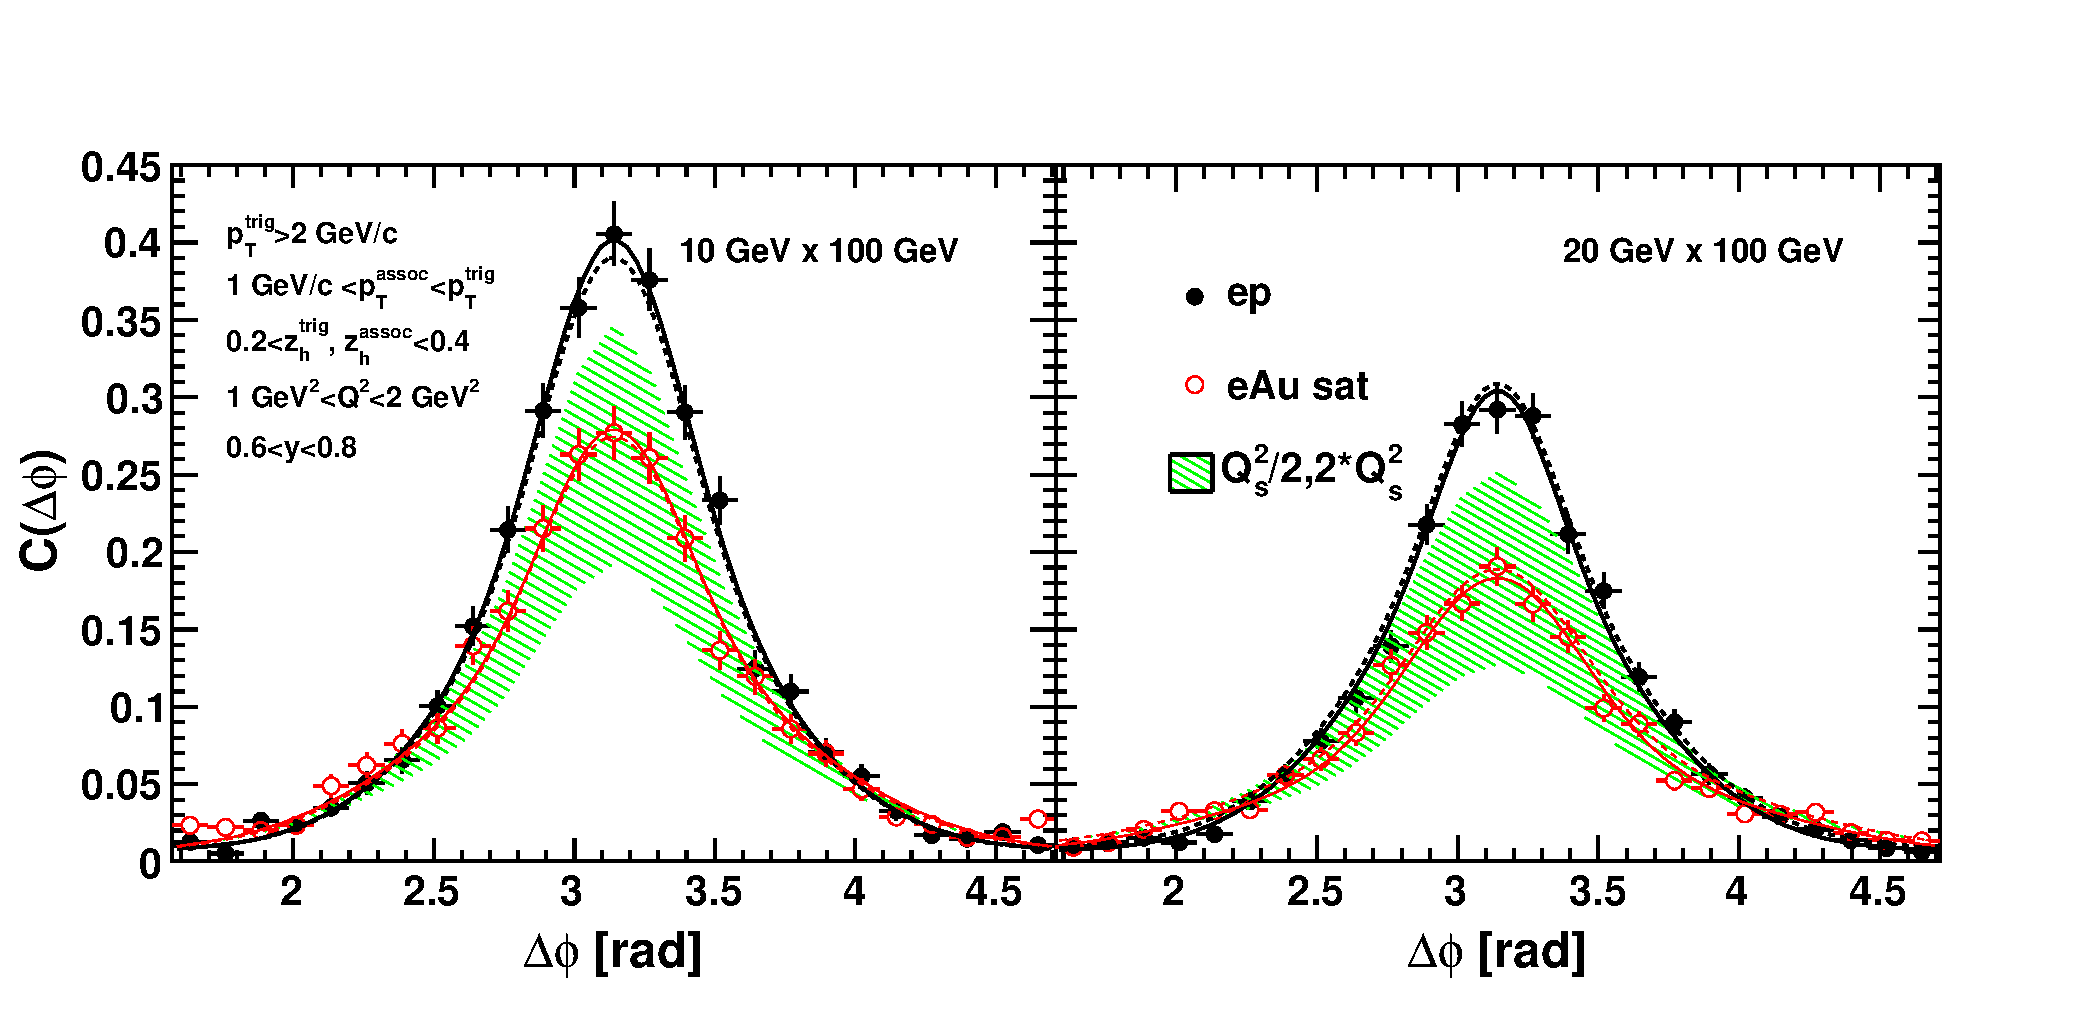
\includegraphics[width=1.0\textwidth]{plots/chpt6/Q2_1_y_0.7_varying_Qs_uncertainty_Sud_withfit_smear.eps} 
\end{center} 
\caption[correlation function with saturation scale uncertainty]{The correlation
function at $1\, \textrm{GeV}^{2}<Q^{2}<2 \, \textrm{GeV}^{2}$, $0.6<y<0.8$ for an  
integrated luminosity of $1 \, fb^{-1}$. The \ep\ result comes from PYTHIA simulations.
The $e+$Au results are a combination of simulations from a saturation-based model plus modified
PYTHIA simulations. The suppression factor uncertainty was estimated by varying
$Q_{s}^{2}$ by a factor of 0.5 and 2. Sudakov resummation has also been incorporated
for \eAu. The solid lines represent a fit for the simulated pseudo-data
including detector effects; the dashed line excludes detector effects.}
\label{fig:correUncertainSud}
\end{figure*}

In Fig.~\ref{fig:correUncertainSud} we compare the strength of the
coincidence probability based on a theoretical saturation model prediction for
the away-side for \ep\ and $e+$Au. The filled circles in
Fig.~\ref{fig:correUncertainSud} are simulated with PYTHIA
for \ep\ collisions, including detector smearing and acceptance effects.
The projected $e+$Au saturated correlation function (open circles) is
obtained by multiplying the \ep\ histogram with the suppression factor
$w^{s}_{i}=C(\Delta\phi)_{eAu}/C(\Delta\phi)_{ep}$ including Sudakov effects extracted
from Fig.~\ref{fig:dihadron_theory_sud}. This suppression factor can only be applied to
dijet channels involving gluons; namely PGF and resolved $qg\rightarrow qg$,
$gg\rightarrow gg$, $gg\rightarrow q\bar q$ subprocesses. The other quark
initiated subprocesses have been simulated with PYTHIA using the non-saturated
\eA\ model including nuclear PDFs and final-state energy loss. The uncertainties
represent the statistical precision from an integrated luminosity of 1
fb$^{-1}$. The solid (dashed) lines in Fig.~\ref{fig:correUncertainSud} represent
fits to the simulated data points with (without) detector effects included in
the simulation.

Since to date there is no exact knowledge of the saturation scale, the
uncertainty in the suppression factor is estimated by varying the saturation
scale by a factor of 0.5 and 2. The resulting uncertainty bands are depicted in
Fig.~\ref{fig:correUncertainSud}. The suppression of the away-side peak remains
significant even with this additional uncertainty compared to the $e+$Au curve
shown in Fig.~\ref{fig:dihadron_base} accounting for nuclear effects in the
parton distribution functions, energy loss effects and the resonance decay. In
summary, the suppression effects on dihadron correlations due to saturation can
be clearly discriminated from effects based on classical nuclear medium
modifications with a well-designed EIC machine.


\section{Summary}\label{sec:dihadronsummary}

Through detailed analysis, we have shown the capability of a proposed EIC
to perform dihadron correlation measurements. It
is proven that the acceptance of the dedicated detector is wide enough to
collect all the trigger particles as well as the associated particles used in our
studies. Moreover, the onset of the projected saturation region is well covered by
the eRHIC energy regime. It will clearly be possible to do a high
precision measurement of the correlation function for dihadron production with
different nuclear beams at the proposed EIC.

In this study we also describe how this dihadron correlation function is
calculated in a saturation/CGC formalism, and provide predictions for this
measurement with or without saturation effects taken into consideration. It is
straightforward to see that a strong suppression of the away-side peak of the
correlation function is expected from saturation effects, and detector effects are
negligible on this observable. Suppression effects due to leading-twist
shadowing are significantly smaller. Therefore, the observation of such
a suppression in the dihadron correlation function measured at an EIC will be a
strong experimental evidence for the existence of gluon saturation.

Dihadron measurements at an EIC are also vital and intriguing in
that they will directly measure for the first time the behavior of the Weizs\"{a}cker-Williams
gluon distribution, about which we still know very little, and which we
can hardly extract from other measurements. The knowledge of how parton showers
behave in a nuclear medium is indispensable in obtaining a valid conclusion for the
above discussions. With the Sudakov resummation performed in the saturation
formalism, this nuclear modification of parton showers in DIS dijet process is
found to be very small at leading order. Nevertheless, there might be some
nuclear dependence in the Sudakov factor at higher orders or in the
non-perturbative part~\cite{Kang:2012am}. An EIC will also permit unique measurements
that will give a definite answer to this question. With the wide kinematic
reach and different nuclear beams, an EIC is capable of measuring the $A$
dependence of parton showers. This would require quantitative measurements of
the modification of the near-side peak of the correlation functions in a 
nucleus environment and in kinematic regions where parton showers dominate.

In conclusion, the proposed high-luminosity, high-energy Electron-Ion Collider,
together with the designed detector, can provide an ideal apparatus to study
gluon saturation with high precision through the measurement of 
the dihadron correlation function.




\chapter{Determination of collision geometry in eA} \label{chp:geometry}

Suggested in Sec.~\ref{sec:eic_eA_physics}, a wide range of nuclear effects can be
investigated with the EIC facility. For instance, the parton distributions,
especially for gluons at small momentum fraction $x$, are assumed to be largely modified by
the nuclear environment and are still unconstrained. Due to the overlap
of the gluon cloud from different nucleons, the gluon saturation effects may arise
and are thought to be amplified with a nuclear target. At an EIC, with the precise control
of $Q^{2}$ and $x$ possible by measuring the scattered electrons, this nuclear enhanced
saturation effect can be systematically pinned down with measurements such as the
longitudinal strucutre function $F_{L}$~\cite{Albacete:2009fh} and dihadron
correlations~\cite{Dominguez:2011wm}. Other than gluon saturation in the initial
state, the nuclear medium will introduce a modification to the final-state color
neutralization and hadronization. The multiplicity ratio measurement $R^{h}_{A}$
can be used to examine the time development of hadronization~\cite{Accardi:2007in}.
 
All these effects are expected to have a strong dependence on the underlying
collision geometries with respect to the nuclear environment. Gluon saturation
is closely related to the impact parameter through the thickness of nuclear
medium. Changes to the hadronization also correlate with the path length of
fast-moving color charges in the cold nuclear medium. However, there has been
little discussion about the characterization of collision geometry in individual
nuclear deep inelastic scattering (DIS) collisions up to now.

In order to characterize the geometry of collisions in proton-nucleus or nucleus-nucleus collisions, quantities
like the number of binary collisions $N_{coll}$, the number of nucleons participating in
binary interactions $N_{part}$ and impact parameter have been extensively
studied with produced particle multiplicities near central rapidity~\cite{Broniowski:2001ei}. This method has been widely used in
the determination of geometries for numerous measurements at the Relativistic Heavy Ion Collider (RHIC) and
the Large Hadron Collider (LHC)~\cite{Aamodt:2010cz,Abelev:2008ab,Back:2002uc}. Unfortunately, in
nuclear DIS studies at the moment, geometric dependence
can only be studied with the variation of nuclear target atomic number $A$,
after averaging over the geometric effect for that given nuclear type.  
%since
%the dependence on the produced particle multiplicity is too weak for \eA
%collisions due to small electron-nucleon cross section compared to
%nucleon-nucleon cross section.


In this work, we detail a description of the determination of collision geometry
for \eA\ using the neutrons emitted at forward rapidities during the evaporation
process of the target remnant. A similar technique has been used for correcting
auto-bias correlations in centrality determination of \dA\ and $p+$Pb collisions
at RHIC and the LHC~\cite{Adare:2013nff,Toia:2014wia}. We expound the design of
an \eA\ collision geometry measurement based on simulations from the DPMJET
Monte Carlo (MC) generator~\cite{Roesler:2000he}. Possible applications of this
measurement have been explored. This type of geometry control, if applied to the
observables in an \eA\ program, not only provides an additional handle on
nuclear effects but also simplifies the procedure of estimating systematic
errors. Compared to the method of scanning multiple nuclear types, one only has
to deal with the same systematic uncertainties in one nuclear type instead of
worrying about several systematic uncertainties from different nuclear beams.


The remainder of this chapter is organized as follows: in the Sec.~\ref{sec:geoDef}, we introduce the relevant
quantities utilized to describe the collision geometry and illustrate our
strategy for categorizing different geometries. The results of this categorization
are provided in Sec.~\ref{sec:geoCategory}. Possible applications of this
measurement are developed in Sec.~\ref{sec:application}. In the end, we
summarize our methods in Sec.~\ref{sec:summary}.




\section{Characterization method of collision geometry} \label{sec:geoDef}

It has been argued that the soft neutron production in lepton-nucleus collisions is
a sensitive probe of final-state interactions in the nuclear
environment~\cite{Strikman:1998cc,White:2010tu}. To our current understanding, such neutrons
are produced in the thermal emission stage of the residual nucleus left after
interactions between the fast probe and target. In the first approximation, the
soft neutron production is proportional to the number of nucleons removed in the
DIS interaction and the subsequent secondary interactions between the
particles generated in DIS process and the rest of the nucleons. In the
following discussions, it is preferable to use the target rest frame with the virtual
photon defining the longitudinal direction.

Conventionally, the procedure of an electron scattering from nucleus can be
described by the following steps. With the electromagnetic exchange, the
incoming electron emits a photon, which couples with the nucleus target.
Depending on kinematics, the photon projectile then goes through one or multiple
collisions with partons from the nucleons sitting in the photon's path, which
can be interpreted in various frameworks~\cite{Piller:1995kh}. Here, we define
the length of the projected straight trajectory of the incoming virtual photon
through the nucleus starting from the involved nucleon during the DIS process
by the traveling length $d$ in the nuclear rest frame, see
Fig.~\ref{fig:geometry}. If there are multiple nucleons involved in the DIS
scattering, $d$ is defined with an interaction point from the average position
of all involved nucleons. Therefore, in each event, one has the position of the
involved nucleon (or average position of multiple nucleons) as the
photon-nucleon primary collision vertex, as presented in
Fig.~\ref{fig:geometry}, at a displacement of $R$ from the center of the nucleus
with an impact parameter $b$.

For large nuclei, a Woods-Saxon distribution is often used to describe the 
initial nuclear density~\cite{Miller:2007ri}:
\begin{equation}
\rho(R)=\frac{\rho_{0}}{1+e^{\frac{R-R_{0}}{a}}},
\label{eqn:woodsaxon}
\end{equation}
in which $R_{0}$ corresponds to the typical nuclear radius, $\rho_{0}$ is the nucleon density in the center of the nucleus and $a$ gives the skin depth.

\begin{figure}
\begin{center}
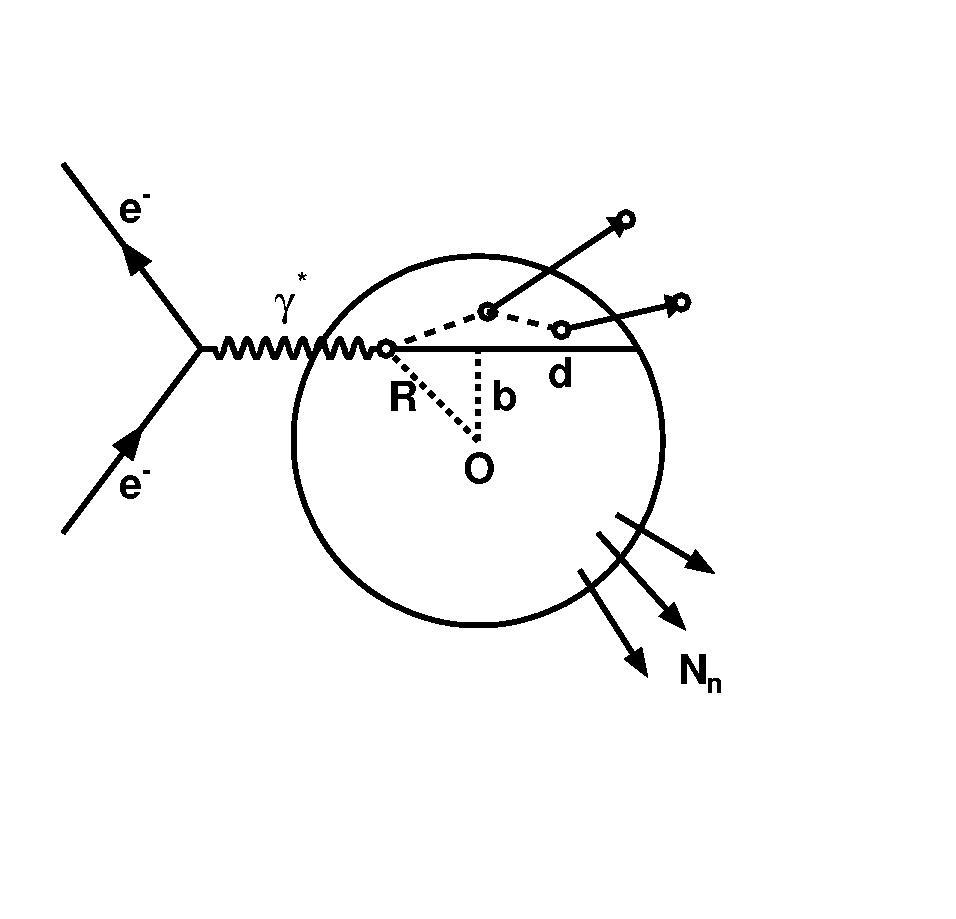
\includegraphics[width=0.5\columnwidth]{plots/chpt7/geometry_definition.eps}
\caption[A schematic view of the \eA\ collision and the relevant geometric quantity definition] {Relevant quantities to describe the collision geometry. $b$ represents the impact parameter. $R$ shows the spatial displacement of the interaction point to the center of the nucleus. $d$ is the traveling length, which defines the projected virtual photon traveling length from the interaction point to the edge of the nuclear medium.}
\label{fig:geometry}
\end{center}
\end{figure}

The hadronic fragments generated from photon-nucleon collisions may cause
sequential secondary interactions that knock out additional nucleons
not involved in the DIS interactions. This process is usually named as the
``intranuclear cascade" process~\cite{Bertini:1963zzc}.

After all the formed final-state particles leave the nucleus remnant, due to
momentum conservation, a recoil momentum will lead the residual nucleus to an
equilibrium state characterized by its mass, charge and excitation energy. At
the end of the reaction chain, the excited nucleus will break up into stable
final products, with the emission probability described by the nuclear
evaporation model~\cite{Weisskopf:1937zz}.

In the statistical evaporation model, the number of neutron emissions strongly
depends on the excitation energy, which comes from the number of nucleons removed from
the nuclear remnant, is dictated by the successive primary and secondary
interactions in the cascade process~\cite{Ferrari:1995cq}. One may find the
connection between the collision geometry and the evaporated neutron number
distribution through the traveling length $d$ defined above. The larger $d$
is, the more nucleons are expected to be involved in the sequential collisions
and removed from the nuclear remnant, and the more neutrons can be emitted during
the evaporation.


Given such a connection, one may propose that if the emitted
neutron numbers can be measured, we would have a handle to effectively
constrain the underlying collision geometries, which is missing for a long time
in the nuclear DIS studies where the averaged geometry over the whole nucleus
has typically been used. The number of neutrons emitted in the nuclear
break up process will be labeled as $N_{n}$, illustrated in
Fig.~\ref{fig:geometry}.

Once one can select for traveling length, impact parameter (centrality)
can be effectively constrained according to the traveling length. As is shown
in Fig.~\ref{fig:distBimp}, events with very central collision ($b\approx 0$)
can be acquired with the selection of the largest traveling length (covered by blue
crossings), although we may have little control on the peripheral collision
events; the region covered by red vertical lines corresponds to small traveling length, but it
is mixed with central and peripheral collisions.
\begin{figure}[hbt]
\begin{center}
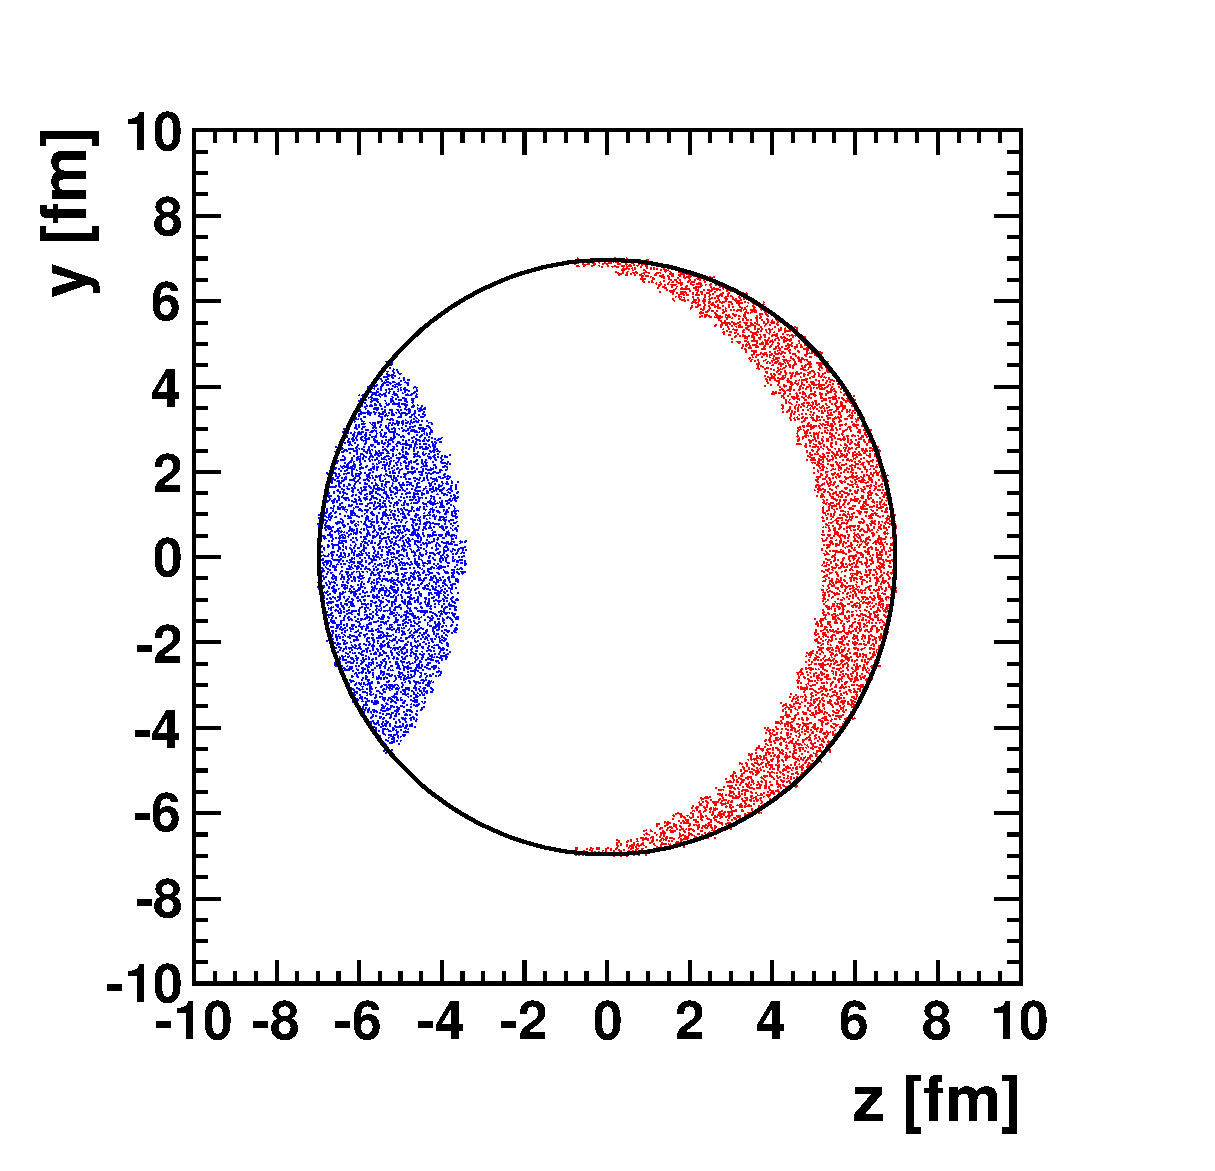
\includegraphics[width=0.55\columnwidth]{plots/chpt7/distance_to_bimpact_contour.eps}
\caption[Contour of the collision geometry selected by the specific traveling distances] 
{Schematic view showing region selected by different traveling length in $y-z$
plane with positive $z$ being the virtual photon direction in the nuclear rest
frame and $y$ being the impact parameter direction. The radius of the nucleus
has been set to $R_{0}=$6.52 fm for gold nucleus. Regions selected by
$d<0.25R_{0}$ and $d>1.5R_{0}$ are marked by red vertical lines and blue crossings, respectively.}
\label{fig:distBimp}
\end{center}
\end{figure}


The Monte Carlo generator DPMJET has been utilized in our studies to simulate
\eA\ collisions. In the Monte Carlo procedure,
initial nuclear geometric configurations are built with nucleons drawn randomly
with a radius $R$ to the center of target ion from the distribution $4\pi
R^{2}\rho(R)$ where $\rho(R)$ follows the Woods-Saxon distribution. For the
simulation of a gold nucleus, we have $R_{0}=1.12A^{1/3}=6.52$ fm and skin
depth $a=0.545$ fm~\cite{Engel:1996yb}.



The final states in DPMJET are simulated by three stages in a chain. Firstly,
the primary DIS interactions are simulated by PHOJET~\cite{Engel:1995yda}. Only
primary DIS interactions can generate particles with a hard momentum transfer.
Then, particles produced at the primary interaction become the source to trigger the
intranuclear cascade process. A formation zone concept has been introduced to
this cascade process. In the target rest frame of the DIS interaction, a
formation time $\tau$ is needed before newly created particles can re-interact
with the spectator nucleons~\cite{Ferrari:1995cq}:
\begin{equation}
\tau = \tau_{0}\frac{E}{m}\frac{m^{2}}{m^{2}+p^{2}_{\perp}},
\end{equation}
with $\tau_{0}$ being a free formation length parameter. $E$, $m$ and
$p_{\perp}$ are the energy, mass and transverse momentum for the created
particles, respectively. For each hadron, a formation time is sampled from an
exponential distribution with an average value as given above. The lower the
hadron energy is, the higher is the probability for that hadron to form inside
the nucleus. The kinematics of the secondary interactions occurring in the
cascade are treated by HADRIN~\cite{Hanssgen:1986az}. Since the nuclear remnant
undergoes equilibration before breakup, evaporative particles should follow a
thermal distribution. Details of the evaporation process are handled by
FLUKA~\cite{Ferrari:2005zk} with the input of remnant charge, mass and
excitation energy and no memory from the prior stages.

It should be noticed that this formation zone intranuclear cascade model is only
one way to describe the effect of final-state interactions in the nuclear
environment. Many other models have more sophisticated considerations with the
pre-hadron stage or parton energy loss incorporated. Phenomenological studies
have been done by adjusting the pre-hadron formation time and the final physical
hadron formation time to obtain the best description to the experimental
data~\cite{Akopov:2004ap}. Other QCD-inspired models, which are focused on the
struck quark energy loss, calculate the modifications to the fragmentation
function through gluon bremsstrahlung in a nuclear
medium~\cite{Salgado:2003gb,Chang:2014fba}. No hadron re-interaction is included
in this type of model, as the produced hadron is assumed to always form outside
the nucleus. In this work, we are mainly interested in the correlation between
the underlying geometry and the neutron emission during evaporation. Although
they are bridged through this final state interaction in the nucleus, the exact
details are not very important to our study. However, more well-developed
models, with better descriptions to the final state interaction, can be added to
our discussions in the future.


Multiple scatterings have been implemented via the Gribov-Glauber
realization~\cite{Shmakov:1988sc} in this MC model. The primary interaction is
sampled from a sequence of independent binary photon-nucleon collisions based on
an elementary photon-nucleon cross section. When we have more than one nucleon
coupled to the DIS interaction stage, the primary interaction point will be
defined as the average position of all the involved nucleons. However,
considering the elementary cross section is very small, the number of binary
collisions happened in one event is most likely to be one. Coherent scattering
effects have been incorporated as a shadowing of the elementary cross section,
based on the coherent length of the photon probe hadronic
fluctuation~\cite{Piller:1999wx}.


\section{Collision geometry categorization} \label{sec:geoCategory}

\subsection{Geometry constraint with forward neutrons}
In the following discussions, we will use an event sample
generated from DPMJET for $e+$Au at 10 GeV $\times$ 100 GeV with $1 \, \mathrm{GeV}^{2}
< Q^{2} < 20 \, \mathrm{GeV}^{2}$, $ 0.01<y<0.95$.

The evaporated products emitted during nuclear break up are most likely to be protons
and neutrons. Due to existence of the Coulomb barrier for charged fragments,
proton emission will be largely suppressed. As seen in
Fig.~\ref{fig:evapNeutronVsProton}, the number of emitted protons during nuclear
evaporation is much lower than that of neutrons from the same event.
Therefore, by measuring neutrons alone, we can characterize the major
properties of the nuclear break up process.

\begin{figure}
\begin{center}
\includegraphics[width=0.7\columnwidth,keepaspectratio]{plots/chpt7/evap_protonVsneutron.eps}
\caption[Correlation between the number of protons ($N^{evap}_{p}$) and neutrons ($N^{evap}_{n}$) during evaporation processes]{Correlation between the number of evaporated protons ($N^{evap}_{p}$) and neutrons ($N^{evap}_{n}$). Due
to the Coulomb barrier for protons, the proton emission during
evaporation process is greatly suppressed compared to that of neutron.}
\label{fig:evapNeutronVsProton}
\end{center}
\end{figure}

The zero degree calorimeter (ZDC) designed to measure neutral energy deposits
within a small radiation cone about the beam direction can be employed in the
measurement of spectator neutrons emitted with a small angle from the beam
remnant. Meanwhile, charged fragments and the noninteracted
beam remnants will be bent to larger angles out of the ZDC acceptance by
deflecting magnets. Thus, a ZDC reads out the total
neutral energy in the forward rapidities, or effectively the number of
emitted neutrons, from nuclear break up in a very clean way.

\begin{figure}
\begin{center}
\includegraphics[width=0.7\columnwidth,keepaspectratio]{plots/chpt7/tau_comparison.eps}
\caption[Average neutron number from evaporation processes versus $\nu$ compared to the E665 measurement]{Results of different formation length parameters as a function of $\nu$ in the simulation compared with the E665 data~\cite{Adams:1995nu}. $\nu$ is defined in Sec.~\ref{sec:basicDIS}. The green solid line shows the prospective $e+$Au data kinematics coverage at 10$\times$100 GeV at an EIC.}
\label{fig:tauCompare}
\end{center}
\end{figure}

There is currently only limited knowledge about the magnitude of this neutron emission
for DIS events, the only available measurement being
from E665 experiment~\cite{Adams:1995nu} at FermiLab. From the comparison of
Fig.~\ref{fig:tauCompare}, one can draw an effective formation length $\tau_{0}=9$ fm$/c$
to consistently describe the magnitude of neutron emission. At the planned EIC
energy scale, this measurement can be developed with much better precision and
even wider kinematic range, to achieve a deeper understanding of this
nuclear remnant response.


If well measured, the neutron number can be used as a handle of the collision
geometry. However, since it is impossible to directly measure the number of
neutrons, we will use the energy deposition in a ZDC to extract the neutron
number information. In the following discussions, an energy resolution $\sigma/E
= (85/\sqrt{E} + 9.1)\%$ with $E$ in GeV from Ref.~\cite{Adler:2000bd} has been used as the ZDC
responses for neutron energy. 
%The resolution of the traveling length is
%dominated by its intrinsic correlation with the number of emitted neutrons during
%the evaporation process. The assumed ZDC energy resolution, which is used in the
%current RHIC heavy ion experiments, is sufficient for our study.

\begin{figure*}[hbt!]
\begin{center} 
\subfigure[]{ 
\centering
\includegraphics[width=0.46\columnwidth,keepaspectratio]{plots/chpt7/tau9_neutron_travel_distance_corre.eps} \label{fig:distCorre} 
}
\quad
\subfigure[]{ 
\centering
\includegraphics[width=0.46\columnwidth,keepaspectratio]{plots/chpt7/tau9_neutron_bimpact_corre.eps} \label{fig:bimpCorre} 
}
\caption[Geometric quantity correlation with neutron energy deposit]
{(a) Traveling length $d$ and energy deposition in the ZDC are correlated; (b) impact parameter $b$ not as well constrained. The black solid line indicates the central value of $d$ or $b$ in the corresponding $E_{n}^{ZDC}$ bin respectively. } \label{fig:geoCorrelation}
\end{center} 
\end{figure*}



\begin{figure} 
\begin{center} 
\includegraphics[width=0.7\textwidth]{plots/chpt7/tau9_travel_dist_constrain.eps}
\caption[Geometric quantity constrained by forward neutron energy deposit binning method]
{Traveling length distribution in different forward neutron energy bins. The black solid line corresponds to peripheral collisions (66-100\%), while
the red dashed and green dotted lines correspond to the 33-66\% and 0-33\%, respectively.}
\label{fig:geoConstrain}
\end{center} 
\end{figure}


\begin{figure}
\begin{center}
\includegraphics[width=0.7\columnwidth,keepaspectratio]{plots/chpt7/tau9_neutron_bin_selection.eps}
\caption[Neutron binning method with the neutral energy deposition in ZDC]{Selections of different collision geometry with neutron number translated to energy deposition. Different colors represent different centrality selections}
\label{fig:neutronBin}
\end{center}
\end{figure}


\begin{table*}[width=0.85\columnwidth]
\centering
\begin{tabular}{ |l || l | l | l | } \hline 
		& $\Sigma E_{n}$ range [GeV] & $<d>$ / $d_{\mathrm{RMS}}$ [fm] & $<b>$ / $b_{\mathrm{RMS}}$ [fm] 	\\ \hline
0-33\%	& 743-4329		&	9.7 / 2.7	& 3.8 / 1.6	 \\ \hline
33-66\%	& 237-743		&	7.5 / 2.8	& 4.4 / 1.7	\\ \hline
66-100\%& 0-237			&	5.9 / 2.8	& 4.7 / 1.8	\\ \hline
\end{tabular}
\caption[Constrained geometric quantity with the neutron binning method]{Geometry constrained by the neutron energy deposition tagged bins. Average value as well as the root mean square (RMS) for traveling length $d$ and impact parameter $b$ has been presented in this table.}
\label{tab:geoConstr}
\end{table*}


Indicated by Fig.~\ref{fig:geoCorrelation}, energy deposition in the ZDC can be used
as a good measure of traveling length $d$ while the impact parameter $b$ is not as
well controlled. 
Only the most central events ($b\sim0$) can be selected with the largest
evaporated neutron emissions. With this correlation shown in
Fig.~\ref{fig:distCorre}, one can select a binning method to constrain the
underlying geometries. Fig.~\ref{fig:geoConstrain} shows to what extent the
traveling length $d$ can be constrained with the binning method shown in
Fig.~\ref{fig:neutronBin}. The percentage is defined by the fraction of events with
a certain energy deposition in the ZDC.
Constraints put on the quantities with statistical uncertainties under the
current binning strategy can be found in Tab.~\ref{tab:geoConstr}.


The assumed polar angular acceptance of the ZDC is $\pm$ 4 mrad with respect to
the gold nuclear beam direction~\cite{Accardi:2012qut}.
Fig.~\ref{fig:neutronZDC} shows that emitted neutrons from the evaporation
process can be $100\%$ accepted. The final state neutrons from all processes are
marked by the black solid line in that plot. The green (dash-dot) line shows neutrons from
primary interactions. Neutrons generated by intranuclear cascade are shown in
blue (dotted) and evaporated neutrons are shown in red (dashed). It can be concluded from this
plot that neutrons from primary interactions are mainly in the midrapidity
region, while the forward region neutrons are dominated by the evaporated
neutrons. The primary interaction and intranuclear cascade process can also
become a source for final state neutrons accepted by the ZDC. In the simulated
event sample, around $15\%$ of the accepted neutrons in the ZDC come from processes
like primary and secondary interactions. As to the expected detector design, all
the evaporated neutrons can be fully accepted by the experimental device and
contamination from other process is under control.

\begin{figure}
\begin{center}
\includegraphics[width=1.0\columnwidth]{plots/chpt7/neutron_ZDC_cuts.eps}
\caption[$\eta$ distribution for all final-state neutrons in an \eA\ collision]{$\eta$ distributions of final-state neutrons from various processes. Most of the evaporated neutrons can be accepted
if the ZDC covers the polar angle range of $\pm$ 4 mrad marked by the
dashed vertical line. Black (solid) lines represent all the final state
neutrons, while the red (dash), blue (dot) and green (dash-dot) lines illustrate neutron distributions
from evaporated, intranuclear cascade and primary productions.}
\label{fig:neutronZDC}
\end{center}
\end{figure}



\subsection{Possible constraint on the most central collisions with a double cut method}

The features of particle yield at different stages of the nuclear response
are particle-type-dependent. As for the neutrons, they are mostly generated
in the evaporation process from the ``cooling" of a large excited nucleus.
As shown in Fig.~\ref{fig:neutronStage}, the ZDC accepted
neutrons are mostly evaporated neutrons. By measuring the most forward
neutral energy deposition in the ZDC we can extract the statistical emission
for that event in a very clean way.

With the intranuclear cascade process, additional particles like pions
will be generated in the reaction chain between the fast moving particles
and the rest of the nucleons.
As the $p_{T}$ kick from this type of reaction is very small, charged pions
generated in this process will move to the more forward direction compared
to those pions from primary interactions.


\begin{figure}
\begin{center}
\includegraphics[width=0.7\columnwidth]{plots/chpt7/accept_neutron_from_stages.eps}
\caption[Accepted neutron number distribution from different \eA\ collision stage]{Number of neutron distributions
from different interaction stages. The black solid line shows the total number of neutrons
within the ZDC acceptance; neutrons from the thermal evaporation process are depicted
by the red dashed line, while the blue dotted line gives the distribution from secondary
interactions and particles generated in primary interactions are marked in green (dash-dotted).}
\label{fig:neutronStage}
\end{center}
\end{figure}
With the knowledge of the underlying traveling length for the collision geometry,
it is possible to define the most central collision by selecting events with the
largest neutron production, in which the incoming photon probes the densest area
of the target. The forward proton track number from break up and the charged
particle (mostly pions) yield in forward rapidities are also sensitive to the
collision geometries, as shown in Fig.~\ref{fig:bimp_corre_p_forCh}. 


\begin{figure*} 
\begin{center} 
\includegraphics[width=0.495\textwidth]{plots/chpt7/tau9_bimpact_vs_accept_proton.eps}
\includegraphics[width=0.495\textwidth]{plots/chpt7/tau9_bimpact_vs_accept_forward_charged.eps}
\caption[Correlation between the impact parameter in \eA\ collisions and the number of evaporated protons or forward charged particles]
{Correlation between the impact parameter in \eA\ collision and evaporated protons or forward charged particles. Central value in the corresponding $N^{ZDC}_{p}$ or $N^{forwd}_{p}$ bin is suggested by the solid black line in these plots.
}
\label{fig:bimp_corre_p_forCh}
\end{center} 
\end{figure*}

We will see how much we can gain as a constraint on
most central collisions if we put an additional cut on these quantities together
with that on the forward neutrons. It may be beneficial to add the large neutron emission cut
and the large proton or charged particle production cut at forward rapidity at
the same time to select the extremely central bins. Forward proton number is
measured with a perfect resolution in an assumed coverage the same as ZDC.
Forward charged particles are supposed to be counted by devices covering
$4<\eta<6$. The geometry constraint in the most central collisions is
shown in Fig.~\ref{fig:geoConstrain_central}. The shaded region displays the total
distribution for $d$ or $b$ without any cuts. To compare with the cuts made by
0-10\% selection, the magnitude of total distribution has been rescaled by 0.1 for the purpose of
demonstration. Comparing the solid line and shaded region in
Fig.~\ref{fig:geoConstrain_central} shows the forward neutron cut effectively finds
the events with most central collisions. No significant enhancement can be found
with the inclusion of the double cut method from forward proton or charged
particles. Such ZDC accepted neutron energy would be enough to select
the most central events.
\begin{figure*} 
\begin{center} 
\includegraphics[width=0.495\textwidth]{plots/chpt7/tau9_mostCentral_dist.eps} \label{fig:travelConstrain_central} 
\includegraphics[width=0.495\textwidth]{plots/chpt7/tau9_mostCentral_bimpact.eps} \label{fig:bimpConstrain_central} 
\caption[The selected impact parameter and traveling distance in the most central collisions selected under a double cut method]
{Binning constraint on traveling length $d$ and impact parameter $b$ for most
central collisions (0-10\%), with forward neutron cut only (solid line) and
neutron cut plus additional forward proton number cut (dashed line) or forward
charged hadron number cut (dotted line). The total distribution has been marked by
the shaded region with a magnitude scaled down by a factor 10 for illustration.
}
\label{fig:geoConstrain_central}
\end{center} 
\end{figure*}


\section{Applications of collision geometry constraint at an EIC}\label{sec:application}

As both initial-state and final-state effects in \eA\ collisions are highly dependent
on nuclear geometry, applying this nuclear geometry handle to our
measurements in \eA\ program at an EIC will allow us to learn more
about the nuclear medium effect. For instance, the selection of very
central collisions maximizes the probed gluon density in the initial state which
delivers more sensitivity to the expected saturation effect. $F_{L}$ and dihadron
correlation measurements are two of the important observables sensitive to this
geometry constraint. We would see stronger saturation effects in the most
central collisions compared to peripheral \eA\ events with the change of
gluon densities. This collision geometry also provides an additional dimension to
the study of final state effects. The time space feature of this fragmentation
process can be directly confronted with the nuclear medium geometry through
which one can explore the hadronization process in a more precise way.


\subsection{Energy loss measurement in the cold nuclear medium}
It has been argued that the multiplicity ratio measurement $R^{h}_{A}$ from
HERMES suggests that the space-time development of the hadronization process in
the nuclear medium can be studied with the semi-inclusive deep-inelastic
scattering process off nuclei~\cite{Airapetian:2003mi,Airapetian:2007vu,Airapetian:2011jp}. Depending on the
kinematics, the hadron formation may take place inside the nucleus, or
outside the nucleus. In general it is assumed that the struck quark forms its
full hadron identity with an average formation length $l_{h}\propto f(z)\nu$. $f(z)$ is a general function of $z$.

The multiplicity ratio $R^{h}_{A}$ is a frequently studied quantity
which effectively describes the nuclear medium effect. It is defined as follows:
\begin{equation}
R^{h}_{A}=\frac{(\frac{N_{h}(\nu,Q^{2},p^{2}_{T},z)}{N_{l}(\nu,Q^{2})})_{A}}{(\frac{N_{h}(\nu,Q^{2},p^{2}_{T},z)}{N_{l}(\nu,Q^{2})})_{D}},
\end{equation}
where $N_{h}$ is the semi-inclusive production of hadrons in a given kinematics
bin and $N_{l}$ is the yield of leptons in the same $\nu,Q^{2}$ bin. This ratio
is defined for the hadrons production per deep-inelastic scattering event on a
nuclear target with mass $A$ to that of the lightest isoscalar nuclear target
deuterium. $R^{h}_{A}$ is expected to be less than unity due to the parton energy loss in the nuclear medium.

With a handle to constrain the traveling length in the
collision geometry, it is possible to explore the interplay between color
object neutralization and the nuclear environment geometry. If it is possible to
control the traveling length $d$ of the struck quark, one has an additional
dimension in this measurement which changes the measurement from
\(N_{h}(\nu,Q^{2}p^{2}_{T},z)\) to \(N_{h}(\nu,Q^{2}p^{2}_{T},z,d) \).
Instead of varying the different nuclear types, the hadron formation length can be
directly adjusted with a traveling length $d$; if $d>l_{h}$ it is generally
formed inside the nucleus and the hadron yield will be suppressed while for
$d<l_{h}$ the medium modification is supposed to be small. With the bin
selection of collision geometry, we have extracted the $d$ distribution from
these bins as input to an energy loss model~\cite{Salgado:2003gb} (also see Sec.~\ref{sec:energy_loss} for more details). Thereby,
strong nuclear medium dependence is expected in the multiplicity ratio
measurement, shown in Fig.~\ref{fig:energyLoss}.

\begin{figure}
\begin{center}
\includegraphics[width=0.7\columnwidth,keepaspectratio]{plots/chpt7/energyloss_Hermes_nu_qHat_0.85_tau_9.eps}
\caption[Energy loss measurement on Xenon target with several centrality bins versus $\nu$.]{Multiplicity ratio as a function of $\nu$ with the traveling length constraint. The black line represents the expected value for minimum bias events, and projected result from three centrality bins are shown in blue, green and red according to our selection discussed in Sec.~\ref{sec:geoCategory}. HERMES data points~\cite{Airapetian:2007vu} are shown in the plot with black dots.}
\label{fig:energyLoss}
\end{center}
\end{figure}



\subsection{Dihadron correlation measurements to probe gluon saturation}

In the small $x$ limit, gluon density in the nucleon becomes so large that a
phenomena named saturation may emerge. It is suggested in this scenario that, when the probe
resolution $Q^{2}$ is less than the saturation scale $Q^{2}_{s}$, the gluon
recombination mechanism becomes dominant, which tames the rapid growth of
gluon density at small $x$. According to the collision
geometry, stronger saturation is expected for the most central collisions. If
this type of physics exists, evaporated neutron number can be used as an
additional handle, together with the kinematics control, for studying the saturation effect.

Dihadron correlations in \eA\ are a way to investigate the saturation effect. By
selecting the trigger associate particle pairs with certain $p_{T}$, one can
explore the underlying jet properties and the interplay with the saturation
scale $Q_{s}$. The correlation function is constructed as shown in Chap.~\ref{chp:dihadron}:
\begin{equation}
C(\Delta\phi)=\frac{N_{pair}(\Delta\phi)}{N_{trig}}.
\end{equation}
With a scaling model, the saturation scale can be parameterized as
$Q_{s}^{2}=A^{1/3} c(b)(\frac{x}{x_{0}})^{-\lambda}$, with $x_{0}=3.04\time
10^{-4}, \lambda = 0.288$. $c(b)$ defines the thickness of the nuclear medium at
impact parameter $b$. Significant saturation effects arise when $Q_{s}$ is
large, which means collisions with smaller $x$ or larger thickness favor a
stronger saturation effect.

Following the formalism in~\cite{Zheng:2014vka}, one can estimate the centrality
dependence in \eA\ dihadron correlations, which is coordinated by the parameter $c(b)$.
From the simulation based on our centrality definition above, we can select the
events with the most central and most peripheral collisions. Observable suppression
is expected from peripheral to central events.

Fig.~\ref{fig:dihadron_centrality} shows the predicted saturation impact on dihadron correlations with an integrated luminosity of 10 fb$^{-1}$ at the energy of $\sqrt{s}=63$ GeV.
The effect of selecting the most central collisions has been studied. The thickness function is estimated by
a Woods-Saxon density as in Eq.~\ref{eqn:woodsaxon}. For 0-10\% centrality $c(b)=0.75$, while $c(b)=0.59$
for a minimum bias (0-100\%) estimation. With the current statistical uncertainty, the most central category can be slightly distinguished from the minimum bias collisions. If the ratio of correlation function from central divided by minimum bias is less than 1, as suggested by Fig.~\ref{fig:dihadron_ratio}, it could be an indication of impact parameter dependence from saturation.


\begin{figure*}[hbt!]
\begin{center}
\subfigure[]{ 
\centering
\includegraphics[width=0.46\textwidth]{plots/chpt7/dihadron_centrality_tau_9_lumi_10fb_20x100.eps}
}
\quad
\subfigure[]{ 
\centering
\includegraphics[width=0.46\textwidth]{plots/chpt7/dihadron_ratio_centrality_tau_9_lumi_10fb_20x100.eps} \label{fig:dihadron_ratio} 
}

\caption[Dihadron correlation function with centrality bin cut.]{Saturation effects in the dihadron correlation measurements with the most central collisions. (a) The correlation functions for \ep, $e+$Au 0-100\% and $e+$Au 0-10\% at 20 GeV$\times$100 GeV are shown in black, blue and red curves with the statistical uncertainty from an integrated luminosity of 10 fb$^{-1}$; (b) the ratio of the correlation function for $e+$Au 0-10\% divided by 0-100\%.}
\label{fig:dihadron_centrality}
\end{center}
\end{figure*}





\section{Summary} \label{sec:summary}

We have presented detailed studies on the determination of collision geometry
in \eA\ collisions. Utilizing the DPMJET Monte Carlo generator, we have found a
correlation between the traveling length and the number of neutrons evaporated
from the nuclear remnant. This neutron number distribution can be measured with
a ZDC in the Au-going direction with the systematics under control. All the
devices needed for this measurement have been included in the current EIC
detector design. Therefore, it is very easy to acquire this measurement
with little additional investment. Constraining collision geometry
quantities like traveling length is very meaningful in the studies of cold
nuclear medium effects. A demonstration of using this approach to make
fine traveling length binning of performing nuclear medium energy loss studies
and explore the signature of saturation physics has been provided. With the
determination of collision geometry in these measurements, our understanding of 
nuclear structure can be constrained with higher precision.



\chapter{Summary and outlook} \label{chp:summary}

In this thesis, dihadron correlation measurement as a probe for the saturation
physics has been studied. The feasibility of performing this measurement at a
future EIC is explored with our Monte Carlo simulation method. We have also
discussed the possibility of carrying out a collision geometry study in \eA\,
which may be applied to the dihadron correlation measurement and providing
additional systematics control.

An analysis accounting for gluon radiation in the calculation of the dihadron
cross section in \eA\ through Sudakov factor within the saturation framework has
been included. Based on the knowledge of this correction one can make a
comparison with the theory calculation and the future EIC data. In order to
understand the sensitivity of this dihadron correlation measurement to gluon
saturation, a non-saturation based model has been developed in our studies based
on the widely used \ep\ Monte Carlo generator PYTHIA interfaced with the nuclear
PDF and the cold nuclear medium energy loss effect. On the other hand, a
measurement of constraining collision geometry for \eA\ has been proposed and
investigated. This measurement can be easily performed by measuring neutral
energy deposition in the ZDC, which is very vital and beneficial for the \eA\ program at an EIC. 

This thesis summarized the many studies performed in the course of investigating
the saturation physics and the interesting results thus obtained. After all, there
are still open questions and ideas for future studies based on the current
results.

It could be very interesting to further understand the nuclear dependence of the
Sudakov factor in dihadron correlations. Currently, it is found that there's no
nuclear medium dependence for this Sudakov factor (parton shower) at leading
log. More sophisticated estimations need the input of experimental data to
constrain higher order effects. The forthcoming \pA\ data may shed some light on
the determination of this nuclear modification. Along with that, we probably
need more robust model independent way to estimate the impact of the collision
geometry control over various observables. This geometry control if achieved
will definitely bring us a new way of thinking about the nuclear effect in the
future \eA\ data.



%\include{appendix}

\end{CJK*}

%\bibliographystyle{plain}
\bibliographystyle{uclathes}
\bibliography{reference}

\clearpage
%
%\addcontentsline{toc}{chapter}{Presentations and publication List}
\chapter*{Presentations and publication List}
\addcontentsline{toc}{chapter}{Presentations and publication List}
%\hspace {0.75cm}
%%%%%%%%%%%%%%%%%%%%%%%%%%%%%%%%%%%%%%%%%%%%%%%%%%%%%%%%%%%%%%%%%%%%%%%%%%%%%%%%%%%%%%%%%%
%{\Large{\bfseries{Presentations}}}

\section*{Presentations}

\begin{enumerate}
  
\item Jun. 2014, Characterizing eA collision geometry with forward neutrons at an EIC, oral presentation,
  \textbf{Electron-Ion Collider Users Meeting}, Upton, NY, USA
  
\item Oct. 2013, Studies of e+A physics at an EIC, oral presentation,
  \textbf{Fall meeting of the Division of Nuclear Physics of the American Physical Society}, Newport News, VA, USA
  
\item Nov. 2012, Monte Carlo Simulation Techniques Used in the Study of Different Physics Channels at the Future eRHIC Project, oral presentation,
  \textbf{BNL Young Researcher Symposium}, Upton, NY, USA  
  
\item Oct. 2012, Dihadron Correlations in the eA program at an Electron Ion Collider, oral presentation,
  \textbf{Fall meeting of the Division of Nuclear Physics of the American Physical Society}, Newport Beach, CA, USA

\item Jul. 2012, Dihadron Correlations at eRHIC and Monte Carlo Development, oral presentation,
  \textbf{Riken BNL Research Center Workshop on Forward Physics at RHIC}, Upton, NY, USA

\item Oct. 2011, Studying the nucleus via dihadron correlation with an Electron-Ion Collider, oral presentation,
  \textbf{Fall meeting of the Division of Nuclear Physics of the American Physical Society}, East Lansing, MI, USA

\item Aug. 2010, Equillibrium Thermostatistics for Finite System with Energy Nonextensivity, oral presentation,
  \textbf{The 16th National Conference on Condensed Matter Theory and Statistical Physics}, Changchun, Jilin, China
\end{enumerate}

%%%%%%%%%%%%%%%%%%%%%%%%%%%%%%%%%%%%%%%%%%%%%%%%%%%%%%%%%%%%%%%%%%%%%%%%%%%%%%%%%%%%%%%
%{\Large{\bfseries{Publication list}}}

\section*{Publication list}

\begin{enumerate}

\item \textbf{L. Zheng}, E.C. Aschenauer, J.H. Lee, Determination of Electron-Nucleus Collision Geometry with Forward Neutrons,
  arXiv:1407.8055
  
\item \textbf{L. Zheng}, E.C. Aschenauer, J.H. Lee, Bo-wen Xiao, Probing Gluon Saturation through Dihadron Correlations at an Electron-Ion Collider ,
  Proceedings of Science (DIS2014), 255, 2014
  
\item \textbf{L. Zheng}, E.C. Aschenauer, J.H. Lee, Bo-wen Xiao, Probing Gluon Saturation through Dihadron Correlations at an Electron-Ion Collider ,
 Phys. Rev. D, \textbf{89}, 074037, 2014
 
\item \textbf{Zheng L}, Li W, Thermoequilibrium statistics for a finite system with energy nonextensivity,
Chinese Sci. Bull., \textbf{56}, 3666, 2011

\end{enumerate}


\section*{EIC Publications}
\begin{enumerate}
\item A. Accardi et al., Electron Ion Collider: The Next QCD Frontier - Understanding the glue that binds us all,
 arXiv:1212.1701
 
\item E.C. Aschenauer et al., eRHIC Design Study: An Electron-Ion Collider at BNL, arXiv:1409.1633

\end{enumerate}



%\addcontentsline{toc}{chapter}{Acknowledges}
%\chapter*{\LARGE  \bfseries {致\ \ \ \ \ \ 谢} }
\addcontentsline{toc}{chapter}{Acknowledgment}


%首段空两格
\qquad
五年多的硕博生活即将走到终点。回望走过的日子,有太多的人在其间给予过我很多的帮助。仓促成文之际,只能在这里
对他们简短地表达一下自己的谢意。

首先要由衷地感谢我的导师蔡勖教授多年的关心和指导。他渊博的学识,高屋建瓴的学术见解和认真忘我的工作态度为我树立了
人生的标杆。他为我创造的科研条件让我在硕博阶段的学习中受益颇多。因为他一贯的支持和鼓励也使我有勇气在博士阶段
去尝试一个完全不同的领域。

感谢布鲁克海文国家实验室的Jeong-Hun Lee研究员。我在BNL的三年多时间里,非常感谢他对我生活上的关心和学术上的指导。
他清晰的物理图像和对物理问题的深刻洞察力经常会让我在和他讨论问题的时候有豁然开朗的感觉。他和学生平等相处的态度
以及对学生观点的尊重让我的科研能力得到了充分的锻炼。

感谢殷中宝教授给我介绍了参与EIC项目的机会,并一直督促我在BNL的学习工作。在我论文撰写的过程中,
殷中宝教授不厌其烦地帮我修改论文的细节还提出了很多宝贵的建设性建议,使我能够在相对有限的时间里及时完成博士论文
的撰写工作。他丰富的研究经验和严谨的治学态度给我的研究和生活都带来了很多新的启示。

感谢李炜教授对我学业上的指导。从本科阶段的毕业论文工作到研究生阶段复杂系统的研究,李炜教授的指导为我
整个研究生阶段的工作打下了坚实的基础。他身上所体现出的对科学的热爱和严谨的科研精神将使我受益终身。

感谢肖博文教授在我博士期间的工作中对我的帮助。他在我刚刚接触相关工作的时候就用深入浅出的语言帮我讲解了
整个研究工作的理论基础,并且花了很多时间去回答我不理解的技术性问题,提出了很多新颖而有创见性的意见,给
我的研究工作带了很多重要的新思路。而他勤勉的工作态度,忘我的研究精神更是我在人生道路上的学习榜样。

感谢池丽萍老师和杨纯斌老师在我们的小组讨论中对我学业上的指导。感谢周代翠老师对我学业上的帮助以及在我准备博士答辩期间为我提供的便利条件。感谢粒子所王恩科老师,刘峰老师,
杨亚东老师,侯德富老师,刘复明老师,付菁华老师,许明梅老师在平时学业上对我的教诲。感谢
高燕敏老师,谢晓梅老师,马亚老师,刘海涛老师,刘超老师,葛静老师对我们生活上的关心,为我们提供了良好的学习工作
条件。

感谢复杂系统小组的各位师兄师姐:郭龙,江健,辜姣,惠子,邓为炳,曹燕青,赵婷婷,还有王杜鹃同学和各位师弟师妹:朱月英,
骆增增,章可成,粟柱,赵龙峰,韩继辉,邹以江,褚晓璇,何长洋,张文俊,邓盛峰,刘光环,王冰冰,王可,徐高。感谢你们给了
我一个大家庭般的温暖。

感谢ALICE小组的几位师弟:张永红,詹扬,彭忻烨,任小文,罗文钊。感谢你们在我准备博士论文及答辩期间的热心帮助。

感谢在华师读研以来风雨相伴的几位同窗好友:龚晖,陈蔚,刘可,饶识,吴妍,谷文举,伊珍,李延芳,曾世碧,朱剑辉,罗覃,
张瑛,张煜,鄢君。有你们在的日子,从来就不会缺少欢乐,感谢你们陪我走过这一段难忘的岁月。

感谢柯宏伟,仇浩和杜成民在我初到BNL时对我的悉心帮助。在异国他乡的不适应中,你们教会了我做饭的生存技能,
帮助我在一片浑浑噩噩的状态中安顿下来。感谢陈丽珠,朱逾卉,崔相利,黄炳矗,赵杰,薛亮,李玄,杨岩,辛科峰,韩立欣等几位师兄师姐在学业上
和生活上给我的莫大帮助。感谢查王妹,寿齐烨,阎威华,杨驰,郭毅,胡雪野,徐亦飞,杨帅,张金龙,张正桥,王旭,杨钱,周龙,黄欣杰,冯照
等小伙伴在BNL的朝夕相伴。感谢邓建老师,邵明老师,唐泽波老师,张一飞老师,王亚平老师,裴骅老师,施梳苏老师和王晓蓉老师在BNL期间对我的照顾。

感谢刘嘉师兄和郝阳师姐在我们的英语学习小组中对我的帮助。和你们一起经历的挑战让我觉得这世上没有不能克服的困难。


感谢亲爱的父亲母亲一直以来对我的支持。我能理解很多时候你们所承受的压力比我还要大,
所以我非常感激你们愿意去支持我所做出的每一个决定。


当五年多的时光化作手中这本薄薄的毕业论文,很难想象一段超过二十分之一的人生旅程就要在这里做出一个小小的总结。
重新翻过自己的论文,好像看到的都是这五年多的点点滴滴:有在处理未知问题时的忐忑不安,有在寻求解决方案时的辗
转反侧,有在完成一个小任务时的暗自得意,也有在看到新方向时的兴奋不已。翻过这一页,是道别,也是启程。感谢那
些陪我一路走来的人们,你们让我前进的每一步都有了存在的意义。



\end{document}
